\documentclass[10pt, oneside]{book}
\usepackage[utf8]{inputenc}
\usepackage{amsmath}
\usepackage{amsthm}
\usepackage{amssymb}
\usepackage{enumitem}
\usepackage{mdframed}
\usepackage{hyperref}
\usepackage{esint}
\usepackage{multirow}
\usepackage{systeme}
%\usepackage{moresize}
\usepackage{relsize}
\usepackage{xcolor}
\usepackage{comment}
\usepackage{cancel}
\usepackage[a4paper,left=2.3cm, right=2.3cm, top=2.1cm, bottom=2.1cm]{geometry}
\usepackage[italian,greek]{babel}
\usepackage{ragged2e}
\usepackage{fancyhdr}
\usepackage[Conny]{fncychap}
%\ChTitleVar{\raggedleft\Huge\bfseries\fontfamily{cmss}\selectfont}
\usepackage{tikz}
\usepackage{pgfplots}
\usetikzlibrary{decorations.pathreplacing,calligraphy}
\usetikzlibrary { decorations.pathmorphing, decorations.shapes, }
\usepackage[cal=dutchcal]{mathalfa}
\usepackage{wrapfig}
\usepackage{physics}
\usepackage{listings}
\usepackage{graphicx}
\usepackage{eso-pic, transparent}
\usetikzlibrary{calc}
\usetikzlibrary{positioning}
\pgfplotsset{width=10cm,compat= newest}
\usepgfplotslibrary{external}
%\tikzexternalize
\usepackage{bbold}
\swapnumbers
\hypersetup{
    colorlinks=true,
    linkcolor=blue,
}
 
\renewcommand{\arraystretch}{1.3}
\setlength{\tabcolsep}{0.5cm}

\renewcommand{\qedsymbol}{\hfill \large $\blacksquare$}
%\renewcommand{\descriptionlabel}{$\ast$}
\newcommand{\evolt}{\, \mathrm{eV}}
\newcommand{\celsius}{\, \mathrm{{}^\circ C}}
\newcommand{\newton}{\, \mathrm{N}}
\newcommand{\kelvin}[1]{\, \mathrm{K^{#1}}}
\newcommand{\joule}[1]{\, \mathrm{J^{#1}}}
\newcommand{\angstrom}{\, \mathrm{\AA}}
\newcommand{\meters}[2]{\, \mathrm{#1 m^{#2}}}
\newcommand{\coulombs}[2]{\, \mathrm{#1 C^{#2}}}
\newcommand{\grams}[1]{\, \mathrm{g^{#1}}}
\newcommand{\mols}[1]{\, \mathrm{mol^{#1}}}
\newcommand{\limit}[2]{\lim\limits_{#1 \rightarrow #2}}
\newcommand{\mean}[1]{\langle #1 \rangle}
\newcommand{\infobox}[2]{\vspace{0.5cm}~\\ \textbf{#1} \hrulefill \vspace{0.2cm}\\#2 {}\,\\\hrule \vspace{0.5cm}}
\newcommand{\lawbox}[2]{\begin{center}
\framebox{
\parbox{\linewidth}{
\vspace{0.3cm}
\textbf{#1} \hfill $\displaystyle #2$
\vspace{0.3cm}
}
}
\end{center}}

\newcommand{\lawboxtext}[2]{\begin{center}
\framebox{
\parbox{\linewidth}{
\vspace{0.3cm}
\textbf{#1} \vspace{0.1cm} \\#2
\vspace{0.3cm}
}
}
\end{center}}

\newcommand{\ds}{\displaystyle}
\newcommand{\tendsto}[2]{\xrightarrow[#1 \rightarrow #2]{}}
\newcommand{\integral}[4]{\int_{#1}^{#2} #3 \, \mathrm{d}#4}
\newcommand{\setel}[1]{ \{ #1\} }
\newcommand{\setprop}[3]{ \{ #1 \, \in \, #2 \, : \, #3 \}}
\def\upint{\mathchoice%
    {\mkern13mu\overline{\vphantom{\intop}\mkern7mu}\mkern-20mu}%
    {\mkern7mu\overline{\vphantom{\intop}\mkern7mu}\mkern-14mu}%
    {\mkern7mu\overline{\vphantom{\intop}\mkern7mu}\mkern-14mu}%
    {\mkern7mu\overline{\vphantom{\intop}\mkern7mu}\mkern-14mu}%
  \int}
\def\lowint{\mkern3mu\underline{\vphantom{\intop}\mkern7mu}\mkern-10mu\int}
%\def\derx{\frac{\textrm{d}^2}{\textrm{d}x^2}}

\title{SIOLI'S LECTURES ON THERMODYNAMICS}
\author{Alberto Zaghini}
\date{a.a. 2022-2023}

\begin{document}
\selectlanguage{italian}

\makeatletter
\begin{titlepage}
\vspace{-2.1cm}
\AddToShipoutPictureBG*{%
  \AtPageLowerLeft{%
    \transparent{1}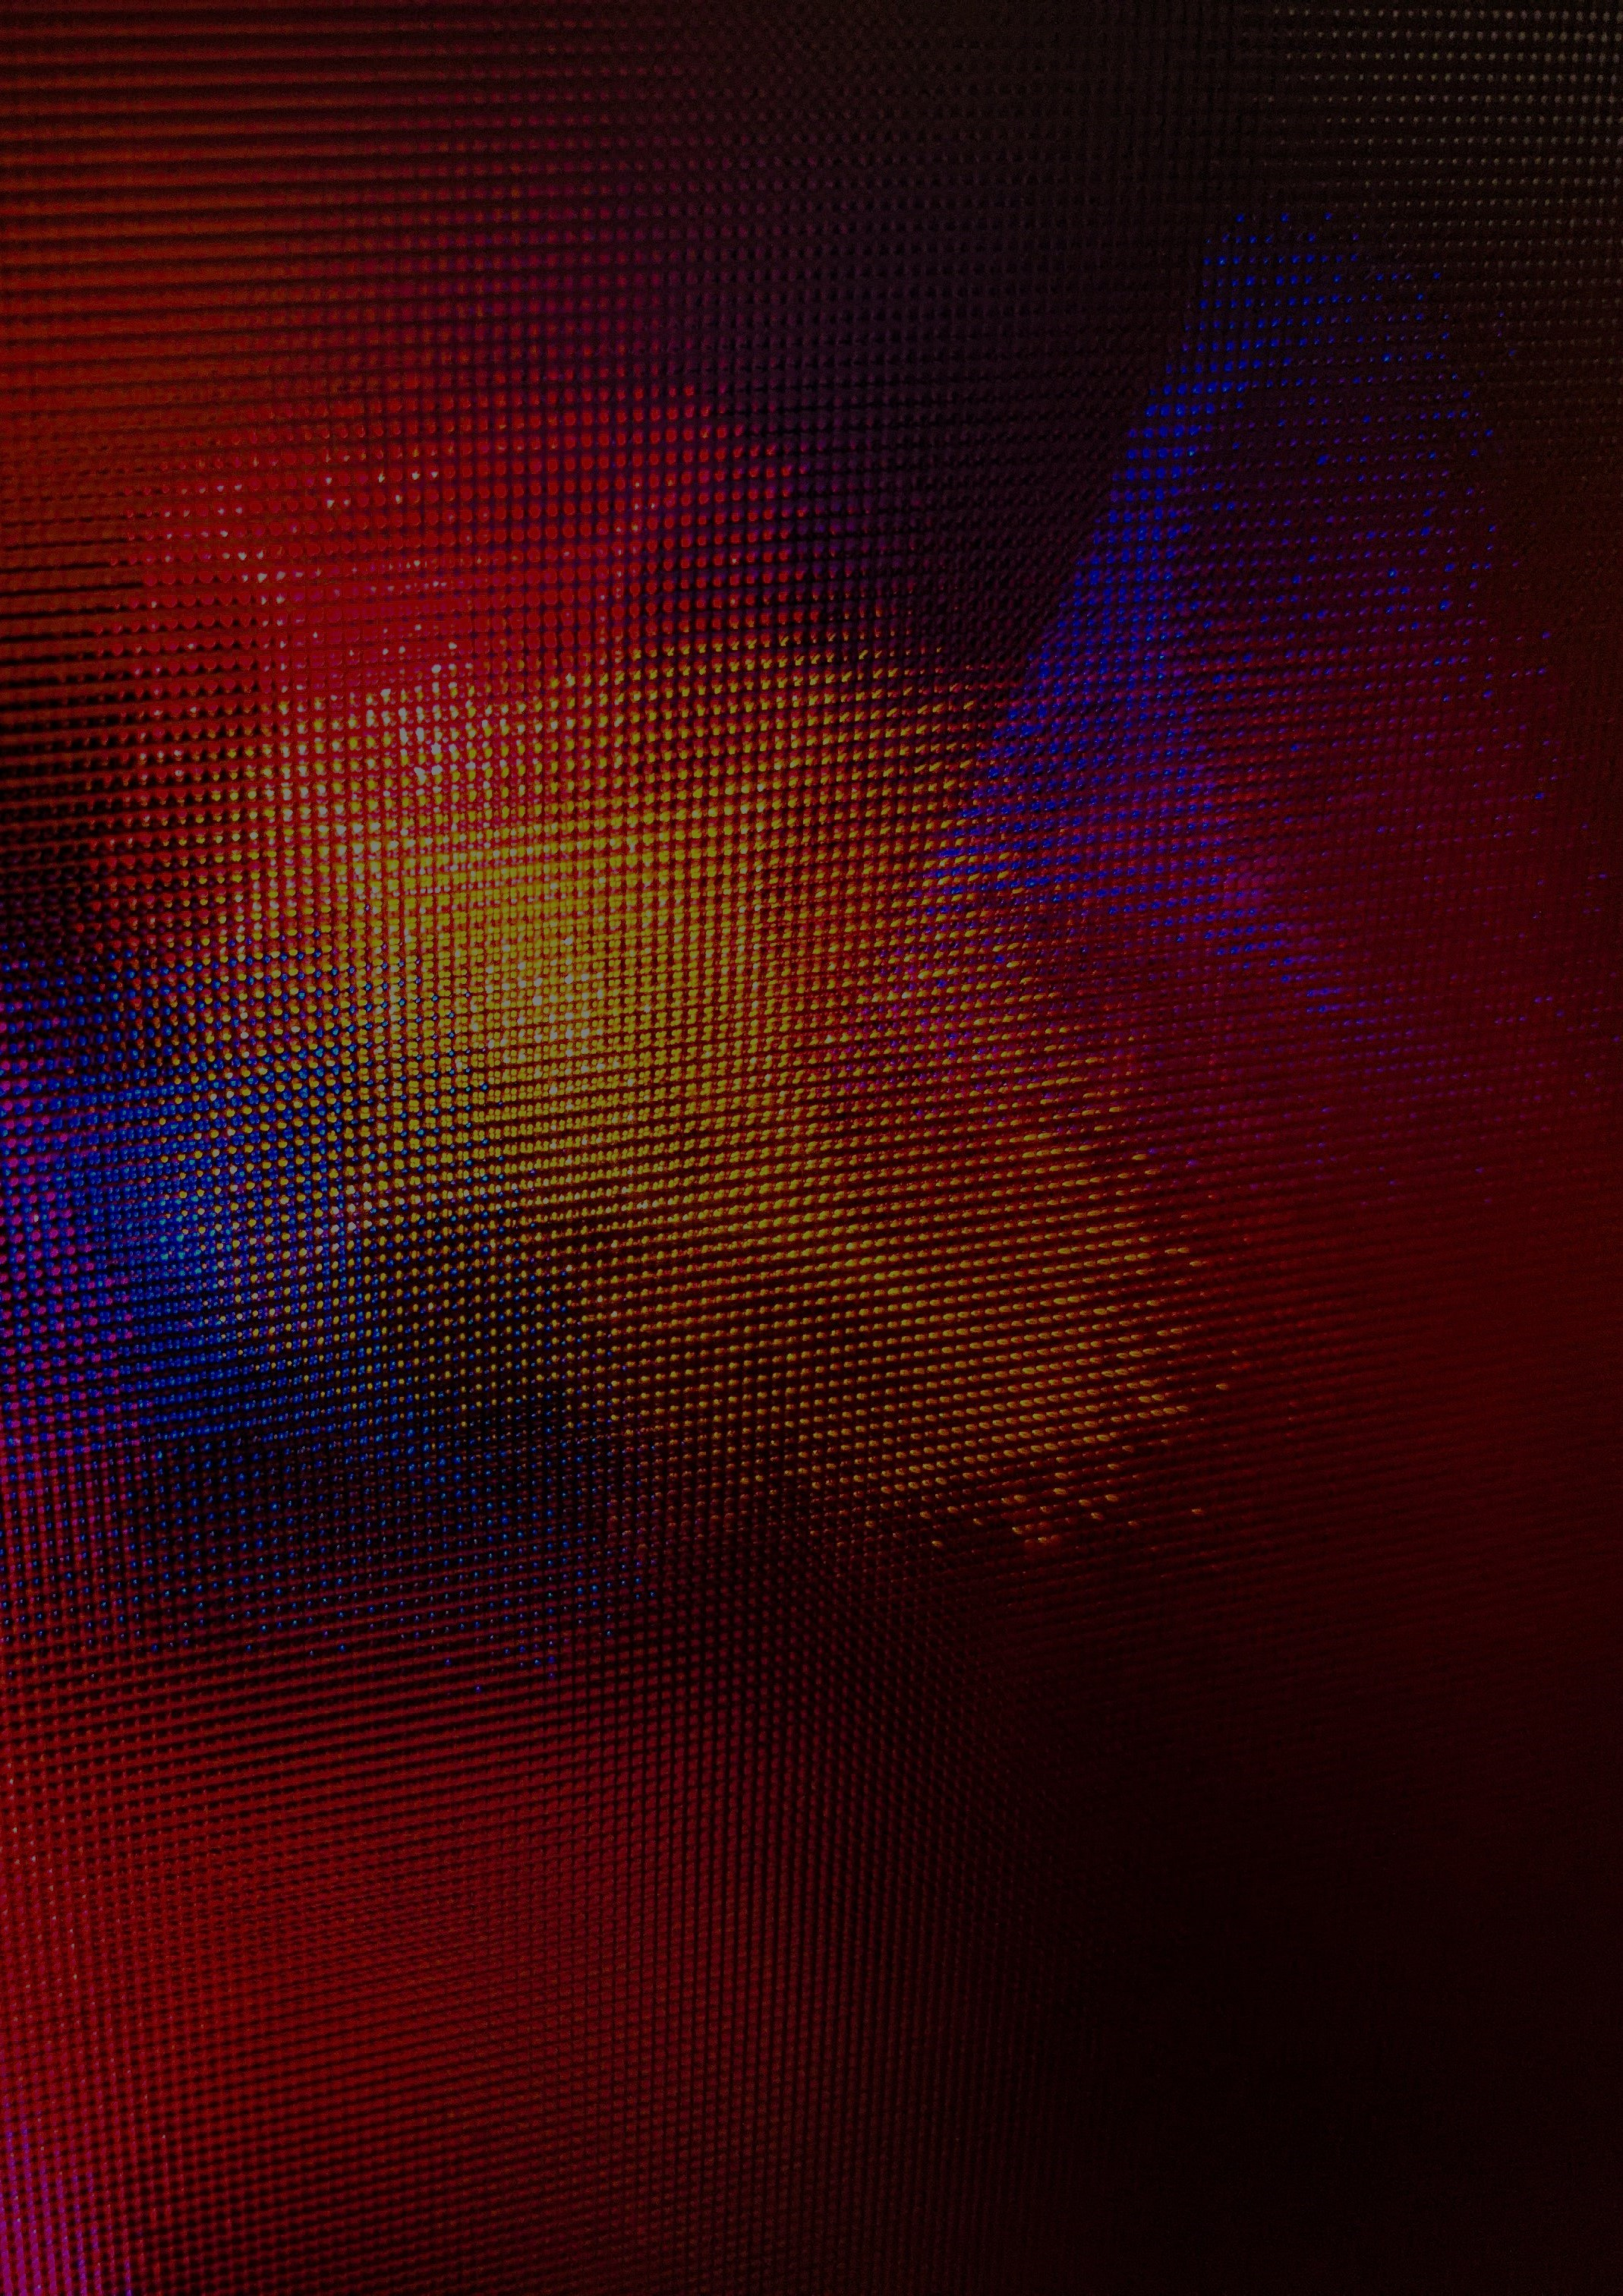
\includegraphics[width=\paperwidth,height=\paperheight]{cover.jpg}%
  }%
}
\hspace{0cm}
\vfill
\color{white}
\, \\\larger[20]\textsf{\textbf{RSZ's TREATISE ON\\ELECTRICITY AND MAGNETISM}}
\\\smaller[2]Alberto Zaghini
\\a.a. 2023-2024
\\~\\ \larger[20]\,\,
\\~\\ \,\,

\vfill
\hspace{0cm}
\end{titlepage}
\makeatother
\selectlanguage{italian}

\tableofcontents
\newpage

\setcounter{chapter}{-1}

\chapter*{Introduzione}

Il presente testo è un compendio per il corso di \textit{Elettromagnetismo} del CdL triennale in Fisica dell'Università di Bologna. I contenuti sono quelli del corso tenuto nell'a.a. 2023-2024 dai docenti Lorenzo Rinaldi, Roberto Spighi e Antonio Zoccoli - da cui la sigla nel titolo, che è peraltro una citazione dell'opera fondamentale di James Clerk Maxwell in cui fu per la prima volta esposta la teoria completa dell'elettromagnetismo classico. 
\\Pur essendo stata la nostra la prima coorte suddivisa tra i canali A-L ed M-Z, il corso è stato svolto congiuntamente per entrambi; non si ha garanzia sarà così anche per gli anni a venire. Mi auguro il testo possa essere utile anche in caso dovessero subentrare nuovi docenti per uno dei due canali.
\\Questi appunti sono stati redatti a partire in primis dai contenuti delle lezioni, integrati talvolta con i libri di Mazzoldi-Nigro-Voci, Griffiths, Feynman, Jackson, Purcell-Morin.

\begin{center}
\textit{L'edizione attuale è da considerarsi una bozza provvisoria. \'E mia intenzione aggiungere quando possibile figure e ulteriori integrazioni dai testi di riferimento.}
\end{center}
Buono studio!

\chapter{Complementi di analisi vettoriale}

\section{Gradiente}

Sia dato un \textbf{campo scalare}, ovvero una funzione

\[\varphi \, : \, \mathbb{R}^3 \rightarrow \mathbb{R} \qquad \varphi \, : \, (x,y,z) \mapsto \varphi(x,y,z)\]

sotto opportuni assunti di regolarità, è possibile definirne il \textbf{gradiente} in un punto secondo

\[\vec{\mathrm{grad}} \varphi = \big(\pdv[•]{\varphi}{x}, \pdv[•]{\varphi}{y}, \pdv[•]{\varphi}{z}\big) = \pdv[•]{\varphi}{x} \hat{i} + \pdv[•]{\varphi}{y} \hat{j} + \pdv[•]{\varphi}{z} \hat{k}\]

il gradiente della funzione definisce un \textbf{campo vettoriale}

\[\vec{\mathrm{grad}} \varphi \, : \, \mathbb{R}^3 \rightarrow \mathbb{R}^3\]

introducendo ora l'\textbf{operatore Nabla} $\ds \vec{\nabla} \equiv \big(\pdv[•]{}{x}, \pdv[•]{}{y}, \pdv[•]{}{z}\big) = \pdv[•]{}{x} \hat{i} + \pdv[•]{}{y} \hat{j} + \pdv[•]{}{z} \hat{k}$ si può riformulare

\[\vec{\mathrm{grad}} \varphi = \vec{\nabla} \varphi\]

si osserva che l'operatore è \textbf{covariante} per cambiamento di sistema di riferimento (segue dalla proprietà delle singole componenti): è un tensore covariante di rango 1. Ad esempio per una rotazione di angolo $\theta$ in senso antiorario sul piano xy

\[\begin{cases}
\ds \pdv[•]{•}{x} = \pdv[•]{•}{x\prime} \cos \theta - \pdv[•]{•}{y\prime} \sin \theta \\
\\
\ds \pdv[•]{•}{y} = \pdv[•]{•}{x\prime} \cos \theta - \pdv[•]{•}{y\prime} \cos \theta
\end{cases}\]

Si può quindi esprimere il differenziale di $\varphi$ come

\[\dd[•]{\varphi} = \vec{\nabla} \varphi \cdot \dd[•]{\vec{l}} = \big(\pdv[•]{\varphi}{x}, \pdv[•]{\varphi}{y}, \pdv[•]{\varphi}{z}\big) \cdot (\dd[•]{x}, \dd[•]{y}, \dd[•]{z}) = \pdv[•]{\varphi}{x} \dd[•]{x} + \pdv[•]{\varphi}{y} \dd[•]{y} + \pdv[•]{\varphi}{z} \dd[•]{z}\]

Può essere anche riformulato utilizzando la notazione intrinseca per lo spostamento lungo una curva

\[\dd[•]{\vec{l}} = \dd[•]{l} \hat{u_\tau} \implies \dd[•]{\varphi} =  \pdv[•]{\varphi}{x} \hat{i} \cdot \hat{u_\tau} \dd[•]{l} + \pdv[•]{\varphi}{y} \hat{j} \cdot \hat{u_\tau} \dd[•]{l} + \pdv[•]{\varphi}{z} \hat{k} \cdot \hat{u_\tau} \dd[•]{l}\]

Si ha quindi il seguente teorema, che estende il t. fond. del calcolo integrale a dimensioni superiori:

\lawboxtext{Teorema del gradiente}{
Sia $\varphi$ un campo scalare e $\vec{\nabla} \varphi$ il suo gradiente. Allora l'integrale del gradiente tra due punti $A$ e $B$ lungo una qualsiasi curva orientabile è pari alla differenza del valore di $\varphi$ nei due punti (e viceversa)

\[\varphi (B) - \varphi (A) = \int_A^B \vec{\nabla} \varphi \cdot \dd[•]{\vec{l}}\]

}

L'indipendenza del valore dell'integrale curvilineo tra due punti dalla traiettoria \textbf{non vale} in generale per tutti i campi vettoriali. Se vale, un campo si dice \textbf{conservativo} ed allora esiste una funzione potenziale di cui è il gradiente.

\section{Flusso}

Si consideri un campo vettoriale

\[\vec{f} \, : \, \mathbb{R}^3 \rightarrow \mathbb{R}^3\]

ed una superficie infinitesima di modulo $\dd[•]{S}$ e orientata con versore $\hat{n}$ ortogonale. Si nota che ocalmente qualsiasi superficie sufficientemente regolare è approssimabile con un piano e dunque la direzione è univoca, mentre il verso può essere fissato arbitrariamente.
\\Si definisce \textbf{flusso infinitesimo} del campo $\vec{f}$ attraverso $\dd[•]{S}$ con orientamento $\hat{n}$ lo scalare

\[\dd[•]{\Phi} = \vec{f} \cdot \dd[•]{S} \hat{n} = f \dd[•]{S} \cos \alpha\]

ove $\alpha$ è l'angolo compreso tra $\vec{f}$ in corrispondenza della superficie (che si può assumere localmente uniforme) e il versore normale.
\\Considerando una superficie $S$ orientata, ovvero con fissato un campo continuo di versori normali, si definisce il flusso di $\vec{f}$ attraverso di essa secondo

\[\Phi_S(\vec{f}) = \iint\limits_{S} \vec{f} \cdot \hat{n}\dd[•]{S} = \iint\limits_{S} f \dd[•]{S} \cos \alpha\]

\infobox{Intuito fisico}{
Considerando ad esempio il campo di velocità dell'aria in presenza di vento, assumendo per semplicità sia omogeneo in direzione e verso, si ha che 
\begin{itemize}
\item per una finestra posta parallelamente ad esso (ovvero con versore normale \textit{ortogonale} al campo sulla sua superficie) il flusso è nullo: difatti non vi è aria che la attraversa

\item per una finestra posta ortogonalmente al vento (ovvero con versore normale \textit{parallelo} o antiparallelo al campo sulla superficie) il flusso è diverso da $0$ e in particolare massimo o minimo (considerato il segno, altrimenti sempre massimo in modulo) in quanto essendo l'orientamento relativo costante, derivando l'espressione di $\Phi$ rispetto ad $\alpha$ si ottiene l'annullamento per $\alpha = 0, \pi$. Difatti si ha la maggiore quantità possibile di aria che attraversa la finestra nell'unità di tempo.
\end{itemize}
}

\section{Divergenza}

Si consideri una superficie chiusa (dunque priva di bordo) $S$ orientata con \textbf{normale esterna} $\hat{n}$ ed il flusso di un c.v. $\vec{f}$ attraverso di essa. Sia $V$ il volume racchiuso dalla superficie.
\\La si suddivida ora in due sottosuperfici aperte $S_1$, $S_2$ orientate con $\hat{n_1}$, $\hat{n_2}$ uguali ad $\hat{n}$; si unisca ad entrambi un diaframma $D$ che permetta di ottenere due superfici chiuse $S_1' = S_1 \cup D$, $S_2' = S_2 \cup D$. Si estenda su ciascuna $S_i'$ l'orientamento $\hat{n_i}$ \textbf{verso l'esterno} - dunque ottenendo $\hat{n_1}$, $\hat{n_2}$ opposti sul diaframma. 
\\Segue che

\[\Phi_{D_1}(\vec{f}) = \iint\limits_{D} \vec{f} \cdot \hat{n_1}\dd[•]{S} = - \iint\limits_{D} \vec{f} \cdot \hat{n_2}\dd[•]{S} = - \Phi_{D_2}(\vec{f}) \implies \Phi_{D_1}(\vec{f}) + \Phi_{D_2}(\vec{f}) = 0\]

Suddividendo il flusso attraverso la superficie $S$ in quello attraverso le due sottosuperfici aperte:

\[\Phi_S(\vec{f}) = \oiint\limits_{S} \vec{f} \cdot \hat{n}\dd[•]{S} = \iint\limits_{S_1} \vec{f} \cdot \hat{n_1}\dd[•]{S_1} + \iint\limits_{S_2} \vec{f} \cdot \hat{n_2}\dd[•]{S_2} = \oiint\limits_{S} \vec{f} \cdot \hat{n}\dd[•]{S} = \]
\[=\iint\limits_{S_1} \vec{f} \cdot \hat{n_1}\dd[•]{S_1} + \iint\limits_{S_2} \vec{f} \cdot \hat{n_2}\dd[•]{S_2} + \underbrace{\big(\iint\limits_{D} \vec{f} \cdot \hat{n_1}\dd[•]{S} + \iint\limits_{D} \vec{f} \cdot \hat{n_2}\dd[•]{S}\big)}_{= 0} = \]

\[ = \oiint\limits_{S_1'} \vec{f} \cdot \hat{n_1}\dd[•]{S_1'} + \iint\limits_{S_2'} \vec{f} \cdot \hat{n_2}\dd[•]{S_2'}\]

Iterando il procedimento, si suddividono a loro volta le sottosuperfici chiuse ottenute in ulteriori sempre più piccole, partizionando il volume racchiuso da $S$. Per quanto visto, il flusso netto attraverso ogni parete comune all'interno è nullo: dunque $\Phi_S(\vec{f})$ dipenderà solamente da quello attraverso la superficie esterna originaria $S$. Dunque, normalizzando sui volumetti:

\[\Phi_S(\vec{f}) = \sum\limits_{i=1}^{N} \oiint\limits_{S_i} \vec{f} \cdot \hat{n_i}\dd[•]{S_i} = \sum\limits_{i=1}^{N} \frac{ \ds\oiint_{S_i} \vec{f} \cdot \hat{n_i}\dd[•]{S_i}}{V_i} V_i\]

definendo ora la \textbf{divergenza di $\vec{f}$} come

\[\mathrm{div} \vec{f} \equiv \lim\limits_{V_i \rightarrow 0} \frac{\ds \oiint_{S_i} \vec{f} \cdot \hat{n_i}\dd[•]{S_i}}{V_i}\]

si osserva che questa descrive \textbf{la quantità di linee di forza che entrano o escono (nettamente) da ogni superficie chiusa}, normalizzata sul volume da essa delimitato. Si hanno quindi localmente:

\begin{itemize}

\item Sorgenti del campo (punti da cui diverge) se $\mathrm{div} \vec{f} > 0$

\item Pozzi del campo (punti in cui converge) se $\mathrm{div} \vec{f} < 0$

\item Punti a divergenza nulla se non vi sono né pozzi né sorgenti, dunque nessuna convergenza o divergenza delle linee di campo

\end{itemize}

Se $\vec{f}$ ha divergenza nulla ovunque si dice \textbf{solenoidale}.
\\Applicando ora il limite all'espressione per il flusso il membro di destra diviene un integrale di volume e si ha il

\lawbox{Teorema della divergenza (o di Gauss)}{\oiint\limits_{S} \vec{f} \cdot \hat{n}\dd[•]{S} = \iiint\limits_{V(S)} (\mathrm{div} \vec{f}) \dd[]{V}}

In coordinate cartesiane, vale

\[\mathrm{div} \vec{f} = \vec{\nabla} \cdot \vec{f} = \pdv[•]{f_x}{x} + \pdv[•]{f_y}{y} + \pdv[•]{f_z}{z}\]

come si dimostra di seguito.

\subsection{Divergenza in coordinate cartesiane}
Si consideri un volume infinitesimo a forma di parallelepipedo di lati $\Delta x$, $\Delta y$, $\Delta z$. Per il flusso di un generico campo $\vec{f}$ attraverso di esso si ha

\[\Delta \Phi_{tot}(\vec{f}) = \Delta \Phi_{davanti}(\vec{f}) + \Delta \Phi_{dietro}(\vec{f}) + \Delta \Phi_{destra}(\vec{f}) + \Delta \Phi_{sinistra}(\vec{f}) + \Delta \Phi_{sopra}(\vec{f}) + \Delta \Phi_{sotto}(\vec{f})\]

ove l'orientamento esterno delle facce è

\[\hat{n}_{davanti} = \hat{i} \quad \hat{n}_{dietro} = -\hat{i} \quad \hat{n}_{destra} = \hat{j} \quad \hat{n}_{sinistra} = -\hat{j} \quad \hat{n}_{sopra} = \hat{k} \quad \hat{n}_{sotto} = -\hat{k}\]

considerando solo le facce $sopra$ e $sotto$ si ha

\[\Delta \Phi_{sopra}(\vec{f}) = \vec{f} \cdot \hat{k} (\Delta x \Delta y) = f_z(x,y,z + \Delta z) \Delta x \Delta y\]

\[\Delta \Phi_{sotto}(\vec{f}) = \vec{f} \cdot (- \hat{k}) (\Delta x \Delta y) = - f_z(x,y,z) \Delta x \Delta y\]

\[\Delta \Phi_{sopra}(\vec{f}) + \Delta \Phi_{sotto}(\vec{f}) = [f_z(x,y,z + \Delta z) - f_z(x,y,z)] (\Delta x \Delta y)\]

Ripetendo analogamente per le altre coppie di facce con versori antiparalleli:

\[\Delta \Phi_{davanti}(\vec{f}) + \Delta \Phi_{dietro}(\vec{f}) = [f_x(x + \Delta x,y,z) - f_z(x,y,z)] (\Delta y \Delta z)\]
\[\Delta \Phi_{destra}(\vec{f}) + \Delta \Phi_{sinistra}(\vec{f}) = [f_y(x,y + \Delta y,z) - f_z(x,y,z)] (\Delta x \Delta z)\]

da cui

\[\Delta \Phi_{tot}(\vec{f}) = [f_x(x + \Delta x,y,z) - f_z(x,y,z)] (\Delta y \Delta z) + [f_y(x,y + \Delta y,z) - f_z(x,y,z)] (\Delta x \Delta z) + \]
\[ + [f_z(x,y,z + \Delta z) - f_z(x,y,z)] (\Delta x \Delta y) \approx \]
\[\approx \big[\pdv[•]{f_x}{x} \Delta x\big](\Delta y \Delta z) + \big[\pdv[•]{f_y}{y} \Delta y\big](\Delta x \Delta z) + \big[\pdv[•]{f_z}{z} \Delta z\big](\Delta x \Delta y) = \]
\[= \big[\pdv[•]{f_x}{x} + \pdv[•]{f_y}{y} + \pdv[•]{f_z}{z}\big](\Delta x \Delta y \Delta z) = \big[\pdv[•]{f_x}{x} + \pdv[•]{f_y}{y} + \pdv[•]{f_z}{z}\big] \Delta V\]

ma per il teorema della divergenza si ha $\Delta \Phi = \mathrm{div} \vec{f} \Delta V$ e dunque

\[\mathrm{div} \vec{f} = \pdv[•]{f_x}{x} + \pdv[•]{f_y}{y} + \pdv[•]{f_z}{z}\]

\section{Circuitazione}

Si consideri una linea chiusa $L$ su cui è fissato un orientamento $\hat{\tau}$. Si definisce il lavoro infinitesimo di un c.v. $\vec{f}$ lungo un elemento di linea $\dd[•]{\vec{l}}$ come

\[\dd[•]{\Gamma} = \vec{f} \cdot \dd[•]{\vec{l}}\]

e quindi la \textbf{circuitazione} lungo la linea come l'integrale su tutta $L$

\[\Gamma = \oint_L \vec{f} \cdot \dd[•]{\vec{l}}\]+

Sia $L$ orientata in senso antiorario. 
\\Si determinino due punti $A$ e $B$ su $L$, che la suddividono in due linee aperte $L_1$ (orientata da $A$ ad $B$) e $L_2$ (orientata da $B$ a $A$). Si congiungano ora i due punti con una terza linea $G$ e si prolunghi l'orientamento originario su $l_1 \cup g \equiv l_1*$ e $l_1 \cup g \equiv l_2*$ di modo che sia continuo su ognuna: $g$ sarà di conseguenza percorsa in senso opposto nel calcolo della circuitazione sulle due curve ottenute. Segue che

\[\oint_L \vec{f} \cdot \dd[•]{\vec{l}} = \int_{\hspace{-0.45cm} l_1 \hspace{0.22cm} A}^B \vec{f} \cdot \dd[•]{\vec{l_1}} + \int_{\hspace{-0.45cm} l_2 \hspace{0.22cm} B}^A \vec{f} \cdot \dd[•]{l_2} + \underbrace{\big(\int_{\hspace{-0.45cm} g \hspace{0.22cm} B}^A \vec{f} \cdot \dd[•]{\vec{g_1}} + \int_{\hspace{-0.45cm} g \hspace{0.22cm} A}^B \vec{f} \cdot \dd[•]{\vec{g_2}}\big)}_{= 0} = \]
\[= \oint_{l_1*} \vec{f} \cdot \dd[•]{\vec{l_1*}} + \oint_{l_2*} \vec{f} \cdot \dd[•]{\vec{l_2*}}\]

dividendo ulteriormente le curve chiuse ottenute con un procedimento analogo, si ottengono 
percorsi chiusi più piccoli \textbf{orientati in senso antiorario} i cui tratti comuni danno complessivamente \textbf{un contributo nullo} alla circuitazione. Si definiscano quindi \textbf{superfici orientate} con ciascuno di essi come bordo, orientate secondo la regola della mano destra.
\\Esprimendo la circuitazione come somma dei contributi e normalizzando sull'area delle superfici

\[\Gamma_L(\vec{f}) = \sum\limits_{i=1}^{N} \frac{\ds \oint_{l_1*} \vec{f} \cdot \dd[•]{\vec{l_i}}}{S_i} S_i\]

definendo ora al limite $S_i \rightarrow 0$ la circuitazione normalizzata come proiezione su $S_i$ di una grandezza definita \textbf{rotore di $\vec{f}$} si ha

\[(\mathrm{rot} \vec{f}) \cdot \hat{n_i} \equiv \lim\limits_{S_i \rightarrow 0} \frac{\ds \oint_{l_1*} \vec{f} \cdot \dd[•]{\vec{l_i}}}{S_i}\]

e dunque passando al limite nell'espressione precedente, ove la sommatoria diviene un integrale di superficie si ha il

\lawbox{Teorema del rotore (o di Stokes)}{\oint\limits_L \vec{f} \cdot \dd[•]{\vec{l}} = \iint\limits_{S_L} (\mathrm{rot} \vec{f}) \cdot \dd[•]{\vec{S}}}

Si osserva che non si è in alcun modo assunto che le linee costruite giacciano sul piano della curva chiusa originaria (e neppure che questa sia piana per esattezza), dunque \textbf{il risultato è indipendente dalla superficie considerata}, a patto che il suo bordo sia $\Gamma$.
\\~\\In coordinate cartesiane vale

\[\mathrm{rot} \vec{f} = \vec{\nabla} \wedge \vec{f} = \big(\pdv[•]{f_z}{y} - \pdv[•]{f_y}{z}, \pdv[•]{f_x}{z} - \pdv[•]{f_z}{x}, \pdv[•]{f_y}{x} - \pdv[•]{f_x}{y}\big)\]

come si dimostra di seguito.

\subsection{Rotore in coordinate cartesiane}

Si considera un circuito rettangolare $L$ sul piano $xy$, orientato in senso antiorario, e la superficie piana $S$ da esso delimitata, orientata secondo la regola della mano destra con $\hat{n} = \hat{k}$. Siano $A$, $B$, $C$, $D$ i vertici del rettangolo, $(x_0, y_0) \equiv A$ il suo vertice più prossimo all'origine e $\Delta x$, $\Delta y$ la lunghezza dei lati. Calcolando la circuitazione del c.v. $\vec{f}$ su $L$

\[\oint_L \vec{f} \cdot \dd[•]{\vec{l}} = \int_A^B \vec{f} \cdot \hat{i} \dd[•]{x} + \int_B^C \vec{f} \cdot \hat{j} \dd[•]{y} + \int_C^D \vec{f} \cdot (-\hat{i}) \dd[•]{y} + \int_D^A \vec{f} \cdot (-\hat{j}) \dd[•]{y} = \]
\[ = \int_A^B f_x(x, y=y_0, 0) \dd[•]{x} + \int_B^C f_y(x = x_0 + \Delta x, y, 0) \dd[•]{y} - \int_C^D f_x(x, y = y_0 + \Delta y, 0) \dd[]{x} - \int_D^A f_y(x = x_0, y, 0) \dd[•]{y}\]

Applicando ora il teorema della media integrale ($\vec{f}$ è supposta possedere la regolarità necessaria), e.g. per il primo termine

\[\exists \, \overline{x} \in \quad \big] \, x_0, x_0 + \Delta x \, \big[ \quad : \quad \int_A^B f_x(x, y=y_0, 0) \dd[•]{x} = f_x(\overline{x}, y_0, 0) \mu([x_0,x_0 + \Delta x]) = f_x(\overline{x}, y_0, 0) \Delta x\]

per intervalli sufficientemente ridotti si può assumere

\[f_x(\overline{x}, y_0, 0) \approx f_x(x_0, y_0, 0)\]

Applicando lo stesso procedimento agli altri contributi si ottiene

\[\oint_L \vec{f} \cdot \dd[•]{\vec{l}} \approx f_x(x_0, y_0, 0) \Delta x + f_y(x_0 + \Delta x, y_0) \Delta y - f_x(x_0, y_0 + \Delta y) \Delta x - f_y(x_0, y_0) \Delta y = \]
\[ = - \Delta x \big[f_x(x_0,y_0 + \Delta y,0) - f_x(x_0, y_0, 0)\big] + \Delta y \big[f_y(x_0 + \Delta x, y_0, 0) - f_y(x_0, y_0, 0)\big] \approx - \big[\pdv[•]{f_x}{y} \Delta y\big] \Delta x + \big[\pdv[•]{f_y}{x} \Delta x\big] \Delta y = \]
\[= \big(\pdv[•]{f_y}{x} - \pdv[•]{f_x}{y}\big) \underbrace{\Delta x \Delta y}_{0}\]

applicando il teorema si ha

\[\oint_L \vec{f} \cdot \dd[•]{\vec{l}} = \iint\limits_{S} (rot \vec{f}) \cdot \dd[•]{\vec{S}} = \iint\limits_{S} (\mathrm{rot} \vec{f}) \cdot \hat{k}\dd[•]{S} \approx (\mathrm{rot} \vec{f}) \cdot \hat{k} S \implies\]

\[\implies (\mathrm{rot} \vec{f}) \cdot \hat{k} = \pdv[•]{f_y}{x} - \pdv[•]{f_x}{y}\]

Ripetendo analogamente per superfici rettangolari orientate ortogonalmente agli altri due assi si ottengono le altre componenti del rotore.

\subsection{Significato fisico}

Si considera ad esempio una vasca da bagno con lo scarico aperto, in cui il c.v. è quello della velocità dell'acqua. Collocando un bastone sulla superficie, il rotore del campo descriverà \textbf{il moto di rotazione indotto} nel bastone, ovvero \textit{quanto il c.v. ruota attorno al suo centro di massa}: $\mathrm{rot} \vec{v} \propto \vec{\omega}$
\\Fissato un SdR cartesiano con assi $x$ e $y$ sul piano della superficie, si ha ad esempio

\begin{itemize}

\item Se $\vec{f} = (y, 0, 0)$, il suo rotore è $(0,0,-1)$, dunque orientato nel verso negativo delle $z$. Si ha una rotazione del bastone in senso \textit{orario}

\item Se $\vec{f} = (y, -x, 0)$, il suo rotore è $(0,0,-2)$: si ha un effetto analogo ma maggiore in intensità

\item Se $\vec{f} = (y, x, 0)$, il suo rotore è $(0,0,0)$: non si ha alcuna rotazione in quanto il momento netto è nullo.

\end{itemize}

\subsection{Relazioni}

Considerando l'integrale del rotore su una superficie chiusa e applicandovi il th della divergenza

\[\oiint\limits_{S} (\mathrm{rot} \vec{f}) \cdot \dd[•]{\vec{S}} = \iiint\limits_{V(S)} \mathrm{div} (\mathrm{rot} \vec{f}) \dd[]{V} = \iiint\limits_{V(S)} \mathrm{div} (\mathrm{rot} \vec{f}) \dd[]{V} = 0\]

se la superficie è stata costruita incollando due superfici con bordo in comune ed invertendo l'orientamento di una affinché sia esterno su tutta $S$ si ha la dimostrazione dell'indipendenza dell'integrale di superficie nel teorema di Stokes dalla s. considerata, a patto che il bordo sia il medesimo. Se infatti $\vec{f}$ soddisfa le ipotesi del teorema di Schwarz 
\[\pdv[•]{f_x}{z}{y} = \pdv[•]{f_x}{y}{z} \qquad \pdv[•]{f_y}{x}{z} = \pdv[•]{f_y}{z}{x} \qquad \pdv[•]{f_z}{y}{x} = \pdv[•]{f_z}{x}{y}\]
e dunque

\[\vec{\nabla} \cdot (\vec{\nabla} \wedge \vec{f})  = \pdv[•]{f_z}{y}{x} - \pdv[•]{f_y}{z}{x} + \pdv[•]{f_x}{z}{y} - \pdv[•]{f_z}{x}{y} + \pdv[•]{f_y}{x}{z} - \pdv[•]{f_x}{y}{z} = 0\]

Si può comprendere il significato intuitivo della relazione considerando un volumetto cubico con lati lungo i tre assi cartesiani. Supponendo che la componente $z$ del rotore abbia divergenza non nulla, si ha che la 'rotazione' del campo attorno a tale asse, e dunque sul piano $xy$, aumenti con la quota su $z$. Ma ciò implica che sulle facce orientate parallelamente ai piani $xz$ e $yz$ si abbia uno squilibrio tra il lato superiore ed inferiore, e dunque un'ulteriore rotazione del campo su tali facce, ovvero un rotore sugli assi $x$ e $y$. Dato che la rotazione su facce opposte avviene \textit{in senso opposto}, si ha una divergenza non nulla anche per queste componenti del rotore. Complessivamente il loro contributo \textbf{elide quello del rotore su $z$} (sotto l'assunto di sufficiente regolarità del c.v., ovvero equivalentemente il soddisfacimento delle ipotesi di Schwarz).

\section{Conservatività}
Un c.v. è conservativo se esiste una funzione potenziale di cui è il gradiente o \textit{equivalentemente} il suo integrale lungo una qualsiasi linea chiusa è nullo.
\\Considerato un campo $\vec{f}$ e una linea chiusa $\Gamma$, applicando Stokes:

\[\oint_\Gamma \vec{f} \cdot \dd[•]{\vec{l}} = \iint\limits_{S(\Gamma)} (\vec{\nabla} \wedge \vec{f}) \cdot \dd[•]{\vec{S}}\]

dunque il campo è conservativo se e solo se l'integrale del rotore si annulla \textit{per qualsiasi superficie} con medesimo bordo $\Gamma$. Valendo per ogni curva, ciò si traduce in una condizione \textit{locale}: il campo è conservativo se e solo se il suo rotore è nullo, ovvero il campo è \textbf{irrotazionale}:

\[\vec{\nabla} \wedge \vec{f} = \vec{0}\]

\section{Identità e teorema di Green}

Si derivano due identità di grande utilità in analisi vettoriale. Considerando un campo vettoriale generico $\vec{A}$ e un volume $V$ delimitato da una superficie $S$ orientata con normale esterna si ha per il teorema della divergenza

\[\iiint\limits_V (\vec{\nabla} \cdot \vec{A}) \dd[]{V} = \oiint\limits_{S(V)} \vec{A} \cdot \dd[•]{\vec{S}}\]

se ora $\vec{A}$ può essere espresso come prodotto di un campo scalare per il gradiente di un secondo campo scalare, ovvero $\ds \vec{A} = \varphi \vec{\nabla} \psi$ si ha

\[\vec{\nabla} \cdot (\varphi \vec{\nabla} \psi) = \varphi \laplacian \psi + \vec{\nabla} \varphi \cdot \vec{\nabla} \psi\]

\[\varphi \vec{\nabla} \psi \cdot \hat{n} = \varphi \pdv[•]{\psi}{\hat{n}}\]

da cui segue la 

\lawbox{Prima identità di Green}{\iiint\limits_V (\varphi \laplacian \psi + \vec{\nabla} \varphi \cdot \vec{\nabla} \psi) \dd[]{V} = \oiint\limits_{S(V)} \varphi \pdv[•]{\psi}{\hat{n}} \dd[•]{S}}

Definendo un altro campo $\vec{B} = \psi \vec{\nabla} \varphi$ e operando il medesimo procedimento si ottiene la prima identità con i campi scambiati

\[\iiint\limits_V (\psi \laplacian \varphi + \vec{\nabla} \psi \cdot \vec{\nabla} \varphi) \dd[]{V} = \oiint\limits_{S(V)} \psi \pdv[•]{\varphi}{\hat{n}} \dd[•]{S}\]

sottraendo ora la seconda equazione alla prima, considerando la simmetria del prodotto scalare, si ottiene la 

\lawbox{Seconda identità di Green (Teorema di Green)}{
\iiint\limits_V (\varphi \laplacian \psi - \psi \laplacian \varphi) \dd[]{V} = \oiint\limits_{S(V)} \big[\varphi \pdv[•]{\psi}{\hat{n}} - \psi \pdv[•]{\varphi}{\hat{n}} \big]\dd[•]{S}
}

\section{Delta di Dirac}

Per descrivere e.g. distribuzioni discrete di carica tramite funzioni si introduce un utile strumento matematico.
\\Nel caso unidimensionale, si definisce la \textbf{delta di Dirac} secondo

\[\delta (x) = \begin{cases}
0 & se \quad x \neq 0\\
\infty & se \quad x = 0
\end{cases} \qquad \qquad \int_{-\infty}^{+\infty} \delta(x) \dd[•]{x} = 1\]

non è propriamente una funzione, quanto una \textbf{distribuzione} (anche se ha un picco infinito in un punto il suo integrale è finito e normalizzato) o funzione generalizzata, e può essere costruita come limite di una successione di funzioni. 
\\Considerando ora una generica funzione continua $f$ si ha

\[\int_{-\infty}^{+\infty} f(x) \delta(x) \dd[]{x} = f(0)\]

(il risultato è analogo anche restringendo l'intervallo di integrazione). Chiaramente per spostare il picco della delta è sufficiente operare il cambio di variabile $x = x' - a$

\[\delta (x-a) = \begin{cases}
0 & se \quad x \neq a\\
\infty & se \quad x = a
\end{cases} \qquad \qquad \int_{-\infty}^{+\infty} \delta(x-a) \dd[•]{x} = 1\]

e quindi

\[\int_{-\infty}^{+\infty} f(x) \delta(x-a) \dd[]{x} = f(a)\]

Se si restringono gli intervalli di integrazione in tutti i casi visti si avrà $0$ se il punto $x=0$ o $x=a$ non vi è incluso, in quanto su di essi la delta si riduce alla funzione identicamente nulla.
\\~\\Si può facilmente generalizzare la delta al caso pluridimensionale, ad esempio allo spazio 3-dim:

\[\delta^3(x,y,z) = \delta(x) \delta(y) \delta(z) = \begin{cases}
0 & se \quad (x,y,z) \neq (0,0,0)\\
\infty & se \quad (x,y,z) = (0,0,0)
\end{cases} \qquad \qquad \int\limits_{-\infty}^{+\infty}\int\limits_{-\infty}^{+\infty}\int\limits_{-\infty}^{+\infty} \delta^3(x,y,z) \dd[•]{x} \dd[•]{y} \dd[•]{z} = 1\]

e per un generico punto $\vec{a} = (a, b, c)$

\[\delta^3(x-a,y-b,z-c) = \delta^3(\vec{r} - \vec{a}) = \delta(x-a) \delta(y-b) \delta(z-c) = \begin{cases}
0 & se \quad (x,y,z) \neq (a,b,c)\\
\infty & se \quad (x,y,z) = (a,b,c)
\end{cases}\]
\[\int\limits_{-\infty}^{+\infty}\int\limits_{-\infty}^{+\infty}\int\limits_{-\infty}^{+\infty} \delta^3(\vec{r} - \vec{a}) \dd[•]{x} \dd[•]{y} \dd[•]{z} = 1\]

Con analoghe considerazioni in caso di restrizione del dominio di integrazione. Per un campo scalare $f$ si ha

\[\int\limits_{-\infty}^{+\infty}\int\limits_{-\infty}^{+\infty}\int\limits_{-\infty}^{+\infty} f(x,y,z) \delta^3(x,y,z) \dd[•]{x} \dd[•]{y} \dd[•]{z} = f(0,0,0)\]

\[\int\limits_{-\infty}^{+\infty}\int\limits_{-\infty}^{+\infty}\int\limits_{-\infty}^{+\infty} \delta^3(\vec{r} - \vec{a}) \dd[•]{x} \dd[•]{y} \dd[•]{z} = f(a,b,c)\]

\subsection{La divergenza del campo di una carica puntiforme}

Considerando l'espressione del campo $\vec{E}$ generato da una carica puntiforme e applicandovi l'operatore divergenza:

\[\vec{\nabla} \cdot \vec{E} = \frac{q}{4 \pi \varepsilon_0} \vec{\nabla} \cdot \big(\frac{\vec{r}}{r^3}\big)\]

si ottiene per $r \neq 0$, come dimostrato nella sezione \textbf{1.11} in coordinate cartesiane:

\[\vec{\nabla} \cdot \vec{E} = \pdv[•]{E_x}{x} + \pdv[•]{E_y}{y} + \pdv[•]{E_z}{z} = \frac{Q}{4 \pi \varepsilon_0 r^6} \big[r^3 - 3x^2 r + r^3 - 3y^2 r + r^3 - 3z^2 r\big] = \frac{3 Q}{4 \pi \varepsilon_0 r^3} (1-1) = 0\]

alternativamente utilizzando la divergenza in coordinate polari sferiche, con le derivate rispetto a $\theta$ e $\phi$ nulle in quanto il campo ha solo dipendenza radiale:

\[\vec{\nabla} \cdot \vec{E} = \frac{Q}{4 \pi \varepsilon_0}\frac{1}{r^2} \pdv[•]{•}{r} \big(r^2 \frac{1}{r^2}\big) = 0\]

sempre per $r \neq 0$. Tuttavia considerando una superficie sferica di raggio $R > 0$ centrata nella carica ed orientata con normale esterna il flusso attraverso di essa vale

\[\iint\limits_{S} \vec{E} \cdot \dd[•]{\vec{S}} = \frac{Q}{4 \pi \varepsilon_0 R^2} 4 \pi R^2 = \frac{Q}{\varepsilon_0} = 4 \pi Q k\]

e dunque per il teorema della divergenza chiaramente \textbf{$\vec{\nabla} \cdot \vec{E}$ non può annullarsi ovunque all'interno}.
\\La chiave risiede evidentemente nel punto $r = 0$, ovvero in corrispondenza della carica. Sia nell'espressione ottenuta per la divergenza in coordinate cartesiane che in polari si ha una potenza di $r$ al denominatore, e si è dunque dovuto assumere che il raggio fosse non nullo per ottenere il risultato di divergenza nulla. Per raggio tendente a $0$ si ha infatti una \textbf{divergenza divergente} a $\pm\infty$ (si perdoni il gioco lessicale) a seconda del segno della carica. 
\\Se si pensa la divergenza come limite del flusso attraverso una superficie sferica centrata nel punto normalizzato sul volume da questa racchiuso, si ha infatti che essendo il campo uniforme sulla sfera $\Phi \propto r^2$ e $V \propto r^3$, dunque $\vec{\nabla} \cdot \vec{E} \propto \frac{1}{r}$. Chiaramente se si calcola il limite in un punto in cui non è presente alcuna carica non si avrà tale andamento in quanto si avrà un raggio massimo non nullo per cui non è inclusa alcuna carica nella superficie e dunque il flusso è nullo.
\\~\\L'introduzione della delta di Dirac permette di risolvere il paradosso: infatti

\[\vec{\nabla} \cdot \big(\frac{\vec{r}}{r^3}\big) = 4 \pi \delta^3(\vec{r})\]

che si può generalizzare se l'origine non è posta nella carica a 

\[\vec{\nabla} \cdot \big(\frac{\vec{r} - \vec{a}}{\|\vec{r} - \vec{a}\|^3}\big) = 4 \pi \delta^3(\vec{r} - \vec{a})\]

Dunque per descrivere il campo di una carica in posizione $\vec{a}$

\[\rho(\vec{r}) = Q \delta^3(\vec{r} - \vec{a}) \implies \vec{\nabla} \cdot \vec{E} = \frac{Q}{\varepsilon_0} \delta^3(\vec{r} - \vec{a})\]

e generalizzando ad una distribuzione discreta di $N$ cariche $Q_i$ in posizioni $\vec{a_i}$:

\[\rho(\vec{r}) = \sum\limits_{i=1}^{N} Q_i \delta^3(\vec{r} - \vec{a_i}) \implies \vec{\nabla} \cdot \vec{E} = \frac{1}{\varepsilon_0} \sum\limits_{i=1}^{N} Q_i \delta^3(\vec{r} - \vec{a_i})\]

Si osserva infine che

\[\pdv[•]{•}{x} \big(\frac{1}{r}\big) = \pdv[•]{•}{x} \big(\frac{1}{\sqrt{x^2 + y^2 + z^2}}\big) = - \frac{x}{(x^2 + y^2 + z^2)^{3/2}} = - \frac{1}{r^2} \big(\frac{x}{r}\big)\]
e analogamente

\[\pdv[•]{•}{y} \big(\frac{1}{r}\big) = - \frac{1}{r^2} \big(\frac{y}{r}\big) \qquad \qquad \pdv[•]{•}{z} \big(\frac{1}{r}\big) = - \frac{1}{r^2} \big(\frac{z}{r}\big)\]
da cui

\[\vec{\nabla} \big(\frac{1}{r}\big) = - \frac{\hat{r}}{r^2}\]

Applicando la divergenza si ottiene così l'equazione di Poisson per il potenziale elettrostatico in presenza di una distribuzione discreta di cariche:

\[\laplacian \big(\frac{1}{r}\big) = - 4 \pi \delta^3(\vec{r}) \implies \laplacian V = - \frac{1}{\varepsilon_0} \sum\limits_{i=1}^{N} Q_i \delta^3(\vec{r} - \vec{a_i})\]











\chapter{Elettrostatica nel vuoto}

Lo studio dei fenomeni elettrici e magnetici ha le sue radici nell'antichità. In particolare è in Grecia che in concomitanza con la nascita della filosofia si assiste ad una prima indagine protoscientifica delle manifestazioni di interazioni di origine non gravitazionale.
\\Le prime esperienze di repulsione elettrostatica si hanno sfregando con della seta pezzi di ambra, in greco \selectlanguage{greek}ἤλεκτρον\selectlanguage{italian} (\textit{elektron}) - da cui il termine \textit{elettricità}.
\\Altre esperienze che complessivamente permettono una prima caratterizzazione della nuova forza elettrostatica sono le seguenti:
\begin{itemize}
\item Prima di eseguire alcuna operazione, avvicinando due bacchette di vetro o plastica non si ha alcuna interazione
\item Sfregando due bacchette di \textbf{vetro} con panni di \textbf{seta} queste si respingono
\item Sfregando due bacchette di \textbf{plastica} con panni di \textbf{pelle} queste si respingono
\item Caricando analogamente una bacchetta di vetro e una di plastica queste si respingono
\end{itemize}
Si ha dunque il fenomeno dell'\textbf{elettrificazione per strofinamento} o \textbf{triboelettricità}. L'utilizzo di un dinamometro permette di quantificare la forza esercitata.
\\Tale forza dunque
\begin{enumerate}
\item agisce a distanza (come la gravità)
\item può essere sia attrattiva che repulsiva (diversamente dalla g.)
\end{enumerate}

\subsection{Origine della triboelettricità}
Lo sfregamento porta ad uno spostamento di cariche microscopiche tra i materiali, con conseguente accumulo di una carica elettrica netta che dà luogo ad interazione. Per i costituenti atomici si ha
\begin{table}[h!]
\centering
\begin{tabular}{c c c c}
& M(kg) & d(m) & q(C)\\
p & $1,7 \times 10^{-27}$ & $10^{-15}$ & $1,6 \times 10^{-19}$ \\
n & $1,7 \times 10^{-27}$ & $10^{-15}$ & $0$ \\
e & $9,1 \times 10^{-31}$ & $10^{-18}$ & $-1,6 \times 10^{-19}$
\end{tabular}
\end{table}

Strofinando il vetro con la seta, \textbf{cariche negative si spostano dal vetro}, che rimane dunque caricato positivamente, \textbf{alla seta}. Viceversa strofinando la plastica con la pelle le cariche negative sono \textbf{asportate dalla pelle e depositate sulla plastica}. Il trasferimento delle cariche è dunque un processo di natura meccanica.

\section{La carica elettrica}
Si è dunque determinata una nuova proprietà fondamentale della materia, la \textbf{carica elettrica}. Questa può essere assente (come prima dello strofinamento) o presente in due tipologie. Convenzionalmente si assegna il \textbf{segno positivo o negativo}. Valgono le seguenti osservazioni:
\begin{itemize}
\item Cariche di segno uguale si respingono
\item Cariche di segno opposto si attraggono
\end{itemize}

\section{Strumenti di misura}
Lo strumento più rudimentale è \textbf{l'elettroscopio a foglie}. Questo permette di determinare semplicemente se due corpi posseggono la stessa carica, non di effettuare misure quantitative. Infatti quando viene avvicinata alla sfera metallica un corpo carico, questo induce una carica di segno opposto su di essa e conseguentemente l'accumulo di cariche del medesimo segno sulle foglie (vedremo perché trattando i conduttori), che si respingono. L'angolo di repulsione è proporzionale alla carica depositata sulle foglie, e dunque a quella del corpo (indipendentemente dal segno!).
\\\'E in realtà possibile sviluppare una prima scala di misura per la carica utilizzando cariche frazionarie e determinando la proporzionalità con l'angolo.

\section{La legge di Coulomb}
Nel 1785 Coulomb svolse una serie di esperienze cruciali di elettrostatica. Si trattò di studi sistematici dell'interazione tra cariche utilizzando una bilancia di torsione cui era appesa ad una estremità una sfera metallica carica ed all'altra un contrappeso.
\\Avvicinando alla sfera un'altra carica, si osservava una torsione fino ad una nuova posizione di equilibrio, con il pendolo ad un angolo $\theta$ rispetto a quella iniziale.
\infobox{Calcolare la forza esercitata}{
Imponendo le condizioni di equilibrio statico (I principio della statica):
\[ \begin{cases}
\sum \vec{F} = 0 \\ \sum \vec{\mathcal{M}} = 0
\end{cases} \]
Si noti che la prima condizione permette di scegliere un polo a piacere; sia questo il punto medio del pendolo - in cui è attaccato il filo. Il momento della forza elettrostatica vale
\[|\vec{\mathcal{M}}| = |\vec{R} \wedge \vec{F}| = R F \sin(\frac{\pi}{2} - \theta)\]
Per la forza elastica di richiamo del filo si ha $\displaystyle |\vec{\mathcal{M}}_r| \propto \theta$ da cui
\[F \frac{L}{2} \sin \varphi = c \theta \implies F = \frac{2 c \theta}{L \sin \varphi}\]
}
Le proprietà della forza scoperte da Coulomb sono
\begin{enumerate}
\item \'E diretta lungo la retta congiungente le cariche
\item \'E proporzionale al prodotto delle cariche e inversamente proporzionale al quadrato della distanza fra esse
\end{enumerate}
Ottenne così una legge empirica sul modello di quella di gravitazione universale newtoniana

\lawboxtext{Legge di Coulomb}{
Date due cariche a distanza $r$, tra di esse si esercita una forza direttamente proporzionale al prodotto delle cariche e inversamente proporzionale al quadrato di $r$. Tale forza è diretta lungo la congiungente ed è attrattiva se le cariche hanno segno opposto e repulsiva se il segno è il medesimo.
\[\vec{F} = k \frac{Q q}{R_{AB}^2} \hat{R_{AB}}\]
e dunque $\displaystyle |\vec{F}| = k \frac{|Q| |q|}{R_{AB}^2}$
}

La forza di Coulomb verifica il III principio della dinamica: due cariche esercitano reciprocamente forze uguali in modulo e contrarie in verso.

\subsection{Unità di misura}
Sono in uso due differenti sistemi: MKS (m, kg, s) e CGS (cm, g, s).
\\Nel CGS tutto è espresso in funzione delle dimensioni fondamentali della meccanica: massa, lunghezza, tempo. Si pone $k = 1$ e $[k] = [1]$ e si determina dunque l'u.m. della carica secondo
\[[Q] = [M]^{1/2} [L]^{3/2} [T] \]
Essa è detta \textbf{statcoulomb} (statc), che corrisponde alla carica di due cc. poste a 1cm tra cui si esercita una forza elettrostatica di 1 dyme ($10^{-5}$ N).
\\Nell'MKS si aggiunge una nuova dimensione fondamentale (MKSQ) con u.m. specifica, il Coulomb (C) e dunque si ha una costante non adimensionale
\[[k] = [M] [L]^3 [T]^{-2} [Q]^{-2}\]
Fino al 2019 l'unità era definita a partire dalla \textbf{corrente elettrica} (più facile da misurare), oggi si fa riferimento alla carica elementare
\[q = 1,6021766208 \times 10^{-19} \mathrm{C}\]
e per la costante di Coulomb vale
\[k = \frac{1}{4 \pi \varepsilon_0} = 8,99 \times 10^{-9} \newton \meters{•}{2} \coulombs{}{-2}\]
con la \textbf{costante dielettrica del vuoto}
\[\varepsilon_0 = 8,85 \times 10^{-12} \coulombs{}{2} \newton^{-1} \meters{•}{-2}\]

\subsection{Limiti dell'esperienza di Coulomb}
\begin{itemize}
\item Le sfere non sono cariche puntiformi, per quanto l'approssimazione possa funzionare se la loro forma è perfettamente sferica (vd teorema di Gauss o dei gusci di Newton)
\item Se si tenta fisicamente di concentrare una medesima carica in una sfera di raggio sempre minore si incorre nella dispersione della carica per repulsione elettrostatica (analogo all'effetto di dispersione delle punte)
\item Si ha ulteriore dispersione a prescindere per presenza dell'aria, e dunque la carica sulle sfere non è costante
\item \'E idealmente necessario schermare l'effetto di tutte le altre cariche dell'universo o assumere sia trascurabile
\item La legge è verificata indirettamente, come quelle che ne derivano
\end{itemize}

\subsection{Confronto con la gravità}
A livello atomico, considerando le interazioni di natura elettrostatica e gravitazionale tra protoni ed elettroni
\[F_C \sim 10^{-28} \newton \qquad F_g \sim 10^{-67} \newton \qquad \implies F_C / F_g \sim 10^{39}\]
dunque la gravità è assolutamente trascurabile su scala atomica (ed inferiori). A livello macroscopico si osservano invece maggiormente gli effetti gravitazionali i corpi sono ordinariamente \textbf{elettricamente neutri}.

\section{Proprietà della carica}
\begin{enumerate}
\item Esiste una carica minima in Natura, e di conseguenza la carica dei corpi è \textbf{quantizzata}. Questa è la carica del protone oppure, in segno opposto, dell'elettrone.
\\In realtà per la cromodinamica quantistica i quarks posseggono carica frazionaria. L'up ($u$) ha carica $+ \frac{2}{3}$ e il down ($d$) $- \frac{1}{3}$; il protone è formato da 2 up + 1 down e ha dunque carica 1, il neutrone da 2 down + 1 up è quindi neutro. Tuttavia non si sono mai osservati quark liberi e non se ne è mai misurata la carica, dunque resta valido quanto detto in precedenza.
\infobox{E se differissero?}{
\'E possibile stimare quali effetti si osserverebbero se la carica del protone e dell'elettrone fossero differenti, ovvero di conseguenza la materia ordinaria non fosse neutra. Assumendo una differenza relativa
\[\frac{|q_p| - |q_e|}{|q_p|} \approx 10^{-9} \qquad \textrm{ovvero} \quad \Delta q \approx 1,6 \times 10^{-28} \coulombs{}{}\]
Tra due sfere di ferro di 1 kg poste a distanza di 1 m si avrebbe:
\[M = 55 \quad Z = 26 \implies \Delta Q = \Delta q \cdot N_p = \Delta q \cdot \frac{m}{\mathcal{M}} \cdot Z \cdot N_A = 0,0455 \coulombs{}{} \implies F = \frac{1}{4 \pi \varepsilon_0} \frac{|\Delta Q|^2}{d^2} = 1,7 \times 10^{7} \newton\]
un valore estremamente elevato. Con tecniche più complesse attualmente il limite superiore alla differenza relativa è 
\[\frac{|q_p| - |q_e|}{|q_p|} < 10^{-21}\]
}

\item La carica \textbf{si conserva}: in un sistema isolato (ovvero che non scambia cariche con l'esterno) la c. totale è costante.
\\Questo vale anche nelle più elementari reazioni nucleari, e.g. il decadimento $\beta$
\[\underbrace{n}_{0} \rightarrow \underbrace{p + e + \overline{\nu}_e}_{1+(-1) + 0 = 0}\]
o nell'annichilazione tra elettrone e antielettrone
\[\underbrace{\overline{e} + e}_{1+(-1) = 0} \rightarrow \underbrace{\gamma + \gamma}_{0 + 0 = 0}\]

\item La carica è un invariante per cambio di sistema di riferimento (inerziale o non) e dunque indipendente dal SdR in cui viene misurata
\end{enumerate}

\section{Il principio di sovrapposizione}
Per sistemi multicarica si osserva \textbf{sperimentalmente} che la forza complessiva esercitata su ogni carica è data dalla \textbf{somma vettoriale} delle forze esercitate su di essa da ciascuna delle altre. Generalizzando:

\lawboxtext{Principio di sovrapposizione (forma discreta)}{
Dato un sistema di $N$ cariche (discrete), la forza elettrostatica risultante su una carica $q_P$ posta nel punto $P$ è data secondo
\[\vec{F}_T = \frac{1}{4 \pi \varepsilon_0} \sum\limits_{i=1}^{N} \frac{q_i}{R_{iP}^2}\hat{R_{iP}}\]
ove $\vec{R_{iP}}$ indica il vettore di posizione relativa della carica in $P$ rispetto all'$i$-esima del sistema, ovvero $\vec{R_{iP}} = \vec{R_P} - \vec{R_i}$
}

In natura si osservano più frequentemente distribuzioni di carica con un elevatissimo numero di cariche contigue e non isolate, approssimabili al cosiddetto \textbf{corpo continuo}. In tal caso si può introdurre la \textbf{densità volumetrica di carica}
\[\rho(\vec{r}) = \limit{\Delta \tau}{0} \frac{\Delta q}{\Delta \tau} = \dv[•]{q}{\tau} \implies \dd[•]{q} = \rho \dd[•]{\tau}\]
osservando che l'operazione di limite effettuata non corrisponde a livello fisico a quella matematica (che porterebbe ad una densità descritta da una Delta a causa della natura discreta della carica a livello fondamentale): il volume infinitesimo su cui si assume un valore uniforme di $\rho$ contiene comunque una carica sufficiente perché possa avere senso assegnarlo.
\\Analogamente si possono definire densità lineari e superficiali di carica:
\begin{itemize}
\item[Superficiale] \hfill $\displaystyle \sigma(\vec{r}) = \limit{\Delta S}{0} \frac{\Delta q}{\Delta S} = \dv[•]{q}{S} \quad \implies \dd[•]{q} = \sigma \dd[•]{S}$
\item[Lineare] \hfill $\displaystyle \lambda(\vec{r}) = \limit{\Delta l}{0} \frac{\Delta q}{\Delta l} = \dv[•]{q}{l} \quad \implies \dd[•]{q} = \lambda \dd[•]{l}$
\end{itemize} 

Si può così esprimere il principio in forma continua

\lawbox{Principio di sovrapposizione (forma continua)}{\vec{F}_T = \frac{1}{4 \pi \varepsilon_0} Q_P \int_\tau \rho(\vec{r}) \frac{\dd[•]{\tau}}{\Delta R^2} \hat{\Delta R}}

con $\vec{\Delta R} = \vec{r}_P - \vec{r}$

\section{Il campo elettrico}
\'E possibile esprimere la forza esercitata su una carica da un'altra anche introducendo una nuova grandezza vettoriale, definita \textbf{campo elettrico} (o più precisamente \textbf{elettrostatico}), secondo
\[\vec{F} = \frac{1}{4 \pi \varepsilon_0} \frac{Q q}{r^2} \hat{r} = q \bigg[\frac{1}{4 \pi \varepsilon_0} \frac{Q}{r^2} \hat{r}\bigg] = q \vec{E}\]
$\vec{E}$ è indipendente da $q$ ed il suo valore in un qualsiasi punto dello spazio moltiplicato per una carica in esso collocata dà la forza che agisce su questa, ovvero fisicamente $q$ \textbf{si accoppia} con il campo e l'interazione dà luogo alla forza (vd dopo per la questione della realtà fisica del campo).
\\Si tratta dunque di un campo vettoriale: $\vec{E} = \vec{E}(\vec{r}) = \vec{E}(x,y,z)$ se si pone l'origine del SdR nella carica che genera il campo. Più generalmente nel caso non stazionario il campo può avere anche dipendenza temporale $\vec{E} = \vec{E}(\vec{r}, t)$.
\\~\\Lo studio dell'elettrostatica si riduce dunque alla determinazione del valore del campo, indipendentemente dalla conoscenza della configurazione spaziale del sistema di cariche che lo genera. Trattandosi di una funzione vettoriale, essa corrisponde a tre ff. scalari.
\\A parità di carica, campi uguali producono forze uguali: dunque per misurare $\vec{E}$ si utilizzano \textbf{cariche esploratrici} (sufficientemente ridotte da non perturbare significativamente il campo, ovvero alterare le posizioni ed il moto delle sorgenti) e si misura la forza di Coulomb su di esse.

\subsection{Realtà fisica del campo}
Al termine della trattazione sarà chiaro come i campi elettromagnetici abbiano realtà propria, ovvero esistano non come meri artifici matematici ma come \textit{elementi di realtà} permeanti lo spazio in grado di interagire e dar luogo ad effetti peculiari non riconducibili alle loro sorgenti: a testimoniarlo inequivocabilmente sarà la natura della luce e la sua capacità di trasportare energia e momento.

\subsection{Sovrapposizione per il campo elettrico}
Il principio di sovrapposizione per il campo elettrico è diretta conseguenza di quello per la forza di Coulomb, in quanto la carica è una grandezza scalare e non modifica dunque la relazione vettoriale se semplificata. Per una distribuzione discreta dunque vale:
\[\vec{E}_T = \frac{1}{4 \pi \varepsilon_0} \sum\limits_{i=1}^{N} \frac{Q_i}{r_i^2}\hat{r}_i\]
e per una continua:
\[\vec{E}_T = \frac{1}{4 \pi \varepsilon_0} \int_\tau \rho(\vec{r}) \frac{\dd[•]{\tau}}{\Delta R^2} \hat{\Delta R}\]

\subsection{Le linee di forza / di campo}
\'E possibile rappresentare graficamente nello spazio la struttura del campo ricorrendo ad un utile costruzione matematica: le linee di campo. 
\\Si prenda un punto $P_1$ e si tracci il vettore $\vec{E_1}$ con la direzione ed il verso del campo nel punto ed una lunghezza proporzionale al modulo. Si percorra uno spostamento infinitesimo su tale vettore di lunghezza $\dd[•]{P}$ fino al punto $P_2$. Si tracci qui $\vec{E_2}$ in modo analogo e si ripeta la procedura; si iteri quindi per un numero di punti indefinito.
\\Congiungendo i punti si ottiene una linea che permette di rappresentare diverse informazioni sul campo sui punti che vi giacciono. Infatti
\begin{enumerate}
\item Per costruzione $\vec{E}$ è sempre tangente ad essa
\item Ha un orientamento che è dato dal verso di $\vec{E}$
\item Tracciando tutte le altre linee, la loro densità (numero per unità di volume o di area, se si considera una superficie trasversale) dà l'intensità del campo e dunque della forza esercitata su una carica posta in quella posizione
\end{enumerate}

\section{Campo del dipolo}
Un \textbf{dipolo elettrico} è definito come un sistema di due cariche di stesso modulo $q$ ma segno opposto poste ad una distanza fissa $d$. 
\\Per il campo sul piano passante per il punto medio ed ortogonale alla retta su cui giacciono le cariche, applicando il principio di sovrapposizione:
\[\vec{E_T} = \vec{E_+} + \vec{E_{-}} = \frac{1}{4 \pi \varepsilon_0} \big(\frac{q}{r_+^2} \hat{r_+} - \frac{q}{r_-^2} \hat{r_-}\big)\]
Esplicitando i versori e semplificando i contributi lungo l'asse $y$ si ha
\[\vec{E_T} = \frac{q}{4 \pi \varepsilon_0 r^2} \big(- \frac{d}{r} \hat{k}\big)\]
Se si introduce ora il \textbf{momento di dipolo elettrico}
\[\vec{P} = q d \hat{k}\]
con $\hat{k}$ versore dell'asse su cui giacciono le cariche orientato in modo che $\vec{P}$ sia diretto \textbf{dalla carica negativa a quella positiva} si ha che il campo elettrostatico generato da un dipolo elettrico lungo l'asse perpendicolare alla distanza tra le cariche vale
\[\vec{E} = - \frac{1}{4 \pi \varepsilon_0} \frac{\vec{P}}{r^3}\]
A valore costante del momento esso cala dunque come il reciproco di $r^3$: l'effetto di cancellazione delle componenti rende il decadimento più rapido del campo di una singola carica. Sostituendo alla carica negativa un'altra positiva si avrebbe invece un campo diretto lungo l'asse in verso positivo valente
\[\vec{E} = \frac{1}{4 \pi \varepsilon_0} \frac{q}{r^2} \big(\frac{2Y}{r} \hat{j}\big) = \frac{1}{2 \pi \varepsilon_0} \frac{Y}{r^3} \hat{j} \implies E \sim \frac{1}{r^3}\]
Si osserva che il momento di dipolo dipende dal prodotto tra carica e distanza e non dai due fattori indipendentemente: dunque un dipolo con cariche doppie e distanza dimezzata darà lo stesso campo sull'asse trasverso.

\section{Campo di una distribuzione lineare indefinita di cariche positive}
Si considera una distribuzione lineare di carica rettilinea infinita di densità $\lambda > 0$ uniforme. Allora dato un punto esterno e detta $r'$ la sua distanza dalla distribuzione, il contributo del campo nel punto di un elemento infinitesimo di filo è

\[\dd[•]{\vec{E}} = \frac{1}{4 \pi \varepsilon_0} \frac{\lambda \dd[•]{z}}{r^2} \hat{r}\]

ove $\vec{r}$ indica il vettore posizione relativa, fissato nell'elemento e con vertice in $P$. Applicando il principio di sovrapposizione in forma continua

\[\vec{E} = \int_{filo} \dd[•]{\vec{E}}\]

Essendo la densità lineare uniforme, la distribuzione presenta una simmetria rispetto all'asse ortogonale passante per il punto. Dunque chiaramente la componente parallela al filo del campo risultante è nulla, mentre quella trasversale lo è perché lo è quella di ciascun contributo: si ha campo risultante radiale e l'integrale si riduce dunque ad una dimensione:

\[\vec{E} = \vec{E_y} = E_y \hat{j} = \int_{-\infty}^{+\infty} \frac{1}{4 \pi \varepsilon_0} \frac{\lambda \dd[•]{z}}{r^2} \cos \theta\]

ove $\theta$ è l'angolo compreso tra il campo prodotto da ogni elemento e l'asse ortogonale, o equivalentemente tra il vettore posizione relativa e quest'ultimo. 
\\Si opera un cambio di variabile per sfruttare l'interrelazione tra le variabili nell'integrale (non indipendenti):

\[r \cos \theta = r' \implies r = \frac{r'}{\cos \theta} \qquad z = r' \tan \theta \implies \dd[•]{z} = \dv[•]{z}{\theta} \dd[•]{\theta} = \frac{r'}{\cos^2 \theta} \dd[•]{\theta}\]

da cui

\[E = \frac{\lambda}{4 \pi \varepsilon_0} \int_{-\pi/2}^{\pi/2} \cos \theta \cdot \frac{r'}{\cos^2 \theta} \cdot \frac{\cos^2 \theta}{(r')^2} \dd[•]{\theta} = \frac{\lambda}{4 \pi \varepsilon_0 r'} \underbrace{\int_{-\pi/2}^{\pi/2} \cos \theta \dd[•]{\theta}}_{1 - (-1) = 2} = \frac{\lambda}{2 \pi \varepsilon_0 r'}\]

Il campo, per quanto detto, presenta una simmetria cilindrica e decade proporzionalmente a $\frac{1}{}{r'}$ anziché $1/(r')^2$ come nel caso di carica puntiforme: l'estensione della sorgente a un oggetto 1-dim ha aumentato l'esponente di $1$. Si osserverà per distribuzione piana infinita, dunque con l'estensione a 2-dim, che l'esponente diviene $0$: il campo è uniforme in tutto lo spazio - intuitivamente perché la densità di linee di campo non può variare in quanto queste sono rettilinee e ortogonali al piano.

\section{Conservatività della forza di Coulomb e del campo elettrostatico}
Un campo di forze $\vec{F}$ è conservativo se può essere espresso come opposto del gradiente di un campo scalare detto \textbf{potenziale} o equivalentemente (su dominio semplicemente connesso o più generalmente connesso) se il lavoro compiuto su una traiettoria chiusa è nullo.
\\Ciò può nuovamente essere espresso come il fatto che il lavoro su una qualsiasi curva dipenda solo dagli estremi, e corrisponda in particolare all'opposto della differenza dei valori assunti in essi dalla funzione potenziale.
\[\int_\gamma \vec{F} \cdot \dd[•]{\vec{r}} = U(\vec{x}_i) - U(\vec{x}_f) = - \Delta U\]
Applicando il teorema delle forze vive:
\[\int_{\hspace{-0.45cm} \gamma \hspace{0.22cm} i}^f \vec{F} \cdot \dd[•]{\vec{r}} = T_f - T_i = \Delta T\]
osservando che l'energia cinetica \textbf{non è} invece una funzione univoca dei punti, in quanto dipende dal percorso di integrazione. Il segno della variazione di energia potenziale è scelto in conseguenza della definizione di energia:
\begin{description}
\item[Energia] capacità di compiere lavoro \textbf{positivo}
\end{description}
Il lavoro compiuto dalla forza di Coulomb su un corpo che si muove in direzione opposta è negativo, mentre viene aumentata la capacità del sistema di cariche di compiere lavoro positivo. Da qui il segno e quindi la convenzione $\vec{F} = - \vec{\nabla} U$, in quanto per il teorema del gradiente
\[U(A) - U(B) = - \int_A^B \vec{\nabla} U \cdot \dd[•]{\vec{r}}\]
Se il dominio di definizione è semplicemente connesso, $\vec{F}$ è conservativo anche se irrotazionale, ovvero se il suo rotore è nullo: $\displaystyle \vec{\nabla} \wedge \vec{F} = \vec{0}$. Applicando il teorema di Stokes per una curva chiusa si ha infatti:
\[\oint_\Gamma \vec{F} \cdot	\dd[•]{\vec{r}} = \iint\limits_{\Sigma(\Gamma)} (\vec{\nabla} \wedge \vec{F}) \cdot \dd[•]{\vec{\sigma}}\]
\\~\\
Si verifica quindi la conservatività della forza di Coulomb applicando quest'ultimo criterio. Si nota innanzitutto:
\[\hat{r} = \big(\frac{x}{r},\frac{y}{r},\frac{z}{r} \big) \quad r = \sqrt{x^2 + y^2 + z^2}\]
Ora
\[\vec{\nabla} \wedge \vec{F_C} = \begin{vmatrix}
\hat{i} & \hat{j} & \hat{k} \\ \pdv[•]{•}{x} & \pdv[•]{•}{y} & \pdv[•]{•}{z} \\ F_x & F_y & F_z
\end{vmatrix} = \hat{i} \big(\pdv[•]{F_z}{y} - \pdv[•]{F_y}{z}\big) + ...\]
Considerando ad esempio la terza componente del rotore:
\[ \pdv[•]{F_x}{y} = \frac{Qq}{4 \pi \varepsilon_0} \pdv[•]{•}{y} \big(\frac{x}{(x^2 + y^2 + z^2)^{3/2}}\big) = - 3 \frac{Qq}{4 \pi \varepsilon_0} \frac{xy}{(x^2 + y^2 + z^2)^{5/2}}\] 

\[ \pdv[•]{F_y}{x} = \frac{Qq}{4 \pi \varepsilon_0} \pdv[•]{•}{x} \big(\frac{y}{(x^2 + y^2 + z^2)^{3/2}}\big) = - 3 \frac{Qq}{4 \pi \varepsilon_0} \frac{xy}{(x^2 + y^2 + z^2)^{5/2}}\]

da cui
\[(\vec{\nabla} \wedge \vec{F_C}) \cdot \hat{k} = 0\]
ripetendo analogamente per le altre componenti ottiene lo stesso risultato, dunque
\[\vec{\nabla} \wedge \vec{F} = \vec{0}\]
\\~\\
Si può anche verificare la conservatività rifacendosi ad una delle definizioni date e considerando la natura centrale del campo di forze generato da una carica puntiforme.
\\Infatti ogni traiettoria può essere scomposta in spostamenti radiali ed archi di circonferenze (centrate nella carica sorgente) infinitesimi. Lungo i primi la forza è parallela allo spostamento e dunque $\vec{F_C} \cdot \dd[•]{\vec{s}} = (F_C \hat{r}) \cdot (\dd[•]{r} \hat{r}) = F_C \dd[•]{r}$, mentre lungo i secondi è ortogonale e dunque non compie lavoro (in coordinate polari sferiche, $\hat{r} \cdot \hat{\phi} = \hat{r} \cdot \hat{\theta} = 0$). Poiché il modulo della forza dipende solamente dalla distanza dalla sorgente, segue che il lavoro complessivo dipende solamente dalla differenza di distanza da questa degli estremi della traiettoria.
\[L_{AB} = \int_A^B \vec{F_C} \cdot \dd[•]{\vec{s}} = \int_{r_A}^{r_B} F(r) \dd[•]{r}\]
Da cui si può ricavare l'espressione per l'\textbf{energia potenziale di Coulomb} (si indica con $\vartheta$ l'angolo tra l'elemento di traiettoria e la direzione radiale nel punto di applicazione):
\[L = \frac{Qq}{4 \pi \varepsilon_0} \int_A^B \frac{\hat{r_P}}{r_P^2} \cdot \dd[•]{\vec{s}} = \frac{Qq}{4 \pi \varepsilon_0} \int_A^B \frac{1}{r_P^2} \cos \vartheta \dd[•]{s} =  \frac{Qq}{4 \pi \varepsilon_0} \int_{r_A}^{r_B} \frac{\dd[•]{r_P}}{r_P^2} = \frac{Qq}{4 \pi \varepsilon_0} \big(\frac{1}{r_A} - \frac{1}{r_B}\big) = U(A) - U(B)\]
da cui
\[U(\vec{r}) = \frac{1}{4 \pi \varepsilon_0} \frac{Qq}{r} + cost\]
Si osserva che per il principio di sovrapposizione la conservatività del campo di forze generato da una carica puntiforme implica quella del campo generato da qualsiasi altra configurazione stazionaria.

\section{Potenziale elettrico}
Poiché la carica $q$ è uno scalare, la conservatività di $\vec{F}$ implica quella di $\vec{E}$. Dunque la \textbf{forza elettromotrice} $\mathcal{E}$ lungo un circuito chiuso è sempre nulla nel caso elettrostatico:
\[\oint_\Gamma \vec{E} \cdot \dd[•]{\vec{s}} = \mathcal{E} = 0\]
Si può definire quindi un \textbf{potenziale elettrico (o elettrostatico)} secondo:
\[\int_A^B \vec{F} \cdot \dd[•]{\vec{s}} = U(A) - U(B) \qquad \int_A^B q \vec{E} \cdot \dd[•]{\vec{s}} = q \int_A^B \vec{E} \cdot \dd[•]{\vec{S}} \implies \int_A^B \vec{E} \cdot \dd[•]{\vec{S}} = q \big[\frac{U(A)}{q} - \frac{U(B)}{q}\big] \equiv q \big[V(A) - V(B)\big]\]
Da cui
\[V(\vec{r}) \equiv \frac{U(\vec{r})}{q} = \frac{1}{4 \pi \varepsilon_0} \frac{Q}{r} + cost\]
con $\ds \vec{E} = - \vec{\nabla} V$. L'unità di misura del potenziale è il Volt (V): 1 V = 1 J/C = 1 Nm/C.
\\~\\
Per il potenziale vale analogamente il principio di sovrapposizione. Dunque per una distribuzione discreta di cariche
\[V(P) = \frac{1}{4 \pi \varepsilon_0} \sum\limits_{i=1}^{N} \frac{Q_i}{r_i}\]
e al continuo
\[V(\vec{r}_P) = \frac{1}{4 \pi \varepsilon_0} \int \frac{\rho \dd[•]{\tau}}{\Delta r}\]
\\~\\
\'E possibile individuare nello spazio superfici a potenziale costante o equipotenziali. Per proprietà del gradiente esse risultano essere ortogonali al campo elettrico.
\\Il valore del potenziale in un punto è univoco a meno di una costante (per il teorema sulle funzioni a gradiente nullo). Essa può essere determinata ponendo arbitrariamente a $0$ il valore in un punto (eventualmente anche all'infinito) e calcolando il potenziale in un altro qualsiasi dalla differenza.

\section{Legge di Gauss per il campo elettrico (I equazione di Maxwell)}
Un angolo piano individua una regione di piano delimitata da due semirette con origine in comune nel vertice. Dato un arco di circonferenza a raggio costante $R$ sotteso dall'angolo di lunghezza $S$ vale $\ds \theta = \frac{S}{R}$ (in radianti), per ampiezza infinitesima $\ds \dd[•]{\theta} = \frac{\dd[•]{S}}{R}$.
\\Dato un altro arco sempre sotteso dall'angolo infinitesimo ma con direzione normale orientata con un angolo $\alpha$ rispetto alla bisettrice dell'angolo si ha
\[\dd[•]{S'} \cos \alpha = \dd[•]{S} \implies \dd[•]{\theta} = \frac{\dd[•]{S'} \cos \alpha }{R}\]
Un angolo solido individua invece una porzione di spazio delimitata da un fascio di semirette con origine nel vertice. Per un angolo infinitesimo e la porzione di calotta sferica di raggio $R$ da essa sottesa si ha $\ds \dd[•]{\Omega} = \frac{\dd[]{\Sigma_0}}{R}$. Per una superficie generica con normale orientata con angolo $\alpha$ rispetto a quella di $\dd[•]{\Sigma_0}$ vale
\[\dd[•]{\Sigma} \cos \alpha = \dd[•]{\Sigma_0} \implies \dd[•]{\Omega} = \frac{\dd[•]{\Sigma} \cos \alpha}{R}\]
Esprimendo l'elemento di calotta in coordinate sferiche è possibile determinare l'angolo solido complessivo:
\[\Omega_{tot} = \int_0^{2\pi} \big(\int_0^\pi \sin \theta \dd[•]{\theta}\big) \dd[•]{\varphi} = 4 \pi\]
\\~\\
Si consideri ora una superficie chiusa $\Sigma$ collocata nel campo generato da una carica puntiforme, con la cui posizione si fa coincidere l'origine del SdR. Un fascio di semirette con origine nella carica determina sulla superficie due superfici infinitesime $\dd[•]{S_1}$ e $\dd[•]{S_2}$ oppure nessuna; chiaramente quella più lontana dalla carica avrà area maggiore. L'intera superficie può ora essere scomposta in tali coppie di elementi infinitesimi, ovvero suddividendo il volume da essa racchiuso in tronchi di cono. Orientando ora ogni elemento con la normale esterna e considerando il flusso complessivo del campo elettrico attraverso $\Sigma$ questo corrisponde alla somma dei contributi di ogni coppia.
\\Ora si ha per la superficie più lontana
\[\dd[•]{\Phi_2} = \vec{E_2} \cdot \dd[•]{S_2} = E_2 \dd[•]{S_2} \cos \theta_2 = E_2 \frac{\dd[•]{S_2} \cos \theta_2}{r_2^2} r_2^2 = E_2 \dd[•]{\Omega} r_2^2\]
ma per quella più vicina 
\[\dd[•]{\Phi_1} = \vec{E_1} \cdot \dd[•]{S_1} = E_1 \dd[•]{S_1} \cos \theta_1 = - E_1 \frac{\dd[•]{S_1} \cos (\pi - \theta_1)}{r_1^2} r_1^2 = - E_1 \dd[•]{\Omega} r_1^2\]
in quanto l'angolo solido sotteso è il medesimo considerando l'angolo da utilizzarsi correttamente per proiettare la superficie $\dd[•]{S_1}$ sulla porzione di calotta corrispondente. Si ha quindi
\[\dd[•]{\Phi_1} + \dd[•]{\Phi_2} = \frac{1}{4 \pi \varepsilon_0} Q \dd[•]{\Omega} \big(\frac{r_2^2}{r_2^2} - \frac{r_1^2}{r_1^2}\big) = 0\]
da cui complessivamente
\[\Phi_\Sigma(\vec{E}) = \oint_\Sigma \vec{E} \cdot \dd[•]{\vec{S}} = 0\]
Dunque il flusso del campo elettrico attraverso una superficie che non racchiude carica è nullo. Si osservi che il risultato è conseguenza della dipendenza dall'inverso del quadrato della distanza, reciproca di quella dell'area sottesa dall'angolo solido. In realtà assumendo la legge di Gauss è possibile a ritroso ottenere Coulomb, dimostrando di fatto l'equivalenza delle due.
\\~\\
Se la carica è invece interna alla superficie, i contributi non si semplificano: ogni fascio di semirette con origine nella sorgente intercetta una sola superficie infinitesima e $\ds \dd[•]{\Phi} = E \dd[•]{S} \cos \theta \geq 0$ (assunto campo uscente) in quanto $\theta < 90°$. In realtà ciò vale per superfici convesse, ma ss. concave possono essere chiaramente suddivise in superfici convesse con facce in comune, applicando per quelle prive di carica all'interno il risultato precedentemente ottenuto.
\[\dd[•]{Phi} = E \frac{\dd[•]{S} \cos \theta}{r^2} r^2 = E \dd[•]{\Omega} r^2 = \frac{Q}{4 \pi \varepsilon_0} \dd[•]{\Omega}\]
Integrando sull'angolo solido
\[\Phi_\Sigma(\vec{E}) = \oiint\limits_\Sigma \dd[•]{\Phi} = \frac{Q}{4 \pi \varepsilon_0} \oiint\limits_\Sigma \dd[•]{\Omega} = \frac{Q}{4 \pi \varepsilon_0} \cdot 4 \pi = \frac{Q}{\varepsilon_0}\]
indipendentemente dalla posizione della carica $Q$.
\\La legge di Gauss è chiaramente generalizzabile ad un numero arbitrario di cariche puntiformi applicando la sovrapposizione e la linearità del prodotto scalare e dell'integrale:
\[\oiint\limits_\Sigma \vec{E} \cdot \vec{\dd[•]{S}} = \frac{1}{\varepsilon_0} \sum\limits_{i=1}^{N} Q_i = \frac{Q_{tot}}{\varepsilon_0}\]
e analogamente per le distribuzioni continue vale
\[\oiint\limits_\Sigma \vec{E} \cdot \vec{\dd[•]{S}} = \frac{1}{\varepsilon_0} \iiint\limits_{V(\Sigma)} \rho \dd[•]{\tau}\]
ove $V$ è il volume racchiuso da $\Sigma$.

\lawboxtext{Legge di Gauss}{
Il flusso del campo elettrico attraverso una qualsiasi superficie chiusa (\textit{orientata con normale esterna}) eguaglia la somma algebrica delle cariche contenute all'interno della superficie, comunque esse siano distribuite, divisa per la costante dielettrica del vuoto.
}

Ad esempio si può notare come il flusso del campo di un dipolo attraverso una superficie che racchiuda ambo le cariche sia nullo; in altri termini, il numero di linee di campo che entrano è uguale a quello di quante escono.
\\\'E possibile utilizzare la legge di Gauss per determinare il valore del campo elettrico su superfici matematiche in problemi che mostrino particolari simmetrie. Se esiste infatti una $\Sigma$ tale che il campo vi sia costante in modulo e orientazione relativa, calcolando la carica totale al suo interno si può calcolare il campo secondo
\[|\vec{E}| = \frac{Q_T}{\cos \theta \varepsilon_0 \oiint\limits_\Sigma \vec{E} \cdot \vec{\dd[•]{S}}}\]
\\~\\
Applicando il teorema della divergenza (se il volume e la superficie ne soddisfano le ipotesi, ma queste sono di rado vincolanti nello studio di problemi fisici) si ricava la forma puntuale della Legge:
\[\iint\limits_\Sigma \vec{E} \cdot \dd[•]{\vec{S}} = \iiint\limits_{V(\Sigma)} (\vec{\nabla} \cdot \vec{E}) \dd[]{\tau} = \frac{1}{\varepsilon_0} \iiint\limits_{V(\Sigma)} \rho \dd[•]{\tau}\]
valendo la relazione indipendentemente dal volume e dalla superficie considerati, si impone l'uguaglianza degli integrandi:
\[\vec{\nabla} \cdot \vec{E} = \frac{\rho}{\varepsilon_0}\]
Considerando la divergenza in coordinate cartesiane, si verifica facilmente nel caso di carica puntiforme 

\[\vec{\nabla} \cdot \vec{E} = \pdv[•]{E_x}{x} + \pdv[•]{E_y}{y} + \pdv[•]{E_z}{z} = 0\]
per $r \neq 0$ (la densità corrispondente è infatti una delta).
\\Infatti

\[\pdv[•]{E_x}{x} = \frac{Q}{4 \pi \varepsilon_0} \pdv[•]{•}{x} \big(\frac{x}{(x^2 + y^2 + z^2)^{3/2}}\big) = \frac{Q}{4 \pi \varepsilon_0} \bigg(\frac{1}{(x^2 + y^2 + z^2)^{3/2}} - \frac{x (3 x)}{(x^2 + y^2 + z^2)^{5/2}}\bigg) = \]
\[= \frac{Q}{4 \pi \varepsilon_0 r^6} \big[r^3 - 3 x^2 r\big]\]

e analogamente

\[\pdv[•]{E_y}{y} = \frac{Q}{4 \pi \varepsilon_0 r^6} \big[r^3 - 3 y^2 r\big] \qquad \pdv[•]{E_z}{z} = \frac{Q}{4 \pi \varepsilon_0 r^6} \big[r^3 - 3 z^2 r\big]\]

da cui

\[\vec{\nabla} \cdot \vec{E} = \pdv[•]{E_x}{x} + \pdv[•]{E_y}{y} + \pdv[•]{E_z}{z} = \frac{Q}{4 \pi \varepsilon_0 r^6} \big[r^3 - 3x^2 r + r^3 - 3y^2 r + r^3 - 3z^2 r\big] = \frac{3 Q}{4 \pi \varepsilon_0 r^3} (1-1) = 0\]


\subsection{Applicazione: distribuzione lineare indefinita}

Si considera una superficie cilindrica coassiale alla distribuzione di altezza $H$ e raggio di base $r$. Per le considerazioni di simmetria già effettuate nella trattazione precedente, il campo è costante in modulo sulla superficie laterale e in orientamento relativo in quanto radiale. Sulle superfici circolari è invece parallelo e dunque non contribuisce al flusso.

\[\oiint\limits_{\Sigma} \vec{E} \cdot \dd[•]{\vec{S}} = \iint\limits_{\Sigma_L} \vec{E} \cdot \dd[•]{\vec{S_L}} = \iint\limits_{\Sigma_L} E \dd[•]{S_L} = E  \iint\limits_{\Sigma_L}\dd[•]{S_L} = E (2 \pi H r)\]

Applicando Gauss

\[Q_T = \lambda \cdot H \implies (2 \pi H r) E = \frac{\lambda H}{\varepsilon_0} \implies E = \frac{\lambda}{2 \pi \varepsilon_0 r}\]


\subsection{Applicazione: distribuzione piana indefinita}
Sia $\sigma > 0$. Considerando un punto sulla superficie ed una qualsiasi retta giacentevi cui il punto appartiene, questa costituisce una distribuzione lineare uniforme; dunque per quanto visto la linea di campo uscente dal punto è ortogonale alla retta. Poiché ciò vale per ogni retta del fascio proprio, si ha che le linee di campo sono \textbf{ortogonali al piano}. Considerando una superficie cilindrica a cavallo del piano, con facce circolari ad esso parallele, il contributo al flusso del campo dalla superficie laterale risulta chiaramente nullo. Sia $A$ l'area di base e $r$ la distanza delle facce dal piano. Allora 

\[\oiint\limits_{S} \vec{E} \cdot \dd[•]{\vec{S}} = \iint\limits_{S_{sx}} \vec{E} \cdot \dd[•]{\vec{S_{sx}}} + \iint\limits_{S_{dx}} \vec{E} \cdot \dd[•]{\vec{S_{dx}}} = E_{sx} \iint\limits_{S_{sx}}\dd[•]{S_{sx}} + E_{dx} \iint\limits_{S_{dx}}\dd[•]{S_{dx}}\]

essendo le due facce equidistanti dal piano per costruzione, per simmetria il campo deve avere lo stesso valore su di esse: $E_{dx} = E_{sx} = E(r)$. Dunque

\[E_{sx} \iint\limits_{S_{sx}}\dd[•]{S_{sx}} + E_{dx} \iint\limits_{S_{dx}}\dd[•]{S_{dx}} = 2 E A\]

Applicando Gauss

\[Q_T = \sigma \cdot A \implies 2 E A = \frac{\sigma A}{\varepsilon_0} \implies E = \frac{\sigma}{2 \varepsilon_0}\]

Si osserva dunque che il campo è uniforme nello spazio, \textit{indipendentemente dalla distanza dalla superficie}.

\section{Discontinuità del campo, condizioni al contorno}
Scegliendo un versore normale arbitrario, si osserva che attraversando una distribuzione piana indefinita il campo presenta una discontinuità nella componente normale:
\[\Delta \vec{E} = \Delta E_n \hat{n} = 2 E \hat{n} = \frac{\sigma}{\varepsilon_0} \hat{n}\]
Per generalizzare ad una qualsiasi superficie carica si considera un cilindro gaussiano di altezza $\dd[•]{h}$ posto a cavallo di questa, assumendo che la densità di carica superficiale sia costante nell'intorno infinitesimo intercettato. 
\\Applicando il teorema di Gauss:
\[\dd[•]{\Phi} = \vec{E_u} \cdot \dd[•]{\vec{S_u}} + \vec{E_d} \cdot \dd[•]{\vec{S_d}} + \vec{E_l} \cdot \dd[•]{\vec{S_l}} = \frac{\dd[•]{q}}{\varepsilon_0}\]
Compattando la superficie, ovvero passando al limite $\dd[•]{h} \rightarrow 0$, il contributo della superficie laterale tende ad annullarsi. Inoltre in modulo i valori del campo sopra e sotto tendono al medesimo, dunque
\[\dd[•]{Phi} \rightarrow E (\dd[•]{S_u}) \cos \theta_u + E (\dd[•]{S_d}) \cos \theta_d\]
Scelto ora un versore normale arbitrario, sia quello di $\dd[•]{\vec{S_u}}$, si ha dunque
\[\dd[•]{A} ( E_u^\perp - E_d^\perp) = \dd[•]{A} \frac{\sigma}{\varepsilon_0} \implies \Delta E^\perp = \frac{\sigma}{\varepsilon_0}\]
Si dimostra ora che non si ha discontinuità della componente tangente come conseguenza della conservatività del campo. Considerando un circuito rettangolare sempre a cavallo della superficie con lati $\dd[•]{l}$ e $\dd[•]{h}$:
\[\oint_\gamma \vec{E} \cdot \dd[•]{\vec{\gamma}} = 0 = \sum\limits_{i=1}^{4} \vec{E_i} \cdot \dd[•]{\vec{r_i}}\]
Passando al limite $\dd[•]{h} \rightarrow 0$ i contributi dei lati trasversi tendono ad annullarsi e si ha
\[\oint_\gamma \vec{E} \cdot \dd[•]{\vec{\gamma}} = \vec{E_1} \cdot \dd[•]{\vec{r_1}} + \vec{E_3} \cdot \dd[•]{\vec{r_3}} = E_1 \dd[•]{l} \cos \theta_1 + E_3 \dd[•]{l} \cos \theta_3 = \dd[•]{l} (E_1^{\parallel} + E_3^{\parallel}) = 0\]
Da cui $E_1^{\parallel} + E_3^{\parallel} = 0$. Fissando ora convenzionalmente un versore tangente si ha
\[E_1^{\parallel} \hat{n} - E_3^{\parallel} \hat{n} = \vec{0} \Longleftrightarrow \Delta E^{\parallel} = 0\]
dunque attraversando una superficie carica non si ha discontinuità nella componente tangente del campo elettrico.

\chapter{Elettrostatica nei materiali}

\section{Conduttori}
\begin{description}
\item[Conduttore] solido (materiale) che contiene elettroni (o più generalmente cariche) \textbf{liberi}, ovvero in grado di muoversi liberamente nel reticolo ma non di uscirne
\end{description}
In realtà si possono avere anche conduttori liquidi, in cui le cariche libere sono ioni. Gli elettroni liberi nei conduttori metallici sono quelli di valenza, che hanno sufficiente energia per accedere alla \textbf{banda di conduzione}. 
\infobox{Esempio: il rame}{
Nel Cu si ha Z = 29, A = 64, $\rho$ = 8,96 $\mathrm{g/cm^3}$. Assumendo un elettrone libero per atomo si ha
\[n_{e}^{cond} = N_A \frac{\rho}{\mu} \approx 8 \times 10^{22} \meters{c}{-3}\]
}

I metalli approssimano bene la condizione di \textbf{conduttore ideale}, in cui la scorta di cariche libere è infinita.
\\~\\
Applicando un campo elettrostatico esterno ad un conduttore, non si osservano correnti che perdurano nel tempo. Gli atomi restano fissi nel reticolo, mentre gli elettroni sono accelerati da una forza $\vec{F} = e \vec{E}$. 
\\Si assiste al fenomeno dell'\textbf{induzione elettrica}: in un tempo caratteristico dell'ordine dei $\mathrm{\mu s}$, le cariche si redistribuiscono di modo da rendere nullo il campo all'interno: il controcampo scherma completamente il campo esterno e si raggiunge così l'equilibrio, ovvero la condizione di assenza di ulteriori movimenti di cariche.

\lawboxtext{I proprietà dei conduttori immersi in campo elettrico esterno}{
All'equilibrio, il campo totale all'interno del conduttore è nullo e le cariche si dispongono in modo tale da schermare (annullare) il campo esterno.
}

Applicando Gauss in forma differenziale per un punto interno
\[\div \vec{E} = \div \vec{0} = 0 = \rho/\varepsilon_0 \implies \rho = 0\]
o integrale per una superficie gaussiana tutta contenuta all'interno
\[\oiint\limits_\Sigma \vec{E_T} \cdot \dd[•]{\vec{S}} = \oiint\limits_\Sigma \vec{0} \cdot \dd[•]{\vec{S}} = 0 = Q_T / \varepsilon_0 \implies Q_T = 0\]
si ottiene

\lawboxtext{II proprietà}{
All'equilibrio, in ogni punto interno del conduttore la carica è nulla.
}

Da cui segue

\lawboxtext{III proprietà}{
Lo spostamento di cariche elettriche determinato dal campo elettrico esterno all'equilibrio si risolve in un riarrangiamento di carica che interessa solo la superficie del conduttore.
}

Considerando la costituzione microscopica dei materiali, si osserva più precisamente che le cariche si dispongono entro due layer atomici dalla superficie del corpo.
\\La configurazione assunta permette di minimizzare l'energia potenziale del conduttore.

\paragraph{Campo in superficie}
Per quanto visto, essendo nullo il campo e dunque la sua componente tangente all'intero, questa lo sarà per continuità anche immediatamente all'esterno. Per la componente normale:
\begin{itemize}
\item In zone a carica superficiale positiva il campo immediatamente fuori è uscente in quanto altrimenti si avrebbe una forza verso l'interno che contraddirebbe la condizione di equilibrio, provocando un movimento di cariche (le cariche non possono infatti lasciare il conduttore).
\item Per motivazione analoga in zone a carica superficiale negativa il campo immediatamente fuori è diretto verso l'interno del conduttore
\end{itemize}
Si possono altresì verificare le condizioni applicando Gauss ad un cilindro a cavallo della superficie, la cui faccia interiore non contribuisce a causa del campo nullo.
\\Dunque l'introduzione del conduttore modifica la configurazione del campo esterno, che si modifica di modo che le linee di forza entrino ed escano perpendicolarmente alla superficie del conduttore. \textit{Se si osservano angoli diversi da 90° si tratta dunque di un dielettrico}

\lawboxtext{IV proprietà}{
L'immersione di un conduttore in un campo elettrico esterno all'equilibrio altera le linee dei forza del campo anche all'esterno del conduttore. Il cambiamento delle linee di campo dipende dalla geometria del conduttore e le linee sulla superficie sono normali ad essa e hanno modulo $\frac{\sigma}{\varepsilon_0}$
}

Per il potenziale chiaramente l'integrale lungo una qualsiasi curva tra due punti interni è nullo:
\[\Delta V_{AB} = V(A) - V(B) = \int_A^B \vec{E} \cdot \dd[•]{\vec{\gamma}} = \int_A^B \vec{0} \cdot \dd[•]{\vec{\gamma}} = 0 \implies V(A) = V(B)\]
Analogamente integrando sulla superficie essendo il campo normale:
\[\Delta V_{CD} = V(C) - V(D) = \int_C^D \vec{E} \cdot \dd[•]{\vec{\gamma}} = \int_C^D 0 = 0 \implies V(C) = V(D)\]

\lawboxtext{V proprietà}{
La superficie di un conduttore in un c.e. esterno è all'equilibrio equipotenziale, così come il suo interno.
}

\paragraph{Cavità} in presenza di una cavità all'interno, si dimostra che non può essere all'equilibrio presente alcuna carica sulla sua superficie ed il campo al suo interno resta nullo. 
\\Applicando Gauss ad una superficie che racchiude la cavità si ottiene che la carica totale interna è nulla, ma si tratta di un'informazione inutile in quanto non esclude possano esserci cariche di diverso segno disposte intorno alla cavità e quindi un campo al suo interno.
\\Applicando invece la conservatività del campo ad una linea di circuitazione chiusa la cui porzione interna alla cavità (di estremi $A$ e $B$) segue quella di un'ipotetica linea di campo:
\[\Gamma = \Gamma_{AB} \cup \Gamma_{BA} \implies \oint_\Gamma \vec{E} \cdot \dd[•]{\vec{\gamma}} = 0 = \int_{\hspace{-0.45cm} \Gamma_{AB} \hspace{0.22cm} A}^B \vec{E} \cdot \dd[•]{\vec{\gamma}} + 0 \]
in quanto il campo all'interno è nullo. Ma per costruzione il campo è tangente a $\Gamma_{AB}$ e dunque si ha
\[\int_{\hspace{-0.45cm} \Gamma_{AB} \hspace{0.22cm} A}^B \vec{E} \cdot \dd[•]{\vec{\gamma}} = \int_{\hspace{-0.45cm} \Gamma_{AB} \hspace{0.22cm} A}^B E \dd[•]{\gamma}\]
Perché si annulli l'integrale si deve chiaramente annullare ogni contributo infinitesimo (in quanto sono tutti $\geq 0$, da cui segue che il campo debba essere nullo anche all'interno della cavità.

\lawboxtext{VI proprietà}{
All'equilibrio il campo elettrico all'interno di una cavità del conduttore è nullo e non vi sono cariche indotte sulla superficie della cavità.
}

Si tratta del principio applicativo della \textbf{Gabbia di Faraday (o schermo elettrostatico)}. \'E in realtà possibile aggirare lo schermo se il campo elettrico varia significativamente in un tempo inferiore al tempo caratteristico di redistribuzione delle cariche nel conduttore.
\\La presente trattazione è valida in generale nel caso elettrostatico (dunque con campo non variabile nel tempo), anche in presenza di campo non omogeneo.

\paragraph{Carica nella cavità} se la sorgente del campo esterno è invece collocata all'interno di una cavità del conduttore, la distribuzione delle cariche sul conduttore è differente. Per il principio dell'induzione le cariche si dispongono di modo da schermare all'interno il campo esterno, dunque \textbf{la superficie interna si carica in segno opposto alla carica esterna}.
\\Applicando Gauss ad una superficie all'interno del conduttore racchiudente la cavità si ha
\[\oiint\limits_\Sigma \vec{E_T} \cdot \dd[•]{\vec{S}} = \oiint\limits_\Sigma \vec{0} \cdot \dd[•]{\vec{S}} = 0 = \frac{1}{\varepsilon_0} (Q + Q_I) \implies Q_I = - Q\]
Poiché il conduttore è complessivamente neutro, valendo la conservazione della carica si ha $Q_E = - Q_I = Q$. Applicando quindi Gauss ad una superficie esterna al conduttore si osserva che la carica racchiusa all'interno è pari a $Q + Q_I + Q_E = Q$, come se il conduttore fosse assente. In realtà valgono le medesime considerazioni sulla perturbazione della configurazione del campo, ma a grandi distanze (molto maggiori del diametro della superficie esterna) la perturbazione locale si attenua e le linee ritornano radiali: il campo diviene indistinguibile da quello in assenza di conduttore.
\\Si può inoltre osservare che
\begin{itemize}
\item Lo schermo elettrostatico non scherma il campo generato all'interno
\item L'approssimazione a grandi distanze è in realtà valida per qualsiasi distribuzione di cariche indipendentemente dalla forma: il campo è ben approssimato da quello di una carica puntiforme posta nel centro di carica della distribuzione (se questa non è complessivamente neutra!)
\item Poiché in questo caso entrambe le superfici del conduttore sono cariche si parla di \textbf{induzione completa}, che si verifica quando tutte le linee di campo toccano la superficie del conduttore
\end{itemize} 

\paragraph{Conduttore carico} nel caso di un conduttore carico le cariche depositate si respingono fino a raggiungere la configurazione di minima energia. \textbf{All'equilibrio valgono esattamente le medesime proprietà viste per conduttori neutri.}

\subsection{Potere di dispersione delle punte}
Si considera un sistema di due sfere conduttrici collegate da un filo di spessore infinitesimo. Si fornisca una carica $+Q$ dall'esterno: questa si distribuisce fino al raggiungimento dell'equilibrio, in cui non si ha più movimento di cariche. 
\\Essendo collegate dal filo, le due sfere compongono un unico conduttore, la cui superficie deve essere equipotenziale per quanto visto. Ponendo il potenziale a distanza $\infty$ dal centro delle sfere a $0$ e considerando che il campo all'interno è nullo all'equilibrio, si calcola il potenziale sulla superficie delle due sfere:
\[V(R_1) = V(\infty) + \int_{R_1}^\infty \vec{E} \cdot \dd[•]{\vec{r}} = \frac{1}{4 \pi \varepsilon_0} \frac{Q_1}{R_1} \qquad V(R_2) = \frac{1}{4 \pi \varepsilon_0} \frac{Q_2}{R_2}\]
imponendone l'uguaglianza si ottiene
\[\frac{Q_1}{R_1} = \frac{Q_2}{R_2} \implies \sigma_1 R_1 = \sigma_2 R_2\]
ovvero
\[Q_i \propto R_i \qquad \sigma_i \propto \frac{1}{R_i}\]
dunque le porzioni di superficie di materiali conduttori all'equilibrio con raggio di curvatura minore (ovvero curvatura maggiore) presentano \textbf{maggiori addensamenti di carica}. In particolare ciò si verifica nelle punte, in cui la forza di repulsione elettrostatica tra le cariche addensatevi può addirittura essere sufficientemente elevata da superare la barriera di potenziale della superficie e portare alla fuoriuscita di cariche libere: si parla allora di \textbf{potere di dispersione}.
\\Il principio esposto è anche alla base della \textbf{messa a terra}: il pianeta può essere infatti considerato un enorme conduttore con un raggio estremamente maggiore di quello equivalente di qualsiasi sistema elettrico convenzionale, a cui possono essere quindi facilmente trasferite cariche in eccesso. Si utilizza in realtà talvolta del materiale conduttore sbriciolato nel terreno per rendere ottimale la conduzione.

\section{I tubi di flusso}
Data una regione di spazio attraversata da linee di campo elettrico, è possibile costruire un oggetto geometrico di particolare utilità. Il \textbf{tubo di flusso} è una superficie chiusa le cui pareti laterali sono definite dalle linee di campo che poggiano su di una stessa linea chiusa; i due 'tappi' sono invece superfici ortogonali alle linee di campo determinati dalla linea stessa e da quella corrispondente all'altra estremità.
\\Per costruzione, applicando Gauss al tubo il contributo della superficie laterale è nulla. Per superfici estreme infinitesime vi si può assumere il campo uniforme, da cui
\[\vec{E_1} \cdot \dd[•]{\vec{S_1}} + \vec{E_2} \cdot \dd[•]{\vec{S_2}} = \pm E_1 \dd[•]{S_1} \pm E_2 \dd[•]{S_2} = \frac{\dd[]{Q_T}}{\varepsilon_0}\]
Considerando una superficie conduttrice carica con $\sigma > 0$ e costruendo un tubo di flusso infinitesimo a cavallo di essa prolungando analiticamente le linee di campo all'interno si ha
\[\Phi = E_1 \dd[•]{S_1} + E_2 \dd[•]{S_2} = E_2 \dd[•]{S_2} = \frac{\dd[•]{Q}}{\varepsilon_0} \implies E_2 = \frac{\dd[•]{Q}}{\dd[•]{S_2} \varepsilon_0} = \frac{\dd[•]{S}}{\dd[•]{S_2}} \frac{\sigma}{\varepsilon_0}\]
con $\dd[•]{S}$ intercettata dal tubo sulla superficie. Si osserva chiaramente la proporzionalità all'inverso del quadrato della distanza, espressa dall'area del 'tappo' esterno del tubo di flusso. Una diminuzione della densità di linee di campo corrisponde infatti ad un ampliamento di tale superficie.
\\Si osservi che per la superficie piana indefinita l'area resta invece costante in quanto le linee di campo sono sempre parallele fra loro: il campo è infatti costante in tutto lo spazio.

\section{Condensatori}
\begin{description}
\item[Condensatore] sistema composto da due armature metalliche qualsiasi (o più generalmente due conduttori) con disposizione qualsiasi aventi cariche opposte in segno e uguali in modulo
\end{description}
La condizione sulla carica è necessaria perché si abbia induzione completa, ovvero tutte le linee di campo uscenti dal conduttore $A$ entrino in $B$ o viceversa.

\paragraph{Differenza di potenziale} Essendo il campo elettrico conservativo e le due superfici equipotenziali il valore ottenuto è univoco. Si considera la linea di campo $L_i$ ed un tubo di flusso che la racchiuda con superficie trasversale infinitesima. Considerando la porzione di tale tubo fino ad una data distanza $r_i$, con superficie trasversale $\dd[•]{S_i}$, e detta $\dd[•]{Q_i}$ la porzione di carica di $A$ sull'elemento di superficie intercettato si ha
\[E_i = \frac{\dd[•]{Q_i}}{\varepsilon_0 \dd[•]{S_i}}\]
e dunque integrando sulla linea di campo
\[\Delta V = V(A) - V(B) = \int_{\hspace{-0.45cm} L_i \hspace{0.22cm} A}^B \frac{\dd[•]{Q_i}}{\varepsilon_0 \dd[•]{S_i}} \dd[]{r_i} = \dd[•]{Q_i} \int_{\hspace{-0.45cm} L_i \hspace{0.22cm} A}^B \frac{ \dd[]{r_i}}{\varepsilon_0 \dd[•]{S_i}}\]
portando fuori la carica in quanto non sono presenti cariche nello spazio intermedio o circostante $A$ e $B$. \'E ora possibile isolare il termine della carica e, considerando che l'induzione completa fa sì l'espressione sia valida per ogni elemento di carica superficiale di $A$, sommare su tutte le linee di campo ottenendo la carica complessiva:
\[\dd[•]{Q_i} = \frac{\Delta V}{\ds \int_{\hspace{-0.45cm} L_i \hspace{0.22cm} A}^B \frac{ \dd[]{r_i}}{\varepsilon_0 \dd[•]{S_i}}} \implies Q_A = +Q = \sum\limits_{i=1}^{N} \dd[•]{Q_i} = \sum\limits_{i=1}^{N} \frac{\Delta V}{\ds \int_{\hspace{-0.45cm} L_i \hspace{0.22cm} A}^B \frac{ \dd[]{r_i}}{\varepsilon_0 \dd[•]{S_i}}} = \Delta V \sum\limits_{i=1}^{N} \frac{1}{\int_{\hspace{-0.45cm} L_i \hspace{0.22cm} A}^B \frac{ \dd[]{r_i}}{\varepsilon_0 \dd[•]{S_i}}}\]
il fattore di proporzionalità tra la carica accumulata sulle armature e la differenza di potenziale tra di esse dipende esclusivamente dalla geometria del sistema, ovvero dalla forma delle armature e la loro disposizione reciproca (oltre che dal materiale: si è assunto il vuoto e dunque $\varepsilon = \varepsilon_0$).
\\Si definisce tale grandezza \textbf{capacità} del condensatore
\[C \equiv \sum\limits_{i=1}^{N} \frac{1}{\int_{\hspace{-0.45cm} L_i \hspace{0.22cm} A}^B \frac{ \dd[]{r_i}}{\varepsilon_0 \dd[•]{S_i}}}\]
E si può dunque esprimere la proprietà caratteristica dei condensatori come
\[Q = C \Delta V \]
Dunque la carica depositata sulle armature di un condensatore, in assenza di variazione della sua configurazione e del materiale in cui queste sono immerse, è direttamente proporzionale alla differenza di potenziale che si instaura - e viceversa.

\section{Condensatore piano a facce parallele}
Si considerano due armature di superficie $S$ e spessore trascurabile rispetto alla distanza reciproca $d$. Assumendo che si abbia $d^2 \ll S$ (più generalmente che la distanza reciproca sia trascurabile rispetto all'ampiezza delle superfici) è possibile adottare l'approssimazione con due superfici piane cariche indefinite.
\\All'equilibrio per attrazione reciproca la configurazione delle cariche minimizzante l'energia del sistema è quella per cui la $\sigma$ è uniforme sulle facce delle armature. Il campo è dunque non nullo e uniforme nella porzione di spazio a forma di parallelepipedo delimitata dalle facce interno e nullo all'esterno, in quanto
\[\vec{E}_+ = \frac{|\sigma|}{2 \varepsilon_0} \hat{n_+} \qquad \vec{E}_- = - \frac{|\sigma|}{2 \varepsilon_0} \hat{n_-}\]
Il calcolo della ddp è triviale: applicando la sovrapposizione all'interno si ha $\vec{E}_+ \, \parallel \, \vec{E}_-$ e dunque $|\vec{E_T}| = 2 |\vec{E}_+| = \frac{\sigma}{\varepsilon_0}$
\\Integrando tra le due facce su una linea di campo rettilinea ad esse ortogonale
\[\Delta V = \int_A^B \vec{E} \cdot \dd[•]{\vec{r}} = \int_{x_A}^{x_B} \frac{\sigma}{\varepsilon_0} \dd[•]{r} = \frac{\sigma d}{\varepsilon_0}\]
da cui
\[C = \frac{Q}{\Delta V} = \frac{\sigma S \varepsilon_0}{\sigma d} = \frac{S \varepsilon_0}{d}\]
Si osserva chiaramente la validità di quanto affermato in generale sulla capacità: essa dipende da fattori geometrici (intrinseci: $S$ e della disposizione: $d$) e dal materiale interposto ($\varepsilon_0$).
\\~\\
Per determinare come siano disposte le cariche sulle facce esterne ed interne dei condensatori, si costruiscono cilindri gaussiani a cavallo di entrambe (si consideri l'armatura positiva $A$). Per il cilindro sulla faccia esterna:
\[\Phi = \oiint\limits_{\Sigma_e} \vec{E} \cdot \dd[•]{\vec{S}} = 0 = \frac{\sigma_e \dd[•]{S_e}}{\varepsilon_0} \implies \sigma_e = 0\]

\lawboxtext{Proprietà dei condensatori a facce piane parallele}{
In condizioni stazionarie, le cariche di ogni armatura sono disposte solamente sulla faccia interna della stessa.
}

Per il cilindro sulla f. interna, considerato il contributo nullo della superficie laterale in quanto il campo è ortogonale alle armature:
\[\Phi = \oiint\limits_{\Sigma_i} \vec{E} \cdot \dd[•]{\vec{S}} = \frac{\sigma}{\varepsilon_0}  \dd[•]{S_i} = \frac{\sigma_i \dd[•]{S_i}}{\varepsilon_0} \implies \sigma_i = \sigma\]

\subsection{Condensatori in parallelo}
Un sistema di due o più condensatori è detto in parallelo quando \textbf{è presente la medesima differenza di potenziale ai capi di ognuno}. Per la capacità equivalente si ha quindi:
\[\Delta V = \frac{Q_i}{C_i} = \frac{Q_{tot}}{C_{eq}} = \frac{1}{C_{eq}} \sum_i Q_i = \frac{1}{C_{eq}} \sum_i C_i \Delta V \implies C_{eq} = \sum_i C_i\]

\lawboxtext{Capacità equivalente per cc. in parallelo}{
La capacità equivalente per un sistema di condensatori in parallelo equivale alla somma delle singole capacità
}

Dunque la capacità di un sistema di condensatori in parallelo è sempre maggiore di quella dei singoli condensatori.

\subsection{Condensatori in serie}
Un sistema di due o più condensatori è detto in serie quando le facce di carica opposta sono collegate a due a due e (per induzione) la carica è la stessa su ogni condensatore. Per la capacità equivalente si ha quindi:
\[\Delta V_{tot} = \sum_i \Delta V_i = \sum_i \frac{Q_i}{C_i} = Q \sum_i \frac{1}{C_i} = \frac{Q}{C_{eq}} \implies \frac{1}{C_{eq}} = \sum_i \frac{1}{C_i}\]

\lawboxtext{Capacità equivalente per cc. in serie}{
Il reciproco della capacità equivalente per un sistema di condensatori in serie equivale alla somma dei reciproci delle singole capacità
}

Dunque la capacità di un sistema di condensatori in serie è sempre minore di quella dei singoli condensatori.

\section{Energia e lavoro elettrostatici}
\begin{description}
\item[Energia (potenziale elettrostatica) di un sistema di cariche] lavoro necessario per assemblare il sistema - ovvero portare le cariche in posizione da distanza iniziale infinita
\end{description}

Per una coppia di cariche $+Q$ e $+q$ in posizioni finali $O$ e $P$ il lavoro è compiuto opponendosi alla forza elettrica:
\[L^e = \int_\infty^P \vec{F_{ext}} \cdot \dd[•]{\vec{r}} = - \int_\infty^P q\vec{E} \cdot \dd[•]{\vec{r}} = - (U(\infty) - U(P)) = U(P) - U(\infty)\]
posto $U(\infty) = 0$, si ottiene la definizione data.
\\Più generalmente per un sistema di più cariche, e.g. 3, si considera il lavoro compiuto contro la forza tra ogni coppia di cc:
\[U = L_1 + L_2 + L_3 = 0 + L_2 + L_3 = U_{12} + (U_{13} + U_{23})\]
in quanto per fissare la prima carica in assenza delle altre non si compie lavoro. Ora
\[L_2 = U_{12} = \frac{1}{4 \pi \varepsilon_0} \frac{q_1 q_2}{r_{12}} = q_2 \bigg[\frac{1}{4 \pi \varepsilon_0} \frac{q_1}{r_{12}}\bigg] = q_2 V_{12} = q_1 V_{21} = U_{21}\]
ove il primo indice fa riferimento alla sorgente del campo, il secondo alla posizione in cui si calcola il potenziale.
\[L_3 = U_{13} + U_{23} = q_3 \big[V_{13} + V_{23}\big] = q_1 V_{31} + q_2 V_{32} = U_{31} + U_{32}\]
dunque generalizzando ed applicando il principio di sovrapposizione
\[U_T = \frac{1}{2} \sum\limits_{i,j=1}^{N} U_{ij} = \frac{1}{2} \sum\limits_{i=1}^{N} \frac{1}{2} q_i \bigg[\sum\limits_{j=1, j \neq i}^{N} \frac{q_j}{4 \pi \varepsilon_0 x_{ij}}\bigg] = \sum\limits_{i=1}^{N} q_i V_{i}^{T}\]
che nel continuo diviene (con $\tau$ volume che racchiude le cariche)
\[U_T = \frac{1}{2} \iiint_\tau \rho V_T \dd[•]{\tau}\]
\\~\\
Nel caso di un condensatore generico, lo spostamento di una prima carica positiva da $B$ ad $A$ non richiede alcun lavoro, in quanto i conduttori sono inizialmente neutri. Per la seconda carica $+$ si ha però $L_{est} \neq 0$ e in particolare $L_{est} > 0$ in quanto compiuto in opposizione alla forza di repulsione elettrostatica esercitata dalla carica già presente, e così per le successive fino al completamento del processo di \textbf{carica del condensatore}.
\[\dd[•]{L_C} = \dd[•]{q} \vec{E} \cdot \dd[•]{\vec{r}} = \dd[•]{q} (- \dd[•]{V}) = - \dd[•]{q} \dd[•]{V} = - \dd[•]{L_{est}}\]
integrando per ottenere il lavoro complessivo per spostare la carica infinitesima
\[\Delta L_{est} = \int_B^A - \dd[•]{q} \vec{E} \cdot \dd[•]{\vec{r}} = \dd[•]{q} \Delta V\]
esprimendo ora la ddp in funzione della carica già depositata
\[\Delta V = \frac{q}{C} \implies \Delta L_{est} = \frac{q \dd[•]{q}}{C}\]
da cui integrando su tutto il processo di carica
\[L_{est} = \int_0^Q \Delta L_{est} = \int_0^Q \frac{q \dd[•]{q}}{C} = \frac{Q^2}{2C} = \frac{1}{2} C \Delta V^2 = \frac{1}{2} Q \Delta V\]
Per l'energia potenziale elettrostatica si verifica infatti, considerato che le superfici sono equipotenziali ed è dunque possibile integrare sui contributi degli elementi di carica sulle armature
\[U = \frac{1}{2}(Q_A V_A + Q_B V_B) = \frac{1}{2} Q_A (V_A - V_B) = \frac{1}{2} Q \Delta V = \frac{1}{2} C \Delta V^2\]
che conferma il risultato.
\\Per un condensatore a facce piane parallele, in particolare
\[U_E = \frac{1}{2} C \Delta V^2 = \frac{1}{2} \frac{S \varepsilon_0}{d} (E d)^2 = \frac{1}{2} \varepsilon_0 E^2 (Sd) = \frac{1}{2} \varepsilon_0 E^2 \tau\]
ove $\tau$ è il volume del parallelepipedo in cui il campo è non nullo. Se si interpreta l'espressione come quella dell'energia contenuta nel campo (uniforme), si ottiene la \textbf{densità di energia elettrostatica} come
\[\mathcal{u}_E = \frac{U_E}{\tau} = \frac{1}{2} \varepsilon_0 E^2\]
si vedrà che tale espressione è ben più generale con il Teorema di Poynting. Per ora si consideri che per un volume qualsiasi in caso di campo non uniforme vale
\[U_E = \frac{1}{2} \varepsilon_0 \iiint\limits_\tau \vec{E} \cdot \vec{E} \dd[•]{\tau} = \frac{1}{2} \varepsilon_0 \iiint\limits_\tau |\vec{E}|^2 \dd[•]{\tau}\]

\section{Dipolo elettrico: campo e potenziale a grandi distanze}
Assumendo $r \gg a$, ove $a$ indica la distanza tra le cariche del dipolo e $r$ quella dall'origine del sistema di riferimento collocata nel suo punto medio, ed applicando il principio di sovrapposizione ai potenziali dovuti alle due cariche:
\[V(P) = V_+(P) + V_-(P) = \frac{1}{4 \pi \varepsilon_0} \frac{q}{r_+} + \frac{1}{4 \pi \varepsilon_0} \frac{q}{r_-} = \frac{q}{4 \pi \varepsilon_0} \frac{r_- - r_+}{r_- r_+}\]
Ora, nell'approssimazione è possibile assumere paralleli i due vettori di posizione relativa $\vec{r_+}$ e $\vec{r_-}$ (vd. giustificazione formale dopo) e dunque considerare la distanza tra la carica $+$ e la direzione di $\vec{r_-}$ ortogonale ad entrambi. Segue che l'angolo formato tra $a$ e $\vec{r_-}$ sia il medesimo $\theta$ tra l'asse delle cariche e $\vec{r}$. 
\\Dunque $|r_- - r_+| \approx a \cos \theta$ e $r_+ r_- \approx r^2$ da cui
\[V(P) \approx \frac{q}{4 \pi \varepsilon_0} \frac{a \cos \theta}{r^2} = \frac{1}{4 \pi \varepsilon_0} \frac{\vec{P} \cdot \vec{r}}{r^3}\]
Si osserva che 
\begin{itemize}
\item Il potenziale dipende dal momento di dipolo e non da $q$ e $a$ indipendentemente
\item Cala più rapidamente di quello della singola carica ($\propto 1/r^2$ anziché $1/r$)
\item Considerando l'angolo zenitale $\theta$ come definito
\begin{itemize}
\item per $\theta = \frac{\pi}{2}$, ovvero sull'asse trasverso, il potenziale è nullo (cambia di segno)
\item per $\theta < \frac{\pi}{2}$, ovvero nel semispazio $+$, il potenziale è positivo
\item per $\theta > \frac{\pi}{2}$, ovvero nel semispazio $-$, il potenziale è negativo
\end{itemize}
\end{itemize}

Si calcola quindi il campo utilizzando il gradiente in coordinate cartesiane, sostituendo secondo
\[z = r \cos \theta \qquad r = \sqrt{x^2 + y^2 + z^2} \implies \vec{P} \cdot \vec{r} = P z \implies V(x,y,z) = \frac{1}{4 \pi \varepsilon_0} \frac{Pz}{\sqrt{x^2 + y^2 + z^2}}\]
da cui
\[E_z = E_\parallel = - \pdv[•]{V}{z} = - \frac{P}{4 \pi \varepsilon_0} \bigg[\frac{1}{(x^2 + y^2 + z^2)^{3/2}} - \frac{3 z^2}{(x^2 + y^2 + z^2)^{5/2}}\bigg] = \frac{P}{4 \pi \varepsilon_0 r^3} \big(3 (\frac{z}{r})^2 - 1\big) = \]
\[= \frac{P}{4 \pi \varepsilon_0 r^3} (3 cos^2 \theta - 1)\]
Per la componente perpendicolare all'asse si ha quindi (non può essere presente una trasversale per simmetria):
\[E_\perp = \sqrt{E_x^2 + E_y^2} = \sqrt{\big(\pdv[•]{V}{x}\big)^2 + \big(\pdv[•]{V}{y}\big)^2} = \frac{P}{4 \pi \varepsilon_0} \bigg(\big(\frac{3zx}{(x^2 + y^2 + z^2)^{5/2}}\big)^2 + \big(\frac{3zy}{(x^2 + y^2 + z^2)^{5/2}}\big)^2\bigg)^{1/2} = \]
\[= \frac{P}{4 \pi \varepsilon_0} \frac{3z}{r^5} \sqrt{x^2 + y^2} = \frac{3P}{4 \pi \varepsilon_0} \frac{\cos \theta \sin \theta}{r^3}\]
Si ha quindi (sommando i contributi delle componenti ortogonali determinate)
\[|\vec{E}| = \frac{P}{4 \pi \varepsilon_0 r^3} \sqrt{3 \cos^2 \theta + 1}\]
da cui si ottiene che il campo si annulla per $\theta = \arccos \frac{1}{\sqrt{3}} \approx 54,7°$
\\Il modello chiaramente è valido solo nell'approssimazione a grandi distanze: in posizioni intermedie alle cariche o prossime al dipolo le linee divergono da quelle descritte dalle equazioni.

\section{Dipolo in campo esterno}
Si considera un dipolo immerso in campo elettrostatico qualsiasi. Fissata un'origine del SdR, si assume $r \gg a$ e si approssima l'energia potenziale del sistema
\[U_P = q V(\vec{r} + \vec{a}) - q V(\vec{r}) = q \big[V(x + a_x, y + a_y, z + a_z) - V(x,y,z)\big]\]
considerando il vettore $\vec{a}$ come spostamento infinitesimo $(\dd[•]{x}, \dd[•]{y}, \dd[•]{z})$
\[U_P \approx q \dd[•]{V} = q (\vec{\nabla} V \cdot \dd[•]{\vec{r}}) = q (- \vec{E} \cdot \vec{a}) = - q \vec{a} \cdot \vec{E} = - \vec{P} \cdot \vec{E} = - P E \cos \theta\]
in quanto $\dd[•]{V}$ differenziale esatto e il prodotto scalare è commutativo e lineare.
\\Segue che
\begin{itemize}
\item Il sistema si trova in condizioni di equilibrio \textbf{stabile} per energia minima, ovvero $\theta = 0$: il dipolo è allineato al campo. Se perturbato, tendera ad oscillare intorno alla posizione.
\item Il sistema si trova in condizioni di equilibrio \textbf{instabile} per energia massima, ovvero $\theta = \pi$: il dipolo è orientato in verso opposto (antiparallelo) al campo. Appena perturbato, tenderà a muoversi verso la posizione di equilibrio stabile.
\end{itemize}

Si osserva che il valore del campo è da considerarsi calcolato in un punto qualsiasi del segmento, in quanto nell'approssimazione effettuata si è operata la procedura di passaggio al limite con l'introduzione del differenziale, in cui una carica tende a sovrapporsi all'altra.
\\~\\
Nell'approssimazione, sul dipolo non si esercita alcuna forza risultante in quanto indipendentemente dalla sua uniformità globale il campo è assunto uniforme nell'intorno. 
\[\vec{F_T} = q \vec{E_+} - q \vec{E_-} \approx q (\vec{E} - \vec{E}) = \vec{0}\]
Si ha invece un momento, che causa il movimento rotatorio verso la posizione di equilibrio stabile. La forza risultante nulla permette di scegliere un polo a piacere: sia l'origine del SdR fissato.
\[\vec{\mathcal{M}_T} = \vec{r_+} \wedge \vec{F_+} + \vec{r_-} \wedge \vec{F_-} = (\vec{r_+} - \vec{r_-}) \wedge q \vec{E} = \vec{a} \wedge q \vec{E} = \vec{P} \wedge \vec{E}\]
per linearità del prodotto vettoriale. 
\[|\vec{\mathcal{M}}| = P E \sin \theta\]
ovvero
\[\mathcal{M} = \dv[•]{U_P}{\theta}\]
Dunque
\begin{itemize}
\item Il momento è nullo nelle due posizioni di equilibrio
\item Esso è massimo in $\pi/2$
\item Per simmetria del seno, esso tende a riportare il dipolo nella posizione $\theta = 0$ ed invece ad allontanarlo da $\theta = \pi$
\end{itemize}

\section{Distribuzione generica. Espansione in multipolo}
Si considera una distribuzione generica racchiusa in un volume di diametro $d$. Fissando l'origine del SdR al suo interno e considerando un punto $P$ di vettore posizione $\vec{r}$, si applica l'approssimazione $r \gg d$.
\\Per sovrapposizione in caso di distribuzione discreta
\[V(P) = \frac{1}{4 \pi \varepsilon_0} \sum\limits_{i=1}^{N} \frac{q_i}{r_i}\]
ora è possibile assumere $\vec{r_i} \parallel \vec{r}$ e dunque, detto $\vec{d_i}$ il vettore posizione di ciascuna carica
\[r - r_i = d_i \cos \theta_i = \vec{d_i} \cdot \hat{r}\]
da cui
\[\frac{1}{r_i} = \frac{1}{r - \vec{d_i} \cdot \hat{r}} \cdot \frac{r + \vec{d_i} \cdot \hat{r}}{r + \vec{d_i} \cdot \hat{r}} = \frac{r + \vec{d_i} \cdot \hat{r}}{r^2 - (\vec{d_i} \cdot \hat{r})^2}\]
ora, per Cauchy-Schwarz
\[(\vec{d_i} \cdot \hat{r})^2 \leq d_i^2\]
ma $d_i^2$ infinitesimo del II ordine (più precisamente $(d_i/r)^2$ lo è) e dunque è possibile trascurarlo. Il risultato ottenuto è analogo ad uno sviluppo in serie di Taylor al primo ordine
\[V(P) \approx \frac{1}{4 \pi \varepsilon_0} \sum\limits_{i=1}^{N} q_i \frac{r + \vec{d_i} \cdot \hat{r}}{r^2} = \frac{1}{4 \pi \varepsilon_0} \frac{Q}{r} + \frac{1}{4 \pi \varepsilon_0} \frac{1}{r^3} \big(\sum\limits_{i=1}^{N} q_i \vec{d_i}\big) \cdot \vec{r}\]
Il primo termine è un contributo equivalente a quello di una carica puntiforme nell'origine pari alla carica totale del sistema, indipendente dalla configurazione spaziale delle cariche a differenza del secondo. Esso è definito \textbf{termine di monopolo} ($V_0$). Chiaramente se il sistema è complessivamente neutro il termine di monopolo si annulla.
\\Definendo ora il \textbf{momento di dipolo elettrico del sistema} come
\[\vec{\mathbb{P}} = \sum\limits_{i=1}^{N} q_i \vec{d_i}\]
il secondo termine si riduce ad uno del tutto analogo al potenziale di un dipolo. Si definisce infatti \textbf{termine di dipolo} dello sviluppo ($V_{dip}$).
\\Si tratta solamente dei primi due termini di un'espansione in armoniche sferiche del potenziale generato dalla distribuzione. Ogni termine ha una dipendenza crescente dall'inverso della distanza ed è dunque trascurabile rispetto al precedente *. I coefficienti dell'espansione sono detti \textbf{momenti di multipolo} e ogni termine corrisponde all'approssimazione con un sistema di numero crescente di cariche:
\begin{itemize}
\item monopolo \dotfill $V \propto 1/r$
\item dipolo \dotfill $V \propto 1/r^2$
\item quadripolo \dotfill $V \propto 1/r^3$
\item ottopolo \dotfill $V \propto 1/r^4$
\item esadecapolo (16) \dotfill $V \propto 1/r^5$
\end{itemize}
Si osserva per i primi due termini
\[|\vec{\mathbb{P}}| \approx \sum_i q_i d_i \approx \sum_i q_i d = Q d \qquad |\vec{\mathbb{P}} \cdot \hat{r}| \approx |\vec{\mathbb{P}}|\]
e dunque
\[\frac{V_{dip}}{V_0} \approx \frac{d}{r} \ll 1\]
il che verifica quanto detto *.
\\~\\
Si assuma ora il corpo sia neutro, dunque il corrispondente termine di monopolo si annulli. Allora esplicitando
\[Q_T = 0 = Q^+ + Q^- = \sum_i q_i^+ - \sum_j |q_j^-| \implies \vec{\mathbb{P}} = \sum_i q_i^+ \vec{d_i^+} - \sum_j |q_j^-| \vec{d_i^-}\]
definendo il \textbf{centro delle cariche positive} e analogamente il centro delle cariche negative come i punti geometrici dati dalla media pesata delle posizioni delle cariche dei due segni:
\[\vec{d_+} = \frac{1}{Q} \sum_i q_i^+ \vec{d_i^+} \qquad \vec{d_-} = \frac{1}{Q} \sum_j |q_j^-| \vec{d_i^-}\]
si ha
\[\vec{\mathbb{P}} = Q(\vec{d_+} - \vec{d_-}) \equiv Q \vec{\delta}\]
Dunque se il sistema è complessivamente neutro \textbf{e i centri delle cariche positive e negative non coincidono} il potenziale (e dunque il campo) generato è approssimabile ad un dipolo per $r \gg d$ (in quanto i termini di ordine superiore divengono trascurabili). Tale approssimazione è indipendente dalla complessità del sistema.

\section{Dielettrici}
Si consideri un condensatore a facce piane parallele, lo si carichi e si assuma quindi di porre tra le armature corpi di diverso materiale.
\\~\\
Inserendo in primo luogo una lastra di conduttore (metallico) di superficie uguale a quella delle armature e spessore $D$, all'equilibrio questa escluderà il campo elettrico al suo interno e lo lascerà inalterato all'esterno (in quanto le facce sono normali al campo nel condensatore). Detta $d'$ la distanza dall'armatura positiva, integrando per ottenere la nuova ddp si ha
\[\Delta V = \int_0^d E \dd[•]{r} = \int_0^{d'} E \dd[•]{r} + \int_{d'}^{d'+D} E \dd[•]{r} + \int_{d'+D}^d E \dd[•]{r} = E(d+d' - (d'+D)) = E(d-D)\]
dunque $\Delta V < \Delta V_0$ a causa della presenza del conduttore ed \textit{indipendentemente dalla sua distanza dalle lastre}.
\\~\\
Se si inserisce invece uno strato di dielettrico, si assiste ad una riduzione della differenza di potenziale ma, a parità di spessore, questa è inferiore a quella osservata con il conduttore.
\\Aumentando lo spessore la ddp continua a diminuire, fino ad un valore minimo per $D' = d$ - ovvero quando il dielettrico occupa completamente lo spazio intermedio. Tale valore $\Delta V_k$ dipende dal materiale e, per quanto detto, si osserva sempre $0 < \Delta V_k / \Delta V_0 < 1$ (non si annulla a differenza di quanto avrebbe fatto con un conduttore, che all'equilibrio è equipotenziale al proprio interno).
\\~\\
Si definisce quindi la \textbf{costante dielettrica relativa del mezzo} come il rapporto
\[k \equiv \frac{\Delta V_0}{\Delta V_k} \implies k > 1 \textrm{ (1 per il vuoto)}\]
Permanendo la proporzionalità tra carica depositata e ddp, il sistema resta un condensatore e se ne può dunque definire la nuova capacità:
\[C_k = \frac{Q}{\Delta V_k} = k \frac{Q}{\Delta V_0} = k C_0 = (k \varepsilon_0) \frac{S}{d}\]
si definisce quindi la \textbf{costante dielettrica del mezzo} 
\[\varepsilon \equiv k \varepsilon_0 \implies C_k = \frac{\varepsilon S}{d}\]

\subsection{Perché diminuisce la ddp?}
Si osserva
\[\Delta V_k = \int_0^d \vec{E_k} \cdot \dd[•]{\vec{r}} = \frac{\Delta V_0}{k} = \frac{1}{k} \int_0^d \vec{E_0} \cdot \dd[•]{\vec{r}}\]
poiché i due integrali si equivalgono su ogni linea di campo ed i due campi sono entrambi costanti (paralleli e differenti solo in modulo) si può ricavare:
\[E_k = \frac{E_0}{k} = \frac{\sigma}{\varepsilon}\]
L'unica possibile spiegazione è che si abbia una differente densità di carica superficiale sulle armature, ovvero $\sigma_k$ t.c.
\[\frac{\sigma_k}{\varepsilon_0} = \frac{\sigma}{\varepsilon} \implies \sigma_k = \frac{\sigma}{k}\]
Si considera un cilindro gaussiano di area di base $A$ a cavallo della superficie di contatto tra armatura positiva e dielettrico. Applicando Gauss il contributo della faccia all'interno dell'armatura è nullo in quanto non vi è campo (conduttore), come anche quello della superficie laterale in quanto il campo è normale alle armature. Dunque
\[\Phi = \iint\limits_{S_d} \vec{E_k} \cdot \dd[•]{\vec{S_d}} = E_k \iint\limits_{S_d} \dd[•]{S_d} = E_k \cdot A = \frac{Q_T}{\varepsilon_0}\]
Tale carica è comprensiva di quella della superficie del conduttore intercettata \textbf{ma anche di quella sulla superficie del dielettrico}, che scherma il campo all'interno \textbf{ma non completamente come in un conduttore}. Si può affermare che la carica è concentrata sulla sola superficie di contatto in quanto variando l'altezza del cilindro gaussiano il flusso resta invariato pur racchiudendo un volume differente del dielettrico. Si ha quindi
\[\sigma_k = \sigma - \sigma_P\]
ove $\sigma_P$ è la densità di \textbf{carica} negativa \textbf{di polarizzazione} indotta sulla superficie del dielettrico. La schermatura non completa si traduce in $\sigma_k > 0 \Longleftrightarrow \sigma > \sigma_P$. Inoltre
\[E_k = \frac{\sigma}{k \varepsilon_0} = \frac{\sigma}{\varepsilon_0} \big(\frac{1}{k} + 1 - 1\big) = \frac{\sigma}{\varepsilon_0} \big(1 - \frac{k-1}{k}\big) = \frac{\sigma}{\varepsilon_0} - \frac{\sigma}{\varepsilon_0}\big(\frac{k-1}{k}\big) = \frac{\sigma_k}{\varepsilon_0}\]
da cui
\[\sigma_P = \sigma \big(\frac{k-1}{k}\big) \implies \sigma_P < \sigma\]

\section{Origine microscopica della dielettricità}
Gli atomi sono ordinariamente neutri. Inoltre in condizioni normali per simmetria della nuvola elettronica il centro di carica positiva e negativa coincidono; in altre parole il momento di dipolo dell'atomo è nullo. 
\\In presenza di un campo elettrico esterno, però, la forza esercitata sugli elettroni porta ad una asimmetria degli orbitali (ovvero delle funzioni d'onda) con conseguente allontanamento dei due centri di carica. L'atomo acquisisce un momento di dipolo
\[\vec{P} = q \vec{\delta} = Z e \vec{\delta}\]
A distanze sufficientemente grandi in rapporto alla scala atomica (ovvero quelle cui fanno riferimento le considerazioni macroscopiche precedenti), gli atomi sono di fatto perfettamente assimilabili a dipoli - in quanto il termine di dipolo nello sviluppo è dominante e quello di monopolo non è presente essendo neutri.
\\Si definisce quindi il \textbf{vettore polarizzazione} come il momento di dipolo risultante per unità di volume
\[\vec{\mathbb{P}} = n \vec{P} = n q \vec{\delta}\]
Le cariche dei dielettrici non sono libere ma vincolate ai singoli atomi, e ciò comporta che a differenza dei conduttori questi non siano in grado di schermare completamente il campo all'interno.

\subsection{Polarizzazione uniforme}
Nel caso di p. uniforme, ovvero di un dielettrico \textbf{omogeneo} sottoposto a campo uniforme, considerando strati di spessore $\delta$ le cariche positive di ogni strato di dipoli sono compensate da quelle negative del successivo: per la densità volumetrica vale $\rho_P = 0$. Gli unici strati non neutri sono quelli superficiali, per cui si ha una densità superficiale
\[\sigma_P = nq \delta = |\vec{\mathbb{P}}|\]
in quanto data dalla densità volumetrica moltiplicata per lo spessore dello strato. Si osserva in particolare che per lo strato superficiale caricato negativamente gli elettroni sono attratti \textbf{all'esterno} del volume del materiale, mentre per quello caricato positivamente sono attratti all'interno e dunque le cariche positive, ovvero le porzioni di atomi in difetto di elettroni, sono \textbf{all'interno} del volume.
\\~\\
In caso di campo elettrico non perpendicolare alle facce del dielettrico, rispetto alla cui normale forma e.g. un angolo $\theta < \pi/2$, ma comunque uniforme, lo spessore degli strati diviene $h = \delta \cos \theta$ e dunque
\[\sigma_P = n q \delta \cos \theta = |\vec{\mathbb{P}}| \cos \theta = \vec{\mathbb{P}} \cdot \hat{n}\]
che è la relazione più generale per polarizzazione uniforme.
\\~\\
\'E possibile quindi ricavare la relazione tra la polarizzazione ed il campo elettrico (:
\[\vec{E} = \frac{\sigma - \sigma_P}{\varepsilon_0} \hat{n} = \vec{E_0} - \frac{\vec{\mathbb{P}}}{\varepsilon_0} \implies \vec{\mathbb{P}} = \varepsilon_0(\vec{E_0} - \vec{E})\]
Sostituendo
\[E = \frac{E_0}{k} \implies \vec{\mathbb{P}} = \varepsilon_0 (k-1) \vec{E} = \varepsilon \chi \vec{E}\]
ove si è introdotta la \textbf{suscettività elettrica} $\chi$. Tale relazione vale per tutti e soli i \textbf{dielettrici lineari} (in particolare non solo puntualmente, per precisione, se anche omogenei). Nel caso più generale, che comprende anche i dielettrici \textbf{anisotropi}, si ha la relazione matriciale (utilizzando convenzione di Einstein):
\[P_i = \varepsilon_0 \chi_{ij} E_j\]
con il \textbf{tensore di suscettività}, ovvero una matrice 3x3.

\subsection{Caso non omogeneo}
In caso di polarizzazione non omogenea, si può chiaramente avere la presenza di addensamenti di carica anche all'interno del materiale. Considerando una superficie gaussiana all'interno, una densità di carica netta non nulla in punti interni indica che durante il processo di polarizzazione si ha un flusso netto non nullo di carica verso l'interno o l'esterno della superficie (per conservazione). Ora, poiché nei dielettrici non si hanno cariche libere, la carica che può attraversare $\Sigma$ risiede entro una distanza $\delta$ dalla superficie. Per una porzione infinitesima 
\[\dd[•]{q} = \sigma_P \dd[•]{S} = (\vec{\mathbb{P}} \cdot \hat{n}) \dd[•]{S} = \vec{\mathbb{P}} \cdot \dd[]{\vec{S}} = \dd[•]{\Phi}_\Sigma(\vec{\mathbb{P}})\]
dunque poiché la carica totale che attraversa la superficie è pari all'opposto (per orientamento esterno) di quella accumulata al termine della polarizzazione si ha
\[\Delta Q = - \oiint\limits_\Sigma \vec{\mathbb{P}} \cdot \dd[]{\vec{S}}\]
applicando il teorema della divergenza
\[\oiint\limits_\Sigma \vec{\mathbb{P}} \cdot \dd[]{\vec{S}} = \iiint\limits_{\tau(\Sigma)} (\vec{\nabla} \cdot \vec{\mathbb{P}}) \dd[]{\tau}\]
ma per definizione
\[\Delta Q = \iiint\limits_{\tau(\Sigma)} \rho_P \dd[]{\tau}\]
essendo l'uguaglianza indipendente dal volume considerato, si impone quella degli integrandi ottenendo l'espressione puntuale:
\[\vec{\nabla} \cdot \vec{\mathbb{P}} = - \rho_P\]
Dalla legge si verifica nuovamente che per polarizzazione uniforme la densità volumetrica è nulla.

\section{Il campo $\vec{D}$}
Le leggi di Gauss e della circuitazione per il campo elettrostatico valgono in generale per campi generati da cariche libere o di polarizzazione. Dalle espressioni ricavate è possibile ottenere in forma differenziale:
\[\vec{\nabla} \cdot \vec{E} = \frac{\rho_{tot}}{\varepsilon_0} = \frac{\rho_f + \rho_P}{\varepsilon_0} = \frac{\rho_{f}}{\varepsilon_0} - \frac{1}{\varepsilon_0} \vec{\nabla} \cdot \vec{\mathbb{P}}\]
da cui per linearità della divergenza
\[\rho_f = \varepsilon_0 \vec{\nabla} \cdot \vec{E} + \vec{\nabla} \cdot \vec{\mathbb{P}} = \vec{\nabla} \cdot (\varepsilon_0 \vec{E} + \vec{\mathbb{P}})\]
Si introduce ora il vettore \textbf{spostamento elettrico} definito secondo
\[\vec{D} = \varepsilon_0 \vec{E} + \vec{\mathbb{P}}\]
($D$ per displacement) per il quale si osserva subito che la legge di Gauss diviene
\[\vec{\nabla} \cdot \vec{D} = \rho_f \, \Leftrightarrow \, \oiint\limits_{\Sigma} \vec{D} \cdot \vec{\dd[•]{S}} = Q_f\]
Si tratta di uno strumento matematico (più che un campo con realtà fisica propria) che permette di considerare isolatamente gli effetti delle sole cariche libere. Dunque dentro un dielettrico
\[\vec{\nabla} \cdot \vec{D} = 0\]
e il flusso attraverso qualsiasi superficie chiusa è nullo.
\\~\\
Per dielettrici isotropi e lineari, si ottengono quindi ulteriori relazioni
\[\vec{D} = \varepsilon \vec{E} \qquad \vec{\mathbb{P}} = \frac{k-1}{k} \vec{D}\]
mentre per gli omogenei, per i quali dunque $k$ è uniforme e può essere portata fuori dal prodotto scalare con l'operatore di divergenza
\[\vec{\nabla} \cdot \vec{\mathbb{P}} = \frac{k-1}{k} \vec{\nabla} \cdot \vec{D}\]
In realtà si possono avere relazioni analoghe nel caso anisotropo, a patto che il tensore di suscettività sia invertibile.

\subsection{Altre considerazioni sul caso anisotropo}
Generalmente il tensore di suscettività gode di alcune importanti proprietà:
\begin{itemize}
\item \'E reale, ovvero $\chi_{ij} \in \mathbb{R} \, \forall i,j \in [3]$
\item \'E simmetrico, ovvero $\chi_{ij} = \chi_{ji} \, \forall i,j \in [3] \, i \neq j$
\end{itemize}
Soddisfa dunque le ipotesi del teorema spettrale, da cui segue che ammette una base spettrale ortogonale rispetto alla quale è espresso in forma diagonale. Gli autovettori della base individuano una terna di \textbf{assi ottici (o cristallografici)} del dielettrico che sono, appunto, mutualmente ortogonali. Chiaramente se il campo esterno è diretto parallelamente ad uno degli assi si avrà una polarizzazione parallela ad esso.
\\Nel caso particolare di un dielettrico isotropo le proprietà del tensore restano valide, ma esso è banalmente in forma diagonale come multiplo dell'identità. Si ha 
\[\chi_{ij} = \chi \delta_{ij}\]
Le proprietà viste sono alla base dei materiali cosiddetti birifrangenti, nei quali la velocità di propagazione della luce dipende dall'angolo di incidenza (come la calcite).

\section{Superficie di contatto tra due dielettrici}
Si studia l'andamento dello spostamento elettrico costruendo un cilindro gaussiano a cavallo della superficie tra due dielettrici indicati con $1$ e $2$.
\\La carica sulla superficie è chiaramente solo di polarizzazione, dunque $\sigma_f = 0$ e di conseguenza per la legge di Gauss
\[\oiint\limits_\Sigma \vec{D} \cdot \dd[]{\vec{S}} = 0\]
Passando ora al limite $\dd[•]{h} \rightarrow 0$ per lo spessore il contributo della superficie laterale tende ad annullarsi e dunque si ha
\[\Phi = \vec{D_1} \cdot \dd[]{\vec{S_1}} + \vec{D_2} \cdot \dd[]{\vec{S_2}} = D_1 \dd[•]{A} \cos \theta_1 + D_2 \dd[•]{A} \cos \theta_2 = 0 \implies D_1 \cos \theta_1 + D_2 \cos \theta_2 = 0\]
fissando ora il versore normale $\hat{n}$ si può riformulare
\[- \vec{D_1} \cdot \hat{n} + \vec{D_2} \cdot \hat{n} = 0 \implies \Delta D^n = 0\]
ovvero la componente normale dello spostamento elettrico è continua attraversando la superficie.
\\Per quanto visto la componente tangente del campo $\vec{E}$ è anch'essa continua mentre è discontinua quella normale. Unendo le condizioni:
\[D_1^n = \varepsilon_0 k_1 E_1^n = D_2^n = \varepsilon_0 k_2 E_2^n \qquad E_2^n - E_1^n = \frac{\sigma_P}{\varepsilon_0} \qquad E_1^\tau = E_2^\tau\]
si ottiene il sistema
\[
\begin{cases}
E_1 \sin \theta_1 = E_2 \sin \theta_2 \\
\\
E_1 \cos \theta_1 k_1 = E_2 \cos \theta_2 k_2
\end{cases}
\]
da cui, dividendo membro a membro
\[\frac{\tan \theta_1}{k_1} = \frac{\tan \theta_2}{k_2} \, \Longleftrightarrow \, \frac{\tan \theta_1}{\tan \theta_2} = \frac{k_1}{k_2}\]
da cui è possibile predire esattamente la variazione della direzione del campo elettrico. Nota anche la variazione del modulo, si ha una conoscenza completa delle condizioni su superfici cariche. Poiché $k > 1$ per qualunque materiale, la legge implica che l'angolo $\theta_2$ di rifrazione sia maggiore di quello di incidenza $\theta_1$ se all'esterno si ha il vuoto: le linee di forza rifratte dunque divergono.
\\Si osserva che per angolo di incidenza nullo si ha solo variazione del modulo.
\\~\\
Quanto ottenuto è alla base della \textbf{Legge di Snell} per la rifrazione della luce, originariamente solo fenomenologica prima delle scoperte di Maxwell, che è interamente spiegata dalle proprietà del campo. 
\\~\\
La configurazione delle linee di campo incidenti, come detto in precedenza, permette quindi di distinguere dielettrici e conduttori.

\section{Energia del campo}
Considerando il condensatore a facce piane parallele con dielettrico, si ha
\[C_k = k C_0 = \frac{\varepsilon S}{d} \qquad E_k = \frac{E}{k} = \frac{\sigma}{\varepsilon}\]
dunque
\[U_k = \frac{1}{2} \frac{(\sigma S)^2}{C_k} = \frac{1}{2} \frac{\sigma^2 S d}{\varepsilon} = \frac{1}{2} \varepsilon \big(\frac{\sigma}{\varepsilon}\big)^2 S d\]
da cui per la densità energetica
\[\mathcal{u}_E = \frac{1}{2} \varepsilon \big(\frac{\sigma}{\varepsilon}\big)^2 = \frac{1}{2} \varepsilon E_k^2 = \frac{1}{k} \mathcal{u}_0\]
Essendo $k > 1$, a parità di carica sulle superfici si ha una densità di energia minore nel campo: la differenza è infatti spesa per polarizzare il dielettrico (lavoro positivo della forza elettrostatica per creare i dipoli).
\\A parità di campo, analogamente, si ha un'energia totale maggiore per il medesimo motivo. Infatti per separare i singoli centri di carica in un'unità di volume
\[\dd[•]{W}_{singolo} = E q \dd[•]{x} = E \dd[•]{P} \implies \dd[•]{W}_\tau = E \dd[•]{\mathbb{P}} = \varepsilon_0 (k-1) E \dd[•]{E} \implies W_\tau = \int_t \dd[•]{W} = \frac{1}{2} \varepsilon_0 (k-1) E^2 \]
con l'integrale fatto sul processo di caricamento del condensatore. Poiché l'energia spesa per caricare le armature e dunque immagazzinata nell'unità di volume in cui è presente il campo generato dalle cariche cariche su queste è invece 
\[W_{C} = \frac{1}{2} \varepsilon_0 E^2\]
si ritrova l'espressione ottenuta.
\\Generalizzando a dielettrici anisotropi vale
\[\mathcal{u}_E = \frac{1}{2} \vec{D} \cdot \vec{E}\]

\section{Correnti}
Nei conduttori metallici gli atomi risultano facilmente ionizzabili; infatti le bande di conduzione sono facilmente accessibili agli elettroni di valenza che divengono liberi. Si sono viste cifre indicative per il rame; in generale il numero di \textbf{portatori di carica} per unità di volume è nell'ordine di $10^{28} e^- \meters{•}{-3}$
\\~\\
In assenza di un campo esterno, gli elettroni sono soggetti alla sola agitazione termica e dunque si ha una distribuzione isotropa delle velocità. Per un volume sufficientemente grande da contenere $N$ statisticamente significativo:
\[\vec{v_m} = \frac{1}{N} \sum\limits_{i=1}^{N} \vec{v_i} = \vec{0}\]
Applicando il modello cinetico (di un gas di elettroni) si ha
\[\frac{1}{2} m_e \overline{v^2} = \mean{\frac{1}{2} m_e v^2} = \frac{3}{2} k_B T\]
da cui per $T = 300 \kelvin{•}$, $m_e = 9,1 \times 10^{-31} \mathrm{kg}$
\[v_{rms} = \sqrt[•]{\overline{v^2}} \approx 1,16 \times 10^{5} \meters{•}{•}\sec^{-1} \approx 120 \meters{k}{•}/\mathrm{h}\]
Applicando invece il più corretto modello quantistico di Sommerfeld, basato sulla statistica di Fermi-Dirac (per gas di particelle a spin semintero, per cui vale dunque Pauli) si ottiene un differente spettro energetico. Facendo riferimento all'\textbf{energia di Fermi}, ovvero la banda massima accessibile a 0K, che corrisponde al limite inferiore della banda di conduzione, si ha
\[E_F \approx 7,1 \evolt \implies v_{rms} \approx 1580 \meters{k}{•}/\mathrm{h}\]
che è un valore ben maggiore della stima classica.
\\Gli elettroni nella nuvole durante il loro moto urtano contro i nuclei fissi nei nodi del reticolo cristallino; essendo il rapporto di massa tra elettroni e protoni $\sim 10^{-3}$ tali urti possono essere considerati con ottima approssimazione anelastici.
\\~\\
Applicando ora un campo esterno, si ha una redistribuzione della nuvola elettronica (in cui persiste comunque il moto di agitazione); tuttavia la \textbf{corrente}, ovvero il moto orientato di cariche, dura per il solo tempo caratteristico di induzione, al termine del quale si ha equilibrio.
\\Utilizzando invece un \textbf{generatore di forza elettromotrice (f.e.m.)}, ovvero un dispositivo in grado di mantenere costante il campo all'interno del conduttore e dunque la ddp ai suoi capi, si ottiene un moto continuo. Le cariche attraversano il conduttore e si addensano ai capi del generatore, che le trasferisce da uno all'altro mantenendo costante la ddp.
\\Si instaura dunque un regime di \textbf{equilibrio dinamico}, in cui il moto orientato dei portatori è costante nel tempo: si ha il fenomeno della \textbf{conduzione elettrica} (che avviene anche in condizioni di non stazionarietà) e la corrente elettrica è \textbf{stazionaria}.
\\$\vec{v_m} \neq \vec{0}$: si ha una direzione privilegiata per il moto dei portatori, ed è quella del campo applicato, con verso concorde o discorde a seconda del segno della carica. I portatori possono essere infatti
\begin{itemize}
\item Nei conduttori non metallici ioni (elettroliti nell'acqua o altri in gas con agenti ionizzanti che favoriscano la conducibilità) ed elettroni
\item Nei semiconduttori, ovvero silici (naturalmente dielettrici) drogati sia cariche libere positive che negative. Il prefisso "semi" deriva dalle caratteristiche delle bande energetiche e dal differente ordine di grandezza per la densità di portatori: $n \sim 10^{15}$!
\end{itemize}
A campo costante, per il II principio della dinamica i portatori sono accelerati uniformemente con
\[\vec{a} = \frac{q}{m} \vec{E}\]
Essi però urtano anelasticamente contro i nuclei e dopo ogni collisione riaccelerano in direzione del campo; gli urti sono isotropi e l'anelasticità implica la cancellazione dell'informazione sull'accelerazione precedente. Si tratta dunque di una situazione concettualmente analoga all'attrito viscoso: a livello macroscopico si osserva il rallentamento del moto del 'fluido' di elettroni, che raggiunto l'equilibrio dinamico procede alla velocità limite costante, denominata \textbf{velocità di deriva} $\vec{v_m} = \vec{v_d}$.
\\Nel caso di conduttori metallici, il baricentro della nuvola elettronica si muove quindi di moto uniforme in direzione del campo e verso opposto.
\\L'effetto complessivo degli urti che porta al moto di deriva è detto \textbf{effetto di resistenza}; esso è assente nei cosiddetti materiali superconduttori.

\section{Intensità di corrente}
Si consideri un conduttore cilindrico attraversato da corrente costante, supponendo positivo il segno dei portatori di carica. Detta $\Sigma$ una superficie aperta corrispondente alla sezione trasversale del conduttore, si definisce l'\textbf{intensità di corrente} come la carica per unità di tempo che vi transita attraverso:
\[i \equiv \limit{\Delta t}{0} \frac{\Delta Q}{\Delta t} = \dv[•]{q}{t}\]
L'unità di misura è l'Ampére (A), equivalente a C/m.
\\La convenzione comunemente adottata per la corrente nei conduttori metallici è quella di assumere positivo il segno dei portatori, anche se praticamente sono gli elettroni a muoversi: le descrizioni con i due segni sono assolutamente equivalenti, ma questa è più pratica concettualmente.
\\~\\
Considerando più generalmente una superficie trasversale, non necessariamente ortogonale al moto delle cariche, si consideri un suo elemento infinitesimo e si indichi con $\theta$ l'angolo tra la sua normale ed il campo elettrico. Il numero di cariche che attraversano $\dd[•]{S}$ in $\Delta t$ è pari a quelle presenti in un cilindro con questa come base e altezza $v_d \Delta t$. Ora, il volume del cilindro è
\[\tau = (v_d \Delta t) \dd[•]{S} \cos \theta\]
e dunque
\[\Delta q = N_\tau e = n e \tau = n e (v_d \Delta t) \dd[•]{S} \cos \theta \implies \dd[•]{i} = n e v_d \dd[•]{S} \cos \theta = n e \vec{v_d} \cdot \dd[•]{\vec{S}}\]
introducendo ora il vettore \textbf{densità di corrente}
\[\vec{j} \equiv n e \vec{v_d} \implies \dd[•]{i} = \dd[•]{\Phi(\vec{j})}\]
Analoga alla densità di flusso diffusivo, di corrente o termico, la densità di corrente descrive il moto della quantità di carica nel volumetto differenziale.
\\Dunque
\[i = \iint\limits_\Sigma \dd[•]{i} = \iint\limits_\Sigma \vec{j} \cdot \dd[•]{\vec{S}}\]
Si osserva ora che la densità di corrente permette di verificare l'equivalenza dei modelli di conduzione metallica a portatori positivi e negativi:
\begin{itemize}
\item se positivi, la carica è $+e$ e la velocità di deriva $+\vec{v_d}$, da cui $\vec{j} = n e \vec{v_d}$
\item se negativi, la carica è $-e$ e la velocità di deriva $-\vec{v_d}$, da cui $\vec{j} = n e \vec{v_d}$ analogamente
\end{itemize}

Le misure di corrente non permettono infatti di determinare il segno dei portatori: non vi sono effetti macroscopici differenti (salvo e.g. l'effetto Hall, che si vedrà).

\infobox{Una stima della $v_d$}{
Si consideri un filo di rame di sezione circolare, percorso da una corrente di 15 A. Poiché la densità è uniforme sulla sezione
\[i = j \pi R^2 \implies v_d = \frac{i}{n e \pi R^2}\]
per $n \sim 8,5 \times 10^28$ $e^-$/m${}^3$, R = 0,8mm si ha una densità volumetrica di carica di conduzione (*) di 13,6 Coulomb per mm cubo (estremamente elevata) ma una velocità di deriva
\[v_d \approx 5 \times 10^{-4} \meters{•}{•}/\sec = 2 \meters{•}{•}/\mathrm{h}\]
un valore estremamente inferiore alla velocità quadratica media per agitazione termica.
\\~\\
(*) considerando infatti anche gli atomi ionizzati il conduttore è complessivamente neutro anche localmente.
}

\subsection{Principio di continuità}
Si tratta di un principio equivalente alla conservazione della carica in presenza di correnti elettriche. Considerando una superficie chiusa $\Sigma$ attraversata da densità di corrente, per il flusso attraverso un elemento infinitesimo si ha
\[\dd[•]{\Phi} = \dd[•]{i} = \vec{j} \cdot \dd[•]{\vec{S}} = j \dd[•]{S} \cos \theta\]
con $\theta \, \in \, [0, \pi]$. Se la corrente è tangente, ovvero $\theta = \pi/2$, si ha $\dd[•]{i} = 0$; se invece è uscente ($\theta < \pi/2$) $\dd[•]{i} > 0$; se ancora è entrante ($\theta > \pi/2$) si ha $\dd[•]{i} < 0$. Si osserva che con portatori di carica negativi una corrente uscente corrisponde a portatori entranti e viceversa una entrante a portatori uscenti.
\\Dunque integrando sulla superficie
\[\Phi = \oiint\limits_\Sigma \dd[•]{i} = i\]
Supposto e.g. $i > 0$ per conservazione della carica essendovi una corrente netta uscente la carica nel volume definito da $\Sigma$ deve \textbf{diminuire} (o equivalentemente deve aumentare in modulo la carica negativa). Si ottiene così il seguente principio

\lawbox{Equazione di continuità della corrente}{i = \oiint\limits_\Sigma \vec{j} \cdot \vec{\dd[•]{S}} = - \dv[•]{q_{int}}{t}}

Nel caso $i = 0$ non si ha alcuna dipendenza temporale della carica racchiusa: si è in \textbf{regime stazionario} (tipico dei circuiti CC), in cui non si hanno nè accumuli ne diminuzioni di carica.
\\Esprimendo ora la carica come integrale della densità:
\[\oiint\limits_\Sigma \vec{j} \cdot \vec{\dd[•]{S}} = - \dv[•]{}{t} \big(\iiint\limits_{\tau(\Sigma)} \rho \dd[•]{\tau}\big)\]
Assumendo che la superficie (e quindi il volume) non varino nel tempo è possibile portare la derivata dentro l'integrale:
\[- \dv[•]{}{t} \big(\iiint\limits_{\tau(\Sigma)} \rho \dd[•]{\tau}\big) = \iiint\limits_{\tau(\Sigma)} \pdv[•]{\rho}{t} \dd[•]{\tau}\]
applicando ora il teorema della divergenza all'integrale di superficie:
\[\oiint\limits_\Sigma \vec{j} \cdot \vec{\dd[•]{S}} = \iiint\limits_{\tau(\Sigma)} (\vec{\nabla} \cdot \vec{j}) \dd[•]{\tau}\]
l'uguaglianza vale indipendentemente dalla superficie (ovvero dal volume) considerato: si impone dunque l'uguaglianza locale degli integrandi

\lawbox{Equazione di continuità della corrente elettrica}{\vec{\nabla} \cdot \vec{j} = - \pdv[•]{\rho}{t}}

\section{Modello di Drude e legge di Ohm}
Il modello classico della condizione fu proposto da Drude nel 1900 e perfezionato da Lorentz nel 1906. In esso, come visto anche in precedenza, gli ioni sono assunti fissi sui vertici del reticolo cristallino e gli elettroni di conduzioni sono liberi di muovervisi intorno, interagendovi tramite urti. Il moto libero degli elettroni è rettilineo ed in assenza di campo esterno è casuale: non si ha complessivamente alcun flusso.
\\Considerando la velocità prima e dopo ogni urto di un singolo elettrone si ha
\[|\vec{v}_i| = |\vec{v}_{i+1}| = \mathcal{v} = \frac{l}{\tau}\]
con gli urti considerabili anelastici e $l$ corrispondente al mfp e $\tau$ al tempo medio di interazione.
\\~\\
Applicando un campo esterno, gli elettroni sono sottoposti ad una forza costante $\vec{F} = m_e \dv[•]{\vec{v}}{t} = - e \vec{E}$. Mediando ora sugli urti del singolo elettrone, si osserva ora che la velocità risultante non è più nulla, in quanto è presente una direzione di moto privilegiata (quella del campo):
\[\mean{\vec{v_{i+1}}} = \underbrace{\frac{1}{N} \sum_j \vec{v_j}}_{\vec{0}} - \frac{e \vec{E}}{m} \tau = \frac{e \vec{E}}{m} \tau \equiv \vec{v_d}\]
ove il primo contributo si annulla in quanto la distribuzione delle velocità tra gli urti per agitazione termica rimane casuale e dunque isotropa (per cancellazione dell'informazione). Si ottiene così la

\lawbox{Legge di Ohm}{\vec{j} = \frac{n e^2 \tau}{m} \vec{E}}

Si osserva che $\tau$ è inversamente proporzionale alla densità del materiale, mentre $n e$ indica la densità di carica libera disponibile per la conduzione. Inoltre essendo $e$ presente al quadrato la legge è indipendente dal segno dei portatori.
\\Definendo ora la \textbf{conduttività}, che quantifica localmente la facilità con cui un materiale conduce corrente in presenza di campo esterno:
\[\sigma \equiv \frac{n e^2 \tau}{m}\]
si ha
\[\vec{j} = \sigma \vec{E}\]
per i semiconduttori, con portatori di entrambi i segni, la legge diviene:
\[\vec{j} = ne^2 \big(\frac{\tau_{+}}{m_{+}} + \frac{\tau_{-}}{m_{-}}\big) \vec{E}\]
definendo invece la \textbf{resistività}, che quantifica localmente la tendenza del materiale ad opporsi alla conduzione di corrente:
\[\rho \equiv \frac{1}{\sigma} \implies \vec{E} = \rho \vec{j}\]

\subsection{Potenza erogata}
L'applicazione del campo elettrico modifica l'energia del conduttore, in quanto la potenza sviluppata dalla forza elettrica è fornita alle cariche che la dissipano negli urti - che producono infatti calore poi ceduto all'ambiente.
\\Per singola carica:
\[P = \dv[•]{W}{t} = \frac{\vec{F} \cdot \dd[•]{\vec{s}}}{t} = \underbrace{\dv[•]{\vec{F}}{t}}_{0} \cdot \dd[•]{\vec{s}} + \vec{F} \cdot \dv[•]{\vec{s}}{t} = \vec{F} \cdot \vec{v}\]
in quanto il campo è costante nel tempo. Ora per unità di volume vale $\frac{1}{\tau}(\sum \vec{v}) = n \vec{v_d}$ da cui
\[P_\tau = n (\vec{F} \cdot \vec{v_d}) = n (e \vec{E}) \cdot \vec{v_d} = \vec{j} \cdot \vec{E}\]
Applicando quindi Ohm:
\[P_\tau = \sigma E^2 = \rho j^2\]

\subsection{Filo metallico}
Considerando nuovamente un conduttore cilindrico metallico di lunghezza $l$ e sezione $S$, con campo costante all'esterno, per la ddp agli estremi si ha:
\[V(A) - V(B) = \Delta V = \int_A^B \vec{E} \cdot \dd[•]{\vec{l}} = E l\]
per Ohm se il materiale è omogeneo il campo uniforme implica una densità di corrente uniforme: integrando su una sezione trasversale:
\[i = \iint\limits_\Sigma \vec{j} \cdot \vec{\dd[•]{S}} = j S \implies \frac{\Delta V}{l} = \rho \frac{i}{S}\]
ove nell'ultima eguaglianza si è applicata la legge di Ohm. Si ha dunque $\ds \Delta V = \frac{\rho l}{S} i$, ove il fattore di proporzionalità dipende esclusivamente dalla geometria ($l$ e $S$) e dalla composizione ($\rho$) del conduttore.
\\Si definisce \textbf{resistenza} (elettrica) e quantifica globalmente l'inerzia del conduttore al passaggio di corrente:
\[R \equiv \frac{\rho l}{S}\]
si ha quindi la

\lawbox{Legge di Ohm per conduttori metallici}{\Delta V = R i}

L'unità di misura è l'ohm ($\Omega$). Un ohm è la resistenza di un conduttore in cui scorre una corrente di 1A applicando una ddp ai capi di 1V. Si osserva che:
\begin{itemize}
\item La resistenza è più alta, a parità di altri fattori, per materiali più resistivi $R \propto \rho$
\item Aumenta con la lunghezza del conduttore (un maggiore percorso da percorrere implica più interazioni) $R \propto l$
\item Diminuisce aumentando la sezione (si ha un maggiore flusso a parità di campo applicato) $R \propto 1/S$
\end{itemize}

\subsection{Regime stazionario}
Valgono le condizioni di stazionarietà, ottenute imponendo l'annullamento delle derivate temporali:
\[
\begin{cases}
\vec{\nabla} \cdot \vec{j} = 0 & \textrm{in ogni punto}\\
\\
\oiint\limits_\Sigma \vec{j} \cdot \vec{\dd[•]{S}} = 0 & \textrm{attraverso ogni sup. chiusa}
\end{cases}
\]
Considerando un conduttore a sezione variabile e considerandone una porzione cilindrica di spessore infinitesimo $\dd[•]{l}$ e area di base $\Sigma$ si ha 
\[\dd[•]{R} = \frac{\rho \dd[]{l}}{\Sigma} \implies R = \int_A^B \frac{\rho \dd[]{l}}{\Sigma}\]
Integrando quindi sul cilindro, con il contributo della superficie laterale nullo perché la densità di corrente vi è tangente:
\[\oiint\limits_\Sigma \vec{j} \cdot \vec{\dd[•]{S}} = 0 = \iint\limits_{\Sigma_1} \vec{j_1} \cdot \vec{\dd[•]{S_1}} + \iint\limits_{\Sigma_2} \vec{j_2} \cdot \vec{\dd[•]{S_2}} = - i_1 + i_2\]
con i segni determinati dall'orientamento esterno delle superfici. Dunque in condizioni di stazionarietà
\[i_1 = i_2\]
ovvero la corrente è uniforme e dunque vale generalmente la legge di Ohm
\[\Delta V = \int_A^B - \vec{E} \cdot \dd[•]{\vec{l}} = \int_A^B \frac{\rho \dd[]{l}}{\Sigma} i = Ri\]

\subsection{Agitazione termica}
Per conduttori metallici a temperature nel range $20\celsius \pm 10\celsius$ vale
\[\rho = \rho_{20} (1 + \alpha \Delta T)\]
con $\alpha$ coefficiente termico specifico. Si osserva che $\ds \dv[•]{\rho}{T} = \alpha \rho_{20}$ può essere positivo o negativo a seconda dei materiali (e.g. $<0$ per il carbonio); dunque scaldando (limitatamente) nel secondo caso la resistenza diminuisce anziché crescere.
\\~\\
Per la potenza dissipata per \textbf{effetto Joule} considerando sempre la porzione cilindrica si ha
\[\dd[•]{P} = P_\tau \Sigma \dd[•]{h} = \rho j^2 \Sigma \dd[•]{h} = \rho \frac{i^2}{\Sigma^2} \Sigma \dd[•]{h} = \frac{\rho \dd[•]{h}}{\Sigma} i^2\]
Integrando
\[P = \int_A^B \dd[•]{P} = i^2 \int_A^B \frac{\rho \dd[•]{h}}{\Sigma} = R i^2\]
analogamente per la potenza erogata
\[\dd[•]{W} = V \dd[•]{q} = V i \dd[•]{t} \implies P = i V\]
infatti in condizioni stazionarie tutta la potenza erogata è dissipata in quanto il moto di deriva degli elettroni è uniforme. Per il lavoro a corrente costante si ha quindi
\[W = R i^2 t = i V t\]
Tale lavoro va ad aumentare l'energia interna del conduttore tramite gli urti con gli ioni del reticolo. Nel caso di un conduttore isolato, impossibilitato dunque a dissipare tale energia, si può arrivare alla fusione! Se si ha invece contatto termico con l'ambiente la temperatura aumenta fino all'equilibrio (se il valore finale è inferiore a quella di fusione), ovvero l'energia è convertita in quella degli ioni che si comportano come oscillatori, ed il lavoro in eccesso è quindi ceduto come calore.

\section{Resistori in serie e in parallelo}
\begin{description}
\item[Resistore] conduttore ohmico con resistenza caratteristica ben definita (a temperatura ambiente)
\end{description}
\infobox{E i fili?}{
I fili sono di consueto trascurati nel computo delle resistenze. Basti pensare che 1cm di rame di sezione 1mm${}^2$ ha R = 1,6 $\times 10^{-4} \, \Omega$!
}

Un sistema di resistori si dice in serie se i loro capi sono collegati in sequenza a due a due. In stato stazionario, sono attraversati dalla stessa corrente.
\[\Delta V_j = i R_j \implies \Delta V_{tot} = \sum_j \Delta V_j = \sum_j i R_j = i \sum_j R_j = i R_{eq} \]
da cui
\[R_{eq} = \sum_j R_j\]

\lawboxtext{Resistenza equivalente per resistori in serie}{
La r. equivalente equivale alla somma delle singole rr.
}

Da cui per la potenza

\[P = (\sum_j R_j) i^2\]

Un sistema di resistore si dice in parallelo se i capi positivi e negativi di tutti sono rispettivamente collegati, ovvero è presente la medesima differenza di potenziale agli estremi di ognuno.

\[\Delta V = i_j R_j \implies i_{tot} = \sum_j \frac{\Delta V}{R_j} = \Delta V \sum_j \frac{1}{R_j} = \frac{\Delta V}{R_{eq}}\]
da cui
\[\frac{1}{R_{eq}} = \sum_j \frac{1}{R_j}\]

\lawboxtext{Resistenza equivalente per resistori in parallelo}{
Il reciproco della r. equivalente equivale alla somma dei reciproci delle singole rr.
}

Da cui per la potenza

\[P = \Delta V^2 \big(\sum_j \frac{1}{R_j}\big) = \frac{i^2}{\sum_j \frac{1}{R_j}}\]

\infobox{Applicazioni dei sistemi in serie ed in parallelo}{
Si osserva chiaramente che per resistori in serie $R_{eq}$ è maggiore di ogni $R_j$: dunque è possibile aumentare la resistenza complessiva. Viceversa per resistori in parallelo $R_{eq}$ è minore di ogni $R_j$, che permette di diminuire la r. complessiva.
}

\section{Generatori}
\begin{description}
\item[Generatore] dispositivo in grado di mantenere una ddp costante ai capi del circuito
\end{description}
ricordando quindi la definizione di \textbf{forza elettromotrice (f.e.m.)}:
\[\mathcal{E} = \oint_l \vec{E} \cdot \dd[•]{\vec{l}}\]
un generatore di corrente è quindi un g. di f.e.m.
\\~\\
Si osserva che un condensatore non può essere un generatore, in quanto collegato ad un circuito si scaricherebbe in un tempo finito durante il quale solo si avrebbe corrente non nulla.
\\~\\
In stato stazionario la potenza erogata dal generatore è
\[(R+r)i^2\]
ove $r$ indica la \textbf{resistenza interna}. Essa equivale alla potenza spesa per muovere la carica complessiva dei portatori lungo il circuito, ovvero $\mathcal{E} i$; uguagliando le due espressioni si ottiene la legge di Ohm.
\\Ma per corrente non nulla questa implica che la f.e.m. nel circuito non sia nulla, ovvero \textbf{che il campo $\vec{E}$ nel circuito non sia conservativo}. La non conservatività si deve al campo all'interno del generatore, che mantiene le cariche sui poli costanti nel tempo. Tale campo $\vec{E*}$ è di verso opposto a $\vec{E}_{el}$ e di modulo maggiore in quanto sposta i portatori tra i due poli di modo da mantenervi costante la carica accumulata. Si definisce \textbf{campo elettromotore}.
\\Applicando ora le proprietà dell'integrale di linea:
\[\oint_l \vec{E} \cdot \dd[•]{\vec{l}} = \int_A^B \vec{E}_{el} \cdot \dd[•]{\vec{l}} + \int_B^A (\vec{E*} + \vec{E}_{el}) \cdot \dd[•]{\vec{l}} = \int_A^B \vec{E}_{el} \cdot \dd[•]{\vec{l}} + \int_B^A \vec{E*} \cdot \dd[•]{\vec{l}} + \int_B^A \vec{E}_{el} \cdot \dd[•]{\vec{l}} =\]
\[= \oint_l \vec{E}_{el} \cdot \dd[•]{\vec{l}} + \int_B^A \vec{E*} \cdot \dd[•]{\vec{l}} = \int_B^A \vec{E*} \cdot \dd[•]{\vec{l}}\]
in quanto $\vec{E}_{el}$ conservativo. Il campo elettromotore è invece non conservativo in quanto \textbf{nullo} fuori dal generatore, da cui segue che la sua circuitazione lungo qualsiasi linea tra $A$ e $B$ esterna al g. è nulla, a differenza di quella all'interno che vale $\mathcal{E} \neq 0$.
\\Ora si ha per Ohm
\[V_A - V_B = \int_A^B \vec{E} \cdot \dd[•]{\vec{l}} = R i\]s
da cui
\[\mathcal{E} = (R + r)i = Ri + ri = V_A - V_B + ri \implies \mathcal{E} - ri = V_A - V_B\]

\infobox{Misura della fem}{
In presenza di corrente la relazione precedente implica
\[\mathcal{E} > V_A - V_B\]
ovvero che la ddp misurata ai capi del generatore sia minore della f.e.m. a causa della resistenza interna. Per misurare la f.e.m. effettiva si stacca quindi il conduttore esterno (con un interruttore) e si ottiene la condizione di equilibrio nel generatore. Si dice che il circuito è \textbf{aperto}.
\\Le cariche accumulate ai poli non si muovono più a causa della repulsione elettrostatica. In assenza di corrente vale quindi
\[\mathcal{E} = V_A - V_B\]
che costituisce la vera e propria \textbf{definizione operativa} della f.e.m. di un generatore.
}

\subsection{Rami e leggi di Kirchhoff}
Si derivano le seguenti leggi valide per circuiti \textbf{stazionari}.
\begin{description}
\item[Ramo] porzione di circuito attraversata da una corrente uniforme
\end{description}
Per quanto visto, fissato un verso arbitrario della corrente (il risultato è il medesimo) e calcolando il contributo dei generatori secondo
\begin{itemize}
\item $+\mathcal{E}_k$ se attraversato \textbf{dalla faccia - a +}
\item $-\mathcal{E}_k$ in caso contrario
\end{itemize}
si ha la 

\lawbox{Legge di Ohm generalizzata}{V_A - V_B + \sum_k \varepsilon_k = i \cdot \sum_j R_j}

\begin{description}
\item[Nodo] punto di un circuito in cui convergono \textbf{almeno tre} conduttori (fili)
\end{description}

Per la continuità della corrente segue la

\lawboxtext{I Legge di Kirchhoff - legge dei nodi}{
La somma algebrica delle correnti confluenti in un nodo (fissata una convenzione di segno) è nulla, ovvero
\[\sum\limits_A \pm i_j = \sum\limits_{entranti} i_j - \sum\limits_{uscenti} i_k = 0\]
}

\begin{description}
\item[Maglia] Insieme di rami chiusi su se stessi, o equivalentemente cammino chiuso nella rete
\end{description}

Applicando le leggi ottenute

\lawboxtext{II Legge di Kirchhoff - legge delle maglie}{
Fissato un verso di percorrenza e determinati di conseguenza i segni dei vari contributi, la somma algebrica delle variazioni di tensione lungo una maglia è nulla, ovvero
\[\sum_k \varepsilon_k = \sum i_j R_j\]
}

\section{Circuito RC: carica di un condensatore}
Si intende studiare l'andamento delle grandezze elettriche in un circuito di singola maglia con un resistore, un condensatore ed un generatore, che viene chiuso al tempo $t = 0$ dando avvio al processo di progressiva carica del condensatore.
\\Si adotta l'approssimazione del \textbf{regime quasi-stazionario}, ovvero in cui la corrente varia nel tempo ma istantaneamente è uniforme nel circuito.
\\~\\
Il processo di carica dura finché il condensatore è pienamente carico; allora non circola più alcuna corrente. Per ricavare le relazioni differenziali e quindi integrali, si considera che ad ogni istante valgono, sotto l'assunto di quasistazionarietà:
\[C = \frac{q(t)}{\Delta V_C} \qquad \Delta V_{R} = iR \qquad \mathcal{E} = \Delta V_C + \Delta V_R\]
oltre che chiaramente per definizione
\[i(t) = \dv[•]{q}{t}(t)\]
sostituendo e risolvendo l'equazione differenziale ordinaria di I grado risultante per separazione delle variabili:
\[\frac{q(t)}{C} + R \dv[•]{q}{t}(t) = \mathcal{E} \implies - \frac{\dd[•]{t}}{RC} = \frac{\dd[•]{q}}{q - \mathcal{E}C} \implies - \frac{1}{RC} \int_0^t \dd[•]{t'} = \int_{q(0) = 0}^{q(t)} \frac{\dd[•]{q}}{q - \mathcal{E}C} \implies\]
\[\implies - \frac{t}{RC} = \ln \bigg( \frac{q(t) - \mathcal{E}C}{-\mathcal{E}C} \bigg)\]
da cui
\[q(t) = \mathcal{E}C \big(1 - e^{-t/RC}\big)\]
Seguono quindi le espressioni per le altre grandezze
\[i(t) = \frac{\mathcal{E}}{R} e^{-t/RC} \qquad \Delta V_C = \mathcal{E} \big(1 - e^{-t/RC}\big) \qquad \Delta V_R = \mathcal{E}e^{-t/RC}\]
Si osserva che
\begin{itemize}
\item $q(t)$ tende \textbf{asintoticamente} alla piena carica, ovvero al valore nominale $\mathcal{E}C$:
\[\lim\limits_{t \rightarrow +\infty} q(t) = \mathcal{E}C\]
\item $i(t)$ tende invece asintoticamente ad annullarsi
\end{itemize}
Anche se i portatori sono discreti, ciò si traduce nel fatto che fisicamente non si avrà mai il depositarsi dell'ultimo e dunque il raggiungimento del pieno equilibrio in tempi finiti!
\\Tuttavia è possibile determinare il tempo necessario per raggiungere una data percentuale della carica completa:
\[\frac{q(t)}{\mathcal{E}C} = 1 - e^{-t/RC} = f \implies t_f = RC \ln \frac{1}{1-f}\]
In particolare si definisce il \textbf{tempo caratteristico} $\tau \equiv RC$, che corrisponde al tempo necessario perché si depositi una frazione $\ds \frac{e-1}{e}$ della carica completa.

\subsection{Potenza ed energia}
Per la potenza erogata dal generatore si ha
\[P_{gen} = \mathcal{E} i(t) = \frac{\mathcal{E}}{R} e^{-t/RC} \]
mentre per quella dissipata sulla resistenza
\[P_R = \frac{\mathcal{E}^2}{R} e^{-2t/RC}\]
Si osservi il fattore 2 nell'esponenziale, che comporta $P_{gen} \big/ P_{diss} = e^{t/RC} > 0$ per $t > 0$. Dove finisce la potenza in eccesso? Risposta: nella carica del condensatore, ovvero nell'energia elettrostatica accumulata nel campo al suo interno.
\\~\\
Assumendo che il processo vada avanti fino ad un tempo infinito, integrando per trovare il lavoro complessivo:
\[L_{gen} = \frac{\mathcal{E}^2}{R} \int_0^\infty e^{-t/RC} \dd[•]{t} = \mathcal{E}^2 C \int_0^\infty e^{-u} \dd[•]{u} = \mathcal{E}^2 C\]
\[L_{diss} = \frac{\mathcal{E}^2}{R} \int_0^\infty e^{-2t/RC} \dd[•]{t} = \frac{1}{2} \mathcal{E}^2 C \int_0^\infty e^{-u} \dd[•]{u} = \frac{1}{2} \mathcal{E}^2 C\]
da cui
\[L_{gen} - L_{diss} = \frac{1}{2} \mathcal{E}^2 C\]
ma l'energia immagazzinata nel condensatore carico è 
\[U_C = \frac{1}{2} \mathcal{E}^2 C\]
Si osserva che le considerazioni fatte sono indipendenti dai valori specifici delle caratteristiche del circuito: \textbf{metà del lavoro erogato dal generatore è sempre spesa per caricare il condensatore e l'altra metà è dissipata sulla resistenza}.





\chapter{Magnetostatica nel vuoto}

Anche la storia del magnetismo affonda le sue radici nell'antichità classica. Erano infatti note le proprietà di alcuni composti di ferro e ossigeno, provenienti da una regione dell'Anatolia nota come Magnesia (da cui l'etimologia), capaci di attrarre materiali ferrosi. In particolare tra essi figurava la magnetite $Fe_3 O_4$, il materiale con le più forti proprietà ferromagnetiche noto in natura, in grado di magnetizzarsi facilmente e di mantenere tale magnetizzazione in assenza di campo induttore esterno.
\\Alcune ulteriori osservazioni che stimolarono e guidarono lo studio dei fenomeni magnetici furono le seguenti
\begin{itemize}
\item La limatura di ferro, posta in prossimità di un materiale magnetico, è attratta verso due zone specifiche (localizzate), denominate \textbf{poli} del magnete
\item Una sbarretta metallica magnetizzata, in assenza di campi esterni non trascurabili, tende ad allinearsi in direzione Nord/Sud. Ciò indica la presenza di un campo magnetico terrestre: l'origine del termine 'poli' per indicare le zone descritte in precedenza deriva proprio dai poli terrestri (inizialmente considerati indifferentemente geografici e magnetici)
\item Esistono solo due specie generali di poli: positivi (Nord) e negativi (Sud), presenti sempre in segno opposto sul medesimo magnete. La forza esercitata tra due poli è attrattiva se sono opposti, repulsiva se dello stesso segno.
\end{itemize}

Bisognerà però attendere il XIX secolo per assistere all'inizio di un primo studio sistematico dei fenomeni magnetici, che tramite l'applicazione delle conoscenze e dei paradigmi mutuati dalle ricerche sui fenomeni elettrici condurrà a rapide e cruciali scoperte nel campo, fino a giungere alle soglie del percorso di unificazione sviluppato da Maxwell nella seconda metà del secolo.

\subsection{Il campo induzione magnetica e i dipoli magnetici}
Il concetto di campo è il primo e più importante ad essere applicato a tale studio. Analogamente al comportamento dei dipoli elettrici, quello dei dipoli magnetici è descritto in relazione ad un campo magnetico esterno in cui questi sono situati, la cui interazione con i poli fa sì che su questi si eserciti una forza magnetica.
\\Si definisce tale campo come \textbf{campo induzione magnetica $\vec{B}$} (o densità di flusso magnetico). Per convenzione le sue linee escono dai poli Nord ed entrano in quelli Sud. Per descrivere tali linee si osserva che, sempre in analogia con i fenomeni elettrici, anche i dipoli magnetici tendono ad allinearsi al campo esterno per ottenere la configurazione di minima energia: dunque l'allineamento dei dipoli \textit{all'equilibrio} definisce la geometria delle linee di campo, con il verso dato dai poli Nord.
\\~\\
L'unità di misura del campo $B$ è il Tesla (T) nel SI, il gauss (G) nel CGS. 1 T equivale a $10^4$ G.

\infobox{Il campo terrestre}{
Da quanto appena esposto segue che il polo Nord geografico terrestre è in realtà situato in corrispondenza \textbf{del polo Sud magnetico} e viceversa, anche se non si ha coincidenza esatta.
\\L'origine del campo è da rintracciarsi nei dipoli formati nelle rocce solidificatesi a grande profondità, che li vincolano.
\\Periodicamente si ha una \textbf{inversione dei poli}: l'ultima è stata 780k af, la precedente 1 milione di af.
}

Per il campo induzione magnetica vale il \textbf{principio di sovrapposizione}:

\[\vec{B_{tot}} = \sum\limits_{i=1}^{N} \vec{B_i}\]

\subsection{Coulomb per la forza magnetica}
Un'altro lascito dello studio dei fenomeni elettrici fu la struttura della legge fenomenologica di azione a distanza di Coulomb, il cui analogo per la forza magnetica fu determinato al termine di una serie di esperienze simili ed assunse la forma
\[|\vec{F}| = k_m \frac{C_m^1 C_m^2}{R^2}\]
con $C_m^i$ cariche magnetiche dei corpi e $k_m$ costante di proporzionalità stimata sperimentalmente.
\\Si tratta tuttavia dell'ultima analogia tra $\vec{B}$ ed $\vec{E}$: presto divenne infatti evidente come questa nuova classe di fenomeni rispondesse a leggi e proprietà fondamentali ben differenti.

\section{Monopoli magnetici?}
Il primo, grande problema che si presentò fu quello dell'isolamento dei monopoli magnetici, che si rivelò presto essere un'impresa fisicamente impossibile. Mentre è possibile rompere un dipolo elettrico ottenendo due cariche isolate, ovvero due monopoli elettrici, ciò non è possibile per un dipolo magnetico. Separandolo non si ottiene altro che \textbf{due} nuovi dipoli con \textbf{eguale carica magnetica}, e così a oltranza fino alla scala atomica ed elementare.
\\Tale osservazione fu quindi necessariamente elevata a fatto sperimentale:
\begin{center}
\textbf{non esistono (non è possibile isolare) monopoli magnetici}
\end{center}
Si tratta di un asserzione di origine puramente empirica; è infatti tuttora oggi in corso la ricerca di possibili monopoli in natura, la cui esistenza è in realtà prevista dallo stesso SM.
\\~\\
Chiaramente la prima implicazione di questo fatto è che la Legge di Coulomb per le cariche magnetiche \textbf{non ha senso} a livello fisico: per ogni polo N si ha un S, dunque la carica magnetica complessiva è sempre nulla.

\section{II Legge di Maxwell e linee di $\vec{B}$}
Il fatto incontrato implica immediatamente la Legge di Gauss per il campo induzione magnetica, che corrisponde alla II equazione di Maxwell. Espresso in forma integrale e differenziale:

\lawbox{Legge di Gauss per $\vec{B}$ (II eq di Maxwell)}{\oiint\limits_\Sigma \vec{B} \cdot \vec{\dd{S}} = 0 \qquad \vec{\nabla} \cdot \vec{B} = 0}

Per estrapolazione si osserva infatti che le linee di campo sono continue all'interno di un magnete. Più generalmente
\begin{center}
\textbf{Le linee di campo di $\vec{B}$ sono chiuse. \'E pertanto un campo solenoidale}
\end{center}

Considerando una linea di circuitazione $\Gamma$ corrispondente ad una linea di campo, $\vec{B}$ e $\dd[•]{\vec{\gamma}}$ sono sempre equiversi e dunque 
\[\oint_\Gamma \vec{B} \cdot \dd[•]{\vec{\gamma}} \neq 0\] 
ovvero il campo induzione magnetica \textbf{non è conservativo}. Equivalentemente vale
\[\vec{\nabla} \wedge \vec{B} \neq \vec{0}\]

\section{Esperienze di \"Oersted, Faraday, Ampère}

\subsection{\"Oersted (1820)}
Fu la prima esperienza in cui si incontrarono lo studio dei fenomeni elettrici e magnetici e furono poste le basi dell'equivalenza poi descritta da Ampère.
\\L'apparato sperimentale consisteva in un circuito con un tratto rettilineo ed un interruttore
\begin{enumerate}
\item In assenza di corrente, avvicinando un ago magnetico al filo questo si allineava al campo magnetico terrestre
\item Chiudendo l'interruttore, l'ago tendeva invece ad allinearsi tangenzialmente ad una circonferenza sul piano normale al filo con il centro in questo
\end{enumerate}
Più generalmente ciò che si apprese dall'esperienza fu che 
\begin{center}

\textbf{un filo percorso da corrente elettrica genera un campo magnetico}

\end{center}

\subsection{Faraday}
Negli stessi anni, in una delle sue esperienze Faraday notò che avvicinando un magnete ad un filo in assenza di corrente non vi si esercitava alcuna forza. Questo però avveniva una volta accesa la corrente. 
\\Dunque 
\begin{center}
\textbf{un filo percorso da corrente elettrica in presenza di un campo magnetico esterno subisce una forza magnetica}
\end{center}

\subsection{Ampère}
L'apparato dell'esperienza consisteva in due circuiti di cui due tratti rettilinei erano posti parallelamente a distanza ravvicinata. Si osservò che
\begin{itemize}
\item Se i fili erano percorsi da corrente, si esercitava tra loro una forza. Questa era attrattiva se la corrente scorreva nel medesimo verso, repulsiva in caso contrario.
\end{itemize}

Dunque complessivamente questi ed altri esperimenti permisero di appurare che fili percorsi da corrente erano in grado di produrre e subire effetti magnetici. Ciò comportava che era possibile studiare i fenomeni magnetici non utilizzando i magneti permanenti ma i circuiti, con tutti i vantaggi del caso:
\begin{itemize}
\item la facilità di costruzione
\item la possibilità di modificarne la geometria a piacimento
\item quella di modulare la corrente
\end{itemize}

\section{Definizione operativa del campo}
L'apparato utilizzato è costituito da un circuito con generatore e due binari, collegati da una sbarretta di larghezza ridotta $\dd[•]{l}$ libera di muoversi in direzione parallela, collegata ad un dinamometro. 
\\Con esperimenti sistematici in cui era variato il campo esterno applicato, si giunse a determinare che per quanto concerneva la forza esercitata sulla sbarretta:
\begin{enumerate}
\item $\ds |\dd[•]{\vec{F}}| \propto i |\vec{\dd[•]{l}}|$ (con $\vec{\dd[•]{l}}$ orientato secondo il verso della corrente)
\item $\ds \dd[•]{\vec{F}} \perp \dd[•]{\vec{l}}$
\item $\ds |\dd[•]{\vec{F}}| \propto f(\theta)$ con $\theta$ orientazione relativa di $\vec{\dd[•]{l}}$ rispetto a $\vec{B}$ esterno, ed $\exists \overline{\theta}$ t.c. $\ds |\dd[•]{\vec{F}}| = 0$
\end{enumerate}
da tali considerazioni si ottenne la

\lawbox{II Legge di Laplace}{\dd{\vec{F}} = i \dd{\vec{l}} \wedge \vec{B}}

che dà effettivamente una forza nulla se $\theta$ è $0$ o $\pi$, in quanto si annulla $\sin \theta$. 
\\~\\
Poiché la forza è proporzionale alla corrente e si esercita solo in sua presenza, essa deve chiaramente essere esercitata \textbf{sui portatori di carica in movimento}.
\\Scelta ora una superficie $\dd[•]{\vec{S}}$ orientata trasversale nel filo perpendicolare alla densità di corrente e considerato il volume di conduttore con essa come base e lunghezza $\dd{\vec{l}}$, per definizione equiversa a $\vec{j}$
\[\dd[•]{\vec{F}} = (\vec{j} \cdot \dd[•]{\vec{S}}) \dd{\vec{l}} \wedge \vec{B} = \vec{j} \wedge \vec{B} (\dd[•]{\vec{S}} \cdot \dd{\vec{l}}) = \vec{j} \wedge \vec{B} \dd[•]{\tau} = n q \vec{v_d} \wedge \vec{B} \dd[•]{\tau} = N q \vec{v_d} \wedge \vec{B} = \sum_i q \vec{v_i} \wedge \vec{B}\]
che è l'espressione della forza totale come somma delle forze sulle singole cariche. Segue che sul singolo portatore di carica $q$ in moto a velocità $\vec{v}$ si eserciti una forza data dalla seguente espressione e denominata:

\lawbox{Forza di Lorentz}{\vec{F} = q \vec{v} \wedge \vec{B}}

Dall'espressione se ne deducono varie proprietà

\begin{itemize}
\item \'E sempre normale al moto della carica: è dunque una forza \textbf{centripeta} che modifica solo la direzione ma non il modulo della velocità e \textbf{non compie lavoro}
\[\dd[•]{L} = \vec{F} \dd[•]{\vec{s}} = \vec{F} \cdot (\vec{v} \dd[•]{t}) = 0\]
\item Non è una forza posizionale, in quanto dipende solo dalla velocità. Dunque \textbf{non ha senso} porsi il problema della sua conservatività
\item \'E difficilmente misurabile per il singolo portatore. La II Legge di Laplace resta maggiormente pratica per la definizione operativa di $\vec{B}$ anche se vale solo per il valore medio della velocità di deriva
\end{itemize}

\section{Moto di ciclotrone}
Si studia il moto di una particella con moto iniziale rettilineo uniforme in un campo magnetico costante e uniforme. Si fissi un SdR ortogonale t.c. 
\[\vec{B} = B \hat{j} \qquad \vec{v} = v \hat{i} \implies \vec{F} = qvB \hat{k}\]
La forza di Lorentz centripeta determina un modo circolare sul piano xz. Imponendo l'uguaglianza delle espressioni per la f.c. si ottiene la \textbf{formula di ciclotrone}:
\[qvB = m \frac{v^2}{R}\]
da cui
\[R = \frac{mv}{qB} \qquad \qquad qB = m \omega \implies \omega = \frac{qB}{m}\]
la velocità angolare è dunque costante se il campo è uniforme. In forma vettoriale:
\[\vec{F} = q \vec{v} \wedge \vec{B} = - q \vec{B} \wedge \vec{v} = m \vec{\omega} \wedge \vec{v} \implies - q \vec{B} = m \vec{\omega} \implies \vec{\omega} = - \frac{q}{m} \vec{B}\]
L'eguaglianza dei primi fattori del prodotto vettoriale si può imporre in quanto il vettore $\vec{F}$ è univocamente definito da direzione, verso e modulo che a parità di secondo fattore dipendono solo da quelli.
\\~\\
Si osserva che in realtà il moto non è uniforme per tempo indefinito perché le particelle cariche in moto perde energia irradiando.
\\~\\
In presenza di una componente parallela al campo, la forza dipende per linearità solo dalla componente ortogonale ed il moto sul piano xz è sempre circolare uniforme. Tuttavia la componente parallela fa sì che in tale direzione sia invece rettilineo uniforme: la composizione è un moto \textbf{elicoidale uniforme}.
\[\vec{F} = q \vec{v} \wedge \vec{B} = q (\vec{v}_n + \vec{v}_\tau) \wedge \vec{B} = q \vec{v}_n \wedge \vec{B}\]
\[R = \frac{m v_n}{qB} = \frac{m v}{qB} \sin \theta\]
con $\theta = arctg(v_n/v_\tau)$. Per il passo si ha
\[T = \frac{2\pi}{\omega} = \frac{2\pi m}{q B} \implies p = v_\tau T = 2\pi \frac{m v_\tau}{qB} = 2 \pi \frac{m v}{qB} \cos \theta\]
Nella fisica delle alte energie il raggio di curvatura del moto delle particelle cariche è utilizzato per misurarne l'\textbf{impulso} secondo
\[|\vec{p}| = q B \cdot R\]

\section{Effetto Hall}
Il seguente è uno dei pochi fenomeni macroscopici in cui è possibile osservare effetti diversi a seconda del segno dei portatori di carica nella corrente elettrica.
\\Si considera una lastra conduttrice attraversata trasversalmente da corrente ed immersa in un campo induzione magnetica ortogonale alla densità di corrente.
\\Questo causa una forza magnetica sui portatori verso l'alto, indipendentemente dal loro segno (in quanto portatori di carica opposta si muovono in verso opposto), che può essere descritta come l'effetto di un \textbf{campo elettromotore} non elettrostatico secondo
\[\vec{F} = q \vec{E_{em}} = q \vec{v_d} \wedge \vec{B} \implies \vec{E_{em}} = \vec{v_d} \wedge \vec{B} \]
le cariche in movimento trasversale si accumulano sulle superfici superiore e inferiore della lastra (anche se a muoversi sono solo i portatori di un segno, chiaramente questo è l'effetto netto), dando luogo ad un campo elettrostatico detto \textbf{campo di Hall} $\vec{E_H}$.
\\Lo stato di equilibrio è raggiunto quando non si ha più spostamento trasversale di cariche, ovvero quando il campo elettrostatico bilancia quello elettromotore all'interno. \'E allora possibile determinare il valore del campo magnetico (se uniforme) a partire dalla ddp tra le facce superiore ed inferiore. Si osserva che tale differenza di potenziale, se calcolata tra i medesimi estremi, ha segno differente a seconda che sulla faccia superiore vi siano cariche positive o negative - ovvero, per quanto visto, a seconda del segno dei portatori di carica. Nell'approssimazione a superfici piane indefinite:
\[\Delta V_H = E_H h = E_{em} h = \frac{h}{nq} |\vec{j} \wedge \vec{B}| = \frac{h i}{nq A} B \implies B = nqA \frac{\Delta V_H}{i h}\]
Strumenti denominati \textbf{sonde di Hall} permettono di sfruttare l'effetto per tale misurazione. Esse si presentano in due tipologie: trasversali e assiali.

\section{Spettrometro di massa}
Si tratta di uno strumento in grado di distinguere le particelle in base alla loro massa (o più precisamente al rapporto massa su carica) sulla base delle proprietà del loro moto in campi elettrici e magnetici esterni.

\subsection{Prima implementazione}
Si ha una sorgente di particelle cariche (che emette in modo isotropo), di cui vengono selezionate tramite un collimatore quelle con una particolare direzione di moto. Queste sono quindi accelerate in una regione a campo elettrico costante e successivamente immesse in una a campo magnetico costante, uniforme e ortogonale al piano. Qui la forza di Lorentz causa una curvatura del moto, che finisce per intercettare uno schermo con conseguente emissione di un segnale luminoso. Detto $R$ il raggio di curvatura, calcolato come metà della distanza tra il punto di immissione e quello di impatto:
\[R = \frac{mv}{qB}\]
ma per conservazione dell'energia nel primo tratto:
\[v = \sqrt{\frac{2 q \Delta V}{m}} \implies R = \sqrt{\frac{2 \Delta V }{B^2} \big(\frac{m}{q}\big)}\]
Si osserva che per dipendenza dal solo rapporto massa su carica, lo strumento non è adatto a discriminare gli ioni sulla base della sola massa; tuttavia permette di distinguere gli isotopi di uno stesso elemento. Infatti a parità di carica il rapporto tra le masse è dato da:
\[R_1 = \sqrt{\frac{m_1}{m_2}} R_2 \implies m_2 = m_1 \big(\frac{R_2}{R_1}\big)^2\]

\subsection{Seconda implementazione}
Si definisce lo strumento descritto di seguito \textbf{spettrometro Bainbridge}. Il fascio prodotto dalla sorgente e selezionato dal collimatore entra questa volta in un \textbf{selettore magnetico di velocità}, ovvero una zona con campo elettrico e magnetico uniformi e ortogonali fra loro e alla direzione del moto. Le particelle che escono dal collimatore posto alla sua altra estremità entrano quindi in una zona a campo magnetico uniforme $B_0$ e sempre ortogonale al moto, ove lo studio del moto di ciclotrone permette analogamente a prima di determinare il rapporto massa su carica.
\\Le particelle che escono dal selettore sono quelle con velocità tale per cui la forza risultante trasversale, data dalla somma vettoriale di quella magnetica ed elettrica, sia nulla:
\[\vec{F} = q \vec{E} + q \vec{v} \wedge \vec{B} = \vec{0} \implies v = \frac{E}{B}\]
Per il raggio di curvatura si ha quindi
\[R = \frac{mv}{q B_0} = \big(\frac{m}{q}\big) \frac{E}{B_0 \cdot B}\]

\section{Spira in campo magnetico esterno}
Si considera una spira piana indeformabile percorsa da corrente e posta in un campo magnetico esterno uniforme e costante.
\\Si assuma per praticità la spira sia di forma rettangolare con lati $a$ e $b$ e sia $\theta$ l'angolo tra il campo e la direzione normale al piano della spira, fissata secondo la regola della mano destra sulla base del senso della corrente. Si fissi un SdR cartesiano con origine nel centro della sfera e direzione $x$ normale al piano.
\\Considerando i lati opposti a coppie:
\[\dd[•]{\vec{F_4}} = i \dd[•]{l} B \sin(\frac{\pi}{2} + \theta) \hat{k} = i \dd[•]{l} B \cos(\theta) \hat{k} \implies \vec{F_4} = i b B \cos(\theta) \hat{k}\]
\[\dd[•]{\vec{F_3}} = i \dd[•]{l} B \sin(\frac{3\pi}{2} + \theta) \hat{k} = - i \dd[•]{l} B \cos(\theta) \hat{k} \implies \vec{F_4} = - i b B \cos(\theta) \hat{k}\]
\[\dd[•]{\vec{F_1}} = i \dd[•]{l} B (\sin\theta \hat{i} - \cos \theta \hat{j}) \implies \vec{F_1} = i a B (\sin\theta \hat{i} - \cos \theta \hat{j})\]
\[\dd[•]{\vec{F_2}} = i \dd[•]{l} B (\sin\theta \hat{i} - \cos \theta \hat{j}) \implies \vec{F_2} = i a B (- \sin\theta \hat{i} + \cos \theta \hat{j})\]
e dunque
\[\sum\limits_{i=1}^{4} \vec{F_i} = \vec{0}\]
ovvero per le equazioni cardinali \textbf{la spira non trasla}. Si può dunque scegliere un polo arbitrario per il calcolo del momento delle forze: sia il centro geometrico della spira. Le forze sui lati $3$ e $4$ non contribuiscono in quanto il contributo integrale di ciascuna è nullo per simmetria (ovvero considerando il punto di applicazione nel punto medio del lato corrispondente, sono parallele al braccio), dunque
\[\mathcal{M} = \mathcal{M}_1 + \mathcal{M}_2 = (r_1 F_1 \sin \theta + r_2 F_2 \sin \theta)\hat{k} = \frac{b}{2} \sin \theta (F_1 + F_2) \hat{k} = b i a B \sin \theta \hat{k} = i \vec{S} \wedge \vec{B}\]
se si definisce ora il \textbf{momento magnetico della spira} come
\[\vec{m} \equiv i \vec{S}\]
si ha
\[\vec{\mathcal{M}} = \vec{m} \wedge \vec{B}\]
Si osservi la chiara analogia con l'espressione per un dipolo elettrico in campo esterno (non è un caso...). Se si sposta il sistema dalla posizione di equilibrio dinamico, ovvero quella in cui $\vec{m}$ e $\vec{B}$ sono equiversi (eq. stabile) o antiparalleli (eq. instabile), si ha un momento che tende a riportarla nella posizione di equilibrio stabile. In particolare intorno a tale posizione si ha l'\textbf{oscillazione} della spira. 
\\Nel regime di piccole oscillazioni, se lo spostamento è di $\theta$ in senso \textbf{orario}, proiettando il momento di richiamo su $\hat{k}$
\[\mathcal{M} = - m B \sin \theta \approx - m B \theta\]
ma per il teorema del momento angolare, proiettando sempre su $\hat{k}$
\[\mathcal{M} = \dot L = I \dot \omega = I \ddot \theta\]
(se lo spostamento è in senso orario, l'accelerazione angolare sarà in senso antiorario e dunque diretta in verso positivo su $\hat{k}$). Si ottiene così l'equazione dell'oscillatore armonico:
\[- m B \theta = I \ddot \theta \implies \ddot \theta + \frac{mB}{I} \theta = 0\]
da cui si ottiene una soluzione con pulsazione e quindi periodo
\[\omega = \sqrt{\frac{mB}{I}} \implies T = 2 \pi \sqrt{\frac{I}{mB}}\]
Questo risultato permette sia la misura del momento di un dipolo magnetico (che può essere un ago o \textit{equivalentemente} una spira) che una \textbf{definizione operativa alternativa di $B$}.
\\~\\
Poiché il momento della forza sulla spira dipende solamente dalla posizione angolare relativa al campo, è possibile definire un energia potenziale per il sistema (a differenza del caso generale in cui il campo magnetico non è conservativo!)
\[U_p = - \vec{m} \cdot \vec{B} = - i \Phi_S(\vec{B})\]
da cui
\[\mathcal{M} = - \dv[•]{U_p}{\theta}\]
Si osserva che, sempre in analogia al dipolo elettrico, l'equilibrio stabile si ha per $\theta = 0$ (momento allineato al campo), quello instabile per $\theta 0 \pi$ (antiparalleli).

\section{Equivalenza}
Quanto ottenuto per la spira rettangolare è generalizzabile a spire piane di forma qualsiasi, in quanto possono essere approssimate con precisione arbitraria da rettangoli adiacenti di spessore infinitesimo, sui cui lati comuni la corrente risultante è nulla in quanto scorre in versi opposti.
\\Si enuncia quindi il
\lawboxtext{Principio di equivalenza di Ampére}{
Una spira piana di area $S$ percorsa da corrente di intensità $i$ equivale agli effetti magnetici (esercitati e subiti) ad un dipolo elementare di momento magnetico $ \ds \vec{m} = i S \hat{u_n}$ perpendicolare al piano della spira e orientato secondo la regola della mano destra.
}

\section{Prima legge di Laplace (o l. di Biot-Savart)}
Si studia ora la \textit{produzione} di campi magnetici da parte di correnti. Una serie di esperienze permise di ottenere la seguente legge:

\lawbox{I Legge di Laplace (L. di Biot-Savart)}{\dd[•]{\vec{B}} = \frac{\mu_0 i}{4 \pi} \frac{\dd{\vec{l}} \wedge \vec{r}}{r^3}}

Alcune osservazioni sull'espressione:

\begin{itemize}
\item Il campo dell'elemento di filo è ortogonale sia a $\dd{\vec{l}}$ che ad $\vec{R}$
\item Il suo modulo 
\[\dd[•]{B} = \frac{\mu_0 i}{4 \pi} \frac{\dd[•]{l}}{r^2} \sin \theta\]
dipende dalla corrente, dalla lunghezza dell'elemento di filo e \textbf{dall'angolo tra questo ed il vettore posizione relativa del punto}: è nullo se sono paralleli, massimo se ortogonali
\end{itemize}

La costante di proporzionalità introdotta nella legge è la \textbf{permeabilità magnetica del vuoto}
\[\mu_0 = 4 \pi \times 10^{-7} \mathrm{Tm/A}\]
definita con tutte le cifre significative di $\pi$. La sua dimensione è
\[[B] [L] [T] [Q]^{-1}\]
\, \\~\\
Per ottenere il campo generato dall'intero filo si integrano i singoli contributi infinitesimi:
\[\vec{B} = \int_{filo} \dd[•]{\vec{B}}\]
In condizioni stazionarie la corrente è uniforme e dunque l'integrale si riduce a quello delle grandezze geometriche:
\[\vec{B} = \frac{\mu_0 i}{4 \pi} \int\limits_{\textrm{filo}} \frac{\dd{\vec{l}} \wedge \vec{r}}{r^3}\]
si osserva che in assenza di corrente \textbf{non è generato alcun campo}: chiaramente la sua origine è da ricondursi ai portatori di carica in movimento. Dunque
\[i \dd[•]{\vec{l}} = \vec{j} \cdot \dd[•]{\vec{S}} (\dd[•]{\vec{l}}) = \vec{j} (\dd[•]{\vec{S}} \cdot \dd[•]{\vec{l}}) = \vec{j} \dd[•]{\tau} = n q \vec{v_d} \dd[•]{\tau} = N q \vec{v_d} = \sum q \vec{v}\]
da cui 
\[\dd[•]{\vec{B}} = \frac{\mu_0}{4 \pi} \sum q \frac{\dd{\vec{v}} \wedge \vec{r}}{r^3}\]
applicando la linearità del prodotto vettore. Se si isola il contributo della singola carica
\[\dd[•]{\vec{B}}_{s. c.} = \frac{\mu_0}{4 \pi} q \frac{\dd{\vec{v}} \wedge \vec{r}}{r^3}\]

\section{Relazioni tra i campi e trasformazioni non relativistiche}
Si considerano due cariche di segno e modulo uguale.
\begin{enumerate}
\item Se ferme, tra di esse si esercita solo forza elettrostatica
\item Anche se una delle due è in movimento, poiché solo cariche in moto risentono degli effetti di forze magnetiche l'interazione è ancora di natura solo elettrica
\item Se però entrambe sono in movimento esercitano l'una sull'altra forze uguali e contrarie
\[\vec{F} = q \vec{E} + q \vec{v} \wedge \vec{B}\]
\item Si presenta ora un paradosso: assumendo che le due cariche siano ferme in un SdR a loro solidale, considerandone uno inerziale con velocità $-\vec{v}$ vi si dovrebbero osservare gli stessi effetti del punto 3), il che implicherebbe che \textbf{la forza elettromagnetica non è invariante} rispetto alla relatività classica, un risultato in conflitto con i postulati della relatività galileiana.
\end{enumerate}
Si osserva che il paradosso non sorge nel caso di fili percorsi da corrente in quanto in un SdR solidale al moto dei portatori si ha il moto relativo degli atomi ionizzati di segno opposto in verso opposto, e dunque la medesima corrente.
\\~\\
Considerando ora le espressioni dei campi, si nota un importante parallelismo
\[\vec{B} = \frac{\mu_0}{4 \pi} q \frac{\dd{\vec{v}} \wedge \mathbf{\vec{r}}}{\mathbf{r^3}} \qquad \vec{E} = \frac{1}{4 \pi \varepsilon_0} \frac{q}{\mathbf{r^3}} \mathbf{\vec{r}}\]
da cui
\[\vec{B} = \frac{\mu_0}{4 \pi} 4 \pi \varepsilon_0 \vec{v} \wedge \vec{E} = \mu_0 \varepsilon_0 \vec{v} \wedge \vec{E}\]
introducendo la \textbf{velocità della luce} $\ds c \equiv \frac{1}{\sqrt{\mu_0 \varepsilon_0}}$
\[\vec{B} = \frac{1}{c^2} \vec{v} \wedge \vec{E}\]
Si osserverà come questa relazione classica \textbf{sia valida solo in regimi non relativistici} (ovvero t.c. $\gamma \approx 1$) e sia infatti l'approssimazione al primo ordine della relazione relativistica.

\section{Studio dell'esperienza di Ampère}
Per distanza sufficientemente ridotta, è possibile introdurre l'approssimazione a fili indefiniti. Fissato un elemento di lunghezza sul filo $2$, si calcola il campo totale prodottovi dal filo $1$ come integrale dei contributi
\[\dd[•]{\vec{B}_1} = \frac{\mu_0 i_1}{4 \pi} \frac{\dd{\vec{l}_1} \wedge \vec{r}}{r^3}\]
Poiché gli elementi di filo e i vettori posizione giacciono tutti sul medesimo piano, i contributi infinitesimi sono equiversi lungo la direzione normale, in particolare fissando $\hat{i}$ diretto da $1$ a $2$ quella individuata da $- \hat{k}$.
\\Effettuando un cambiamento di variabile per integrare in $\theta$, fissando l'origine in corrispondenza della distanza di $\dd[•]{l_2}$ dal filo $1$
\[l_1 = - \frac{D}{\tan \theta} \implies \dd[•]{l_1} = \frac{D}{\sin^2 \theta} \dd[•]{\theta} \qquad r = \frac{D}{\sin \theta}\]
da cui
\[B_1 = \int_0^\pi \frac{\mu_0 i_1}{4 \pi} \frac{\sin \theta}{D^2} \sin^2 \theta \frac{D}{\sin^2 \theta} \dd[•]{\theta} = \frac{\mu_0 i_1}{4 \pi}  \int_0^\pi \sin \theta \dd[•]{\theta} = \frac{\mu_0 i_1}{2 \pi D}\]
Si osserva che il campo prodotto dal filo indefinito è
\begin{itemize}
\item a simmetria cilindrica
\item tangente e di modulo costante su circonferenze con centro il filo, dunque chiaramente con linee chiuse, non irrotazionale e non conservativo
\item orientato secondo la regola della mano destra per il verso della corrente 
\end{itemize}

Applicando ora la II legge di Laplace per la forza sull'elemento di filo 2
\[\dd[•]{\vec{F}_{12}} = i_2 \dd[•]{\vec{l_2}} \wedge \vec{B_1} = - i_2 \dd[•]{l_2} B_1 \hat{i} = - \frac{\mu_0 i_1 i_2}{2 \pi D} \dd[•]{l_2} \hat{i}\]
da cui per unità di lunghezza
\[\dv[•]{\vec{F}_{12}}{l_2} = - \frac{\mu_0 i_1 i_2}{2 \pi D} \hat{i}\]
Chiaramente la forza per unità di lunghezza sul primo filo sarà \textbf{eguale e contraria}.
\\Si è dunque verificato che i due fili si attraggono se la corrente è equiversa. Chiaramente in caso di correnti di verso opposto invertendo gli opportuni segni (a causa dell'antisimmetricità del prodotto vettore) si ottiene una forza repulsiva.
\\~\\
L'esperienza di Ampére permette anche di definire l'A, cui è ricondotta la definizione del Coulomb in quanto non più unità fondamentale.
\begin{center}
1A è la corrente che scorre in due fili paralleli di lunghezza indefinita posti a distanza di 1m tra cui si esercita una forza di $2 \times 10^{-7}$ N
\end{center}
In questo modo la costante diamagnetica del vuoto è definita a partire da una relazione 

\section{Legge di Ampère}
Si considera un singolo filo indefinito con corrente uniforme. Calcolando la circuitazione su una linea chiusa circolare centrata nel filo e giacente su un piano ortogonale, orientata in senso antiorario
\[\oint_\Gamma \vec{B} \cdot \dd[•]{\vec{\gamma}} = \oint_\Gamma B \dd[•]{\gamma} = B \oint_\Gamma \dd[•]{\gamma} = B (2 \pi R) = \frac{\mu_0 i}{2 \pi R} (2 \pi R) = \mu_0 i\]
indipendentemente da $R$. 
\\Si osserva ora che qualsiasi linea sul piano ortogonale può essere spezzata in tratti radiali e archi di circonferenza (eventualmente infinitesimi). Chiaramente sui primi il campo è normale e dunque non contribuisce alla circuitazione, sui secondi è parallelo e costante e dunque si ha semplicemente il prodotto tra il suo valore e la lunghezza dell'arco, che si riduce a $\alpha/2\pi$ con $\alpha$ angolo sotteso. Considerando anche spostamenti paralleli al filo il risultato è il medesimo.
\\Si ottiene che
\begin{itemize}
\item Se il filo intercetta la porzione di piano delimitata dalla linea, la circuitazione è pari a $\mu_0 i$ indipendentemente dalla forma
\item Se non avviene ciò, la circuitazione è nulla
\end{itemize}

Si tratta di un caso particolare di un risultato ben più generale

\lawboxtext{Legge di Ampère}{
La circuitazione del campo induzione magnetica lungo una qualsiasi linea chiusa è pari all'intensità di corrente complessiva \textbf{concatenata} alla linea moltiplicata per $\mu_0$
}
Si definisce l'intensità di corrente concatenata come \textbf{il flusso di densità di corrente attraverso una qualsiasi superficie aperta che abbia la linea come bordo, orientata secondo la regola della mano destra}. La legge diviene dunque
\[\oint\limits_\Gamma \vec{B} \cdot \dd[•]{\vec{r}} = \mu_0 i_c = \mu_0 \iint\limits_{\Sigma(\Gamma)} \vec{j} \cdot \dd[•]{\vec{S}}\]
\\~\\
Si osserva per il caso del filo che per una linea che non concateni il filo esistono superfici con essa come bordo che il filo pure intercetta, ma necessariamente lo fa in due punti e dunque il flusso netto è nullo.
\\~\\
Per ottenere un'espressione locale della Legge si applica Stokes:
\[\oint\limits_\Gamma \vec{B} \cdot \dd[•]{\vec{r}} = \iint\limits_{\Sigma(\Gamma)} (\vec{\nabla} \wedge \vec{B}) \cdot \dd[•]{\vec{S}} = \mu_0 \iint\limits_{\Sigma(\Gamma)} \vec{j} \cdot \dd[•]{\vec{S}}\]
che vale per ogni superficie con bordo $\Gamma$, da cui l'uguaglianza degli integrandi

\lawbox{Legge di Ampère in forma differenziale}{\vec{\nabla} \wedge \vec{B} = \mu_0 \vec{j}}

Si osserva che la legge implica la non conservatività del campo magnetico in presenza di correnti.

\section{Il paradosso di Ampère e la corrente di spostamento}
La legge enunciata risulta in realtà essere valida solo nel caso stazionario. Emerse infatti presto una situazione paradossale che portò allo sviluppo, da parte di Maxwell, di un'espressione completa comprensiva di un termine non stazionario detto \textbf{corrente di spostamento}.
\\~\\
Nel caso non stazionario si osserva
\[
\begin{cases}
\vec{\nabla} \cdot \vec{j} + \pdv[•]{\rho}{t} = 0 & per \, \textrm{continuit\'a}\\
\\
\vec{\nabla} \cdot \vec{E} = \frac{\rho}{\varepsilon_0}  & per \, Gauss
\end{cases} \implies \vec{\nabla} \cdot \vec{j} + \pdv[•]{•}{t} \big(\varepsilon_0 \vec{\nabla} \cdot \vec{E} \big) = 0
\]
scambiando ora l'ordine di derivazione spaziale e temporale grazie al Teorema di Schwarz e applicando la linearità della divergenza
\[\vec{\nabla} \cdot \underbrace{\big(\vec{j} + \varepsilon_0  \pdv[]{\vec{E}}{t}\big)}_{\vec{j'}} = 0\]
si definisca la \textbf{corrente di spostamento} come
\[\vec{j_s} \equiv  \varepsilon_0  \pdv[]{\vec{E}}{t}\]
Questa permette di generalizzare Ampère al caso non stazionario, in quanto considerando l'espressione differenziale
\[\vec{\nabla} \wedge \vec{B} = \mu_0 \vec{j}\]
e prendendone la divergenza
\[\vec{\nabla} \cdot \big(\vec{\nabla} \wedge \vec{B}\big) = \mu_0 \vec{\nabla} \cdot \vec{j}\]
Ora, per funzioni regolari la divergenza del rotore è nulla e dunque
\[\vec{\nabla} \cdot \vec{j} = 0\]
Ma per la continuità
\[\vec{\nabla} \cdot \vec{j} = - \pdv[•]{\rho}{t}\]
e dunque la legge in forma originaria vale \textbf{solo in caso stazionario}. Introducendo il termine di spostamento
\[0 = - \pdv[•]{\rho}{t} + \vec{\nabla} \cdot (\varepsilon_0  \pdv[]{\vec{E}}{t}) = - \pdv[•]{\rho}{t} + \pdv[•]{\rho}{t} = 0\]

\subsection{Il paradosso}
La situazione fisica che fece emergere il paradosso fu quella di un circuito RC in transiente, con condensatore a facce piane parallele. Calcolando la circuitazione lungo una linea chiusa intorno al filo, questa è non nulla fintanto che scorre corrente nel circuito, ovvero è in corso la carica/scarica (per praticità si consideri il primo caso).
\\Applicando Ampère e considerando come superficie $\Sigma_1$ piana delimitata dalla linea, chiaramente
\[\oint\limits_\Gamma \vec{B} \cdot \dd[•]{\vec{r}} = \mu_0 i(t) = \frac{\mu_0 \mathcal{E}}{R} e^{-t/RC} > 0 \quad per \, t < +\infty\]
La legge deve dare lo stesso risultato indipendentemente dalla superficie delimitata considerata. Si scelga dunque $\Sigma_2$ tale da racchiudere il filo e anche l'armatura più vicina del condensatore. Allora chiaramente
\[\iint\limits_{\Sigma_2} \vec{j} \cdot \dd[•]{\vec{S}} = 0\]
Quale risultato è corretto? Sperimentalmente si misura sulla linea un campo non nullo, che per geometria ha circuitazione non nulla: è corretto il primo.
\\~\\
Considerando ora il termine di Maxwell si ha invece
\[\vec{E} = \frac{\sigma}{\varepsilon_0} \hat{n} \implies \pdv[•]{\vec{E}}{t} = \frac{1}{\varepsilon_0} \pdv[•]{\sigma}{t} \hat{n} \implies \mu_0 \varepsilon_0 \iint\limits_{\Sigma_2} \pdv[•]{\vec{E}}{t} \cdot \dd[•]{\vec{S}} = \mu_0 \iint\limits_{S} \pdv[•]{\sigma}{t} \dd[•]{S} = \mu_0 \dv[•]{q}{t} = \mu_0 i \]
con $S$ area delle armature.

\infobox{E nel filo?}{
In condizioni quasi stazionarie, la corrente è istantaneamente uniforme nel filo. Per Ohm si ha $E \propto i$ quindi assumendo trascurabile la derivata temporale della corrente si trascura il termine di Maxwell. Nel condensatore il campo è invece proporzionale a $q$, la cui derivata è proprio $i$.
}

Si ottiene così la formulazione più generale della

\lawbox{Legge di Ampère-Maxwell (IV eq di Maxwell)}{\oint\limits_\Gamma \vec{B} \cdot \dd[•]{\vec{r}} = \mu_0 \iint\limits_{\Sigma(\Gamma)} \vec{j} \cdot \dd[•]{\vec{S}} + \mu_0 \varepsilon_0 \dv[•]{•}{t} \big(\iint\limits_{\Sigma(\Gamma)} \vec{E} \cdot \dd[•]{\vec{S}}\big)}

che localmente diviene

\lawbox{Ampère-Maxwell in forma differenziale}{\vec{\nabla} \wedge \vec{B} = \mu_0 \vec{j} + \mu_0 \varepsilon_0 \pdv[•]{\vec{E}}{t}}

\section{Campo generato da una spira circolare percorsa da corrente}
Si studia il campo sull'asse della spira. Sia $R$ il raggio e $x$ la distanza del punto dal centro della spira, in cui è posta l'origine di un SdR cartesiano.
\\Considerando il contributo di un arco infinitesimo $\dd[•]{\vec{l}}$, orientato secondo il senso della corrente che si assume essere antiorario (di modo da avere momento magnetico orientato positivamente su $x$), si osserva che tale arco è sempre normale al vettore posizione relativa $\vec{r}$. Dunque
\[\dd[•]{\vec{B}} = \frac{\mu_0 i}{4 \pi} \frac{\dd[•]{l}}{r^2} (\hat{u_\phi} \wedge \hat{u_r}\]
Si osserva ora che i campi infinitesimi dovuti ad ogni elemento descrivono un cono di apertura costante $\theta$ (con vertice nel punto). Scomponendo il vettore in due componenti, una parallela all'asse $\dd[•]{\vec{B}_\parallel}$ e l'altra ortogonale $\dd[•]{\vec{B}_\perp}$, si osserva che integrando sulla spira questa seconda componente dà risultante nulla per simmetria: dunque il campo risultante è diretto lungo l'asse. Si ha
\[\dd[•]{B_\parallel} = \frac{\mu_0 i}{4 \pi} \frac{\dd[•]{l}}{r^2} \cos \theta\]
operando quindi opportune sostituzioni:
\[\cos \theta = \frac{R}{r} \implies B_\parallel = \frac{\mu_0 i}{4 \pi} \frac{R}{r^3} \oint_{spira} \dd[•]{l} = \frac{\mu_0 i}{4 \pi} \frac{R}{r^3} 2 \pi R = \frac{\mu_0 i}{2} \frac{R^2}{(x^2 + R^2)^{3/2}}\]
Si determina quindi la posizione sull'asse per cui il campo è massimo, imponendo l'annullamento della derivata rispetto ad $x$:
\[\dv[•]{•}{x} \big(\frac{1}{(x^2 + R^2)^{3/2}}\big) = 0 \implies x = 0\]
il campo è massimo nel centro della spira, ove non si ha alcun contributo perpendicolare eliso per simmetria:
\[\vec{B}(x=0) = \frac{\mu_0 i}{2R} \hat{i}\]
per $x \rightarrow \infty$ si ha invece $\ds \lim\limits_{x \rightarrow +\infty} \vec{B}(x) = \vec{0}$
\\Più generalmente considerando il caso $x \gg R$ è possibile approssimare (il risultato è analogo sviluppando in serie di Taylor):
\[(R^2 + x^2)^{3/2} \approx x^3\]
da cui
\[\vec{B} \approx \frac{\mu_0 i}{2} \frac{R^2}{x^3} \hat{i} = \frac{\mu_0 i}{2\pi} \frac{1}{x^3} (\pi R^2 \hat{i}) = \frac{\mu_0 i}{2\pi} \frac{\vec{m}}{x^3}\]
un'espressione con chiara analogia al dipolo elettrico.

\subsection{Fuori dall'asse}
Analogamente a quanto visto per il dipolo elettrico, passando in coordinate sferiche si ha che per simmetria $B_\phi$ è sempre nullo e vale (per $r \gg R$, con $r$ vettore posizione rispetto all'origine)
\[\vec{B} = \frac{\mu i}{4 \pi r^3} (2 \cos \theta \hat{u_r} + \sin \theta \hat{u_\theta}) = \frac{\mu i}{4 \pi r^3} \big(3 (\vec{m} \cdot \hat{u_r}) \hat{u_r} - \vec{m}\big)\]

\section{Solenoide}
\begin{description}
\item[Solenoide rettilineo] oggetto costituito da un filo avvolto a forma di elica (con passo trascurabile), equivalente ad una sequenza di spire circolari coassiali
\end{description}
si definisce il numero di spire per unità di lunghezza $\ds n \equiv \frac{N}{d}$
\\Si studia il campo prodotto sull'asse del solenoide, fissando l'origine del SdR cartesiano nel suo punto medio. Sia $x'$ la posizione sull'asse della spira considerata, $x$ la posizione del punto, $R$ il raggio delle spire e $\phi_1$ e $\phi_2$ l'apertura dei coni di vertice nel punto e basi rispettivamente la prima e ultima spira per lontananza. Si assuma la corrente scorra in senso antiorario nelle spire.
\\Applicando il principio di sovrapposizione ai contributi per ogni unità di lunghezza, noto per quanto visto in precedenza che ogni contributo è diretto lungo l'asse:
\[\dd[•]{B} = \frac{\mu_0 i R^2}{2 r^3} (n \dd[•]{x'}) \hat{i}\]
ora
\[r = \frac{R}{\sin \phi} \qquad x - x' = r \cos \phi = \frac{R}{\tan \phi} \implies \dd[•]{x'} = \frac{R}{\sin^2 \phi} \dd[•]{\phi}\]
da cui
\[\dd[•]{B} = \frac{\mu_0 i R^2}{2} n \big(\frac{\sin^2 \phi}{R^3}\big) \big(\frac{R}{\sin^2 \phi}\big) \dd[•]{\phi}\hat{i} = \frac{\mu_0 i n}{2} \sin \phi \dd[•]{\phi} \hat{i}\]
in quanto $\cos (\frac{\pi}{2} - \phi) = \sin \phi$. Integrando
\[\vec{B} = \frac{\mu_0 i n}{2} \int_{\phi_1}^{\phi_2} \sin \phi \dd[•]{\phi} \hat{i} = \frac{\mu_0 i n}{2} [\cos \phi_1 - \cos \phi_2] \hat{i}\]
definendo ora $\phi_2' = \pi - \phi_2$ (che è l'angolo acuto tra il cono e l'asse se il punto è interno al solenoide) si ha
\[\vec{B} = \frac{\mu_0 i n}{2} [\cos \phi_1 + \cos \phi_2'] \hat{i}\]
operando ora la sostituzione
\[r_1 \cos \phi_1 = \frac{d}{2} + x \qquad r_1 \sin \phi_1 = R \qquad r_2 \cos \phi_2' = \frac{d}{2} - x \qquad r_2 \sin \phi_2' = R\]
si ha
\[\vec{B} = \frac{\mu_0 i n}{2} \bigg[\frac{d + 2x}{\sqrt[•]{4R^2 + (d + 2x)^2}} + \frac{d - 2x}{\sqrt[•]{4R^2 + (d - 2x)^2}}\bigg] \hat{i}\]
da cui si deduce chiaramente che il campo è (in modulo) simmetrico rispetto all'origine. Imponendo l'annullamento della derivata rispetto a $x$ per trovare il massimo:
\[\frac{2 \sqrt[•]{4R^2 + (d + 2x)^2} - 4 (d + 2x)^2 / \sqrt[•]{4R^2 + (d + 2x)^2} }{4R^2 + (d + 2x)^2} - \frac{2 \sqrt[•]{4R^2 + (d - 2x)^2} - 4 (d - 2x)^2 / \sqrt[•]{4R^2 + (d - 2x)^2} }{4R^2 + (d - 2x)^2} = 0\]
\[\implies x = 0\]
il modulo del campo massimo è dunque quello al centro del solenoide e vale
\[B_{max} = B(0) = \frac{\mu_0 i n}{2} \bigg[\frac{d}{\sqrt[•]{4R^2 + d^2}} + \frac{d}{\sqrt[•]{4R^2 + d^2}}\bigg] = \frac{\mu_0 i n d}{\sqrt{d^2 + 4R^2}} \]
rappresentando ora l'andamento del campo in relazione alla posizione sull'asse per diverse geometrie si osserva che per $R/d$ decrescente il centro della curva si innalza e le curve si abbassano, fino a tendere ad una funzione a gradino, nulla fuori dal solenoide e costante all'interno.

\subsection{Solenoide ideale}
L'approssimazione del solenoide indefinito si ottiene passando al limite $R/d \rightarrow 0$, in cui dunque la sezione è trascurabile rispetto alla lunghezza. Allora $\phi_1, \phi_2' \rightarrow 0$ in ogni punto dell'asse (interno) e dunque
\[\cos \phi_1, \cos \phi_2' \rightarrow 1\]
da cui si ottiene un campo uniforme sull'asse di modulo
\[\vec{B} = \mu_0 i n \hat{i}\]
Si verifica ora che il campo è uniforme e sempre parallelo all'asse anche allontanandovisi. Considerato un qualsiasi circuito chiuso rettangolare con lati paralleli all'asse, orientato in senso antiorario, si applica Ampère-Maxwell:
\[\oint_\Gamma \vec{B} \cdot \dd[•]{\vec{\gamma}} = - B_1 h + B_2 h = \mu_0 i_c = 0 \implies B_1 = B_2\]
Non è possibile avere una componente radiale in quanto si avrebbe un flusso non nullo attraverso una superficie cilindrica coassiale, poiché quello attraverso le facce estreme si semplificherebbe in quanto il campo ha la stessa geometria (e intensità) su qualsiasi sezione, indipendentemente dalla posizione. Una componente tangente non nulla comporterebbe invece una circuitazione non nulla su una linea circolare all'interno, cui però non è concatenata alcuna corrente.
\\Costruendo un circuito rettangolare analogo con un lato all'esterno, orientando in senso orario:
\[\oint_\Gamma \vec{B} \cdot \dd[•]{\vec{\gamma}} = B_0 h - B_{est} h = \mu_0 i_c = \mu_0 n i h \implies B_0 - B_{est} = \mu_0 i n = B_0 \implies B_{est} = 0\]
Si osserva che considerando una singola spira per simmetria gli unici contributi al campo in un punto di un asse complanare alla spira sono quelli dei punti opposti su cui questo intercetta la circonferenza, in quanto hanno una distanza differente. Il campo esterno risulta dunque molto debole nel caso non ideale, e va a zero in quello ideale in quanto nell'approssimazione le linee di campo escono dal solenoide per chiudersi all'esterno all'infinito.

\subsection{Solenoide toroidale}
Si calcola il campo all'interno considerando una linea di circuitazione circolare concentrica che non intercetti alcun avvolgimento. Per simmetria, il campo è uniforme in modulo e orientazione relativa sulla curva:
\[\oint_{\Gamma_1} \vec{B} \cdot \dd[•]{\vec{\gamma}} = \mu_0 i_c = 0 \implies \vec{B} = \vec{0}\]
Per una linea analoga che concateni invece le spire, osservando che per simmetria valgono le stesse caratteristiche imposte al campo:
\[\oint_{\Gamma_2} \vec{B} \cdot \dd[•]{\vec{\gamma}} = B (2 \pi R) = \mu_0 i_c = \mu_0 N i \implies \vec{B} = \frac{\mu_0 N i}{2 \pi R} \hat{u_\phi}\]

\section{Distribuzione piana di densità di corrente}
Si considera una distribuzione piana indefinita di densità di corrente lineare uniforme $n i = J_l$. Per simmetria la componente del campo generato lungo la direzione normale alla superficie è nulla; per proprietà del prodotto vettoriale analogamente per la componente parallela alla corrente. Considerando un circuito rettangolare che non concateni la distribuzione, posto sul piano ortogonale
\[\oint_{\Gamma_1} \vec{B} \cdot \dd[•]{\vec{\gamma}} = B_1 h - B_2 h = \mu_0 i_c = 0 \implies B_1 = B_2\]
dunque il campo è \textbf{uniforme} in ciascuno dei due semispazi. Per una linea analoga che invece concateni parte della distribuzione
\[\oint_{\Gamma_2} \vec{B} \cdot \dd[•]{\vec{\gamma}} = 2 B H = \mu_0 i_c = \mu_0 i n H \implies B = \frac{\mu_0 J_l}{2}\]
per l'orientamento, fissata la terna cartesiana t.c. $\vec{j} = j \hat{k}$ e il piano della distribuzione sia xz, si ha
\[\vec{B}(y < 0) = \frac{\mu_0 J_l}{2} \hat{i} \qquad \vec{B}(y > 0) = - \frac{\mu_0 J_l}{2} \hat{i}\]
da cui si ha che attraversando la superficie si incontra una discontinuità nel campo, in particolare nella sua \textbf{componente tangente} e non in quella normale:
\[\Delta \vec{B} = - \mu_0 i n \hat{i}\]
Riformulando i risultati precedenti fissando un versore normale $\hat{u_n} = \hat{j}$:
\[\vec{B}(y < 0) = \frac{\mu_0}{2} \vec{J_l} \wedge \hat{u_n} \qquad \vec{B}(y > 0) = - \frac{\mu_0}{2} \vec{J_l} \wedge \hat{u_n} \implies \Delta \vec{B} = \Delta \vec{B}_{tang} = \mu_0 \vec{J_l} \wedge \hat{u_n}\]

\section{Superficie con corrente e discontinuità del campo}
Si verifica generalmente che la componente normale del campo induzione magnetica è continua quando si attraversa una distribuzione piana di corrente.
\\Si consideri un cilindro gaussiano a cavallo della superficie e si passi al limite $\dd[•]{h} \rightarrow 0$, per cui il contributo della superficie laterale diviene trascurabile:
\[\oiint\limits_S \vec{B} \cdot \dd[•]{\vec{S}} = \iint\limits_{S_1} \vec{B} \cdot \dd[•]{\vec{S}} + \iint\limits_{S_2} \vec{B} \cdot \dd[•]{\vec{S}} = B{1 \perp} A_1 + B_{2 \perp} A_2 = A (B{1 \perp} + B_{2 \perp}) = 0\]
il che implica, fissata una direzione normale univoca e dunque invertito il segno di uno dei due integrali di superficie:
\[B{1 \perp} = B_{2 \perp} \Longleftrightarrow \Delta B_{\perp} = 0\]













\chapter{Magnetismo nella materia}

Si descrive un'esperienza in cui l'equivalenza tra circuiti e magneti elementari permette di studiare le proprietà di questi ultimi e definire le differenti tipologie di materiali in relazione alla loro natura magnetica.
\linebreak
Si consideri un solenoide finito attraversato da corrente $i$ e vi si sospenda superiormente una spira con corrente $i'$ collegata ad un dinamometro. Il raggio della spira è sufficientemente ridotto perché il campo generato dal solenoide non vari significativamente sulla superficie da essa delimitata ma solo sulla verticale. Si osserva che
\begin{itemize}
\item Se le due correnti scorrono in verso concorde, la spira è \textbf{attratta verso l'interno} del solenoide
\item Se invece scorrono in versi discordi, la spira è \textbf{respinta verso l'esterno}
\end{itemize}
La forza che agisce sulla spira fissate le correnti dipende solamente dalla sua posizione sull'asse verticale: in quanto forza posizionale essa risulta dunque \textbf{conservativa}. 
\\Se ne definisce l'energia potenziale secondo
\[U_p = - \vec{m'} \cdot \vec{B} \implies \vec{F} = - \vec{\nabla} U_p = \vec{\nabla} (\vec{m'} \cdot \vec{B})\]
per campo assiale e spira piana ad esso ortogonale:
\[\vec{m'} \cdot \vec{B} = m_x' B_x \implies \vec{F} = \big(\pm \pdv[•]{•}{x}(m_x' B_x), 0, 0\big) = \big(\pm m_x' \pdv[•]{•}{x}B_x, 0, 0\big)\]
con il segno a seconda del verso relativo delle correnti. Si osserva che la posizione di equilibrio è in corrispondenza della faccia terminale.
\\~\\
Se ora si sostituiscono alla spira dipoli elementari (più precisamente, campioni di volume nell'ordine dei $\meters{c}{3}$ si osserva un comportamento \textbf{equivalente} (confermando Ampère) ma in particolare una dipendenza della forza da
\begin{itemize}
\item massa
\item tipo di materiale
\end{itemize}
Si definiscono di conseguenza tre tipologie di materiali in relazione al loro comportamento
\begin{description}
\item[Diamagnetici] debolmente respinti
\item[Paramagnetici] debolmente attratti
\item[Ferromagnetici] fortemente attratti (fuori scala)
\end{description}
Per svincolarsi dalla massa si calcola la forza per unità di volume $\ds \frac{F}{\tau} = \pm \frac{m'}{\tau} \pdv[•]{B}{x}$
Si definisce quindi il momento magnetico per unità di volume \textbf{Magnetizzazione}
\[\vec{M} \equiv \frac{\vec{m'}}{\tau}\]
Le tipologie di proprietà magnetiche possono quindi essere ridefinite come di seguito:
\begin{description}
\item[Diamagnetiche] sostanze per cui $\vec{M}$ è opposto a $\vec{B}$
\item[Paramagnetiche] sostanze per cui $\vec{M}$ è concorde e proporzionale a $\vec{B}$
\item[Ferromagnetiche] sostanze per cui $\vec{M}$ è concorde a $\vec{B}$ ma la dipendenza non è lineare \textbf{e neppure univoca}
\end{description}
Considerando ora un solenoide indefinito riempito di un materiale si misura il campo all'interno con una sonda di Hall e si osserva
\[\vec{B} = k_m \vec{B_0}\]
ove $k_m$ si definisce \textbf{permeabilità magnetica relativa del materiale} ed è uno scalare adimensionale, salvo nel caso di ferromagnetici anisotropi, ove è invece un tensore di rango 2. Dunque
\[\vec{B} = \underbrace{k_m \mu_0} i n \hat{i} = \mu i n\]
introducendo la \textbf{permeabilità magnetica assoluta} $\mu$.
\\Calcolando la variazione del campo
\[\Delta \vec{B} = \vec{B} - \vec{B_0} = (k_m - 1) \vec{B_0} = \chi_m \vec{B_0}\]
con $\chi_m$ \textbf{suscettività magnetica} 
\[\chi_m \equiv k_m - 1\]
Per quanto detto essa è negativa per diamagnetici e positiva per para- e ferromagnetici.
\\Proiettando ora sull'asse longitudinale è possibile calcolarla come
\[\chi_m = \frac{\Delta B}{B_0} = \frac{B - B_0}{B_0}\]
Le relazioni ottenute sono generalizzabili ad un mezzo omogeneo qualsiasi in cui è immerso un circuito percorso da corrente
\[\vec{B} = k_m \vec{B_0} = \frac{\mu i}{4 \pi} \oint_\Gamma \frac{\dd[•]{\vec{l}} \wedge \vec{r}}{r^2}\]
Per gli ordini di grandezza dei parametri si ha

\begin{table}
\centering
\begin{tabular}{c|ccc}
& Diamagnetici & Paramagnetici & Ferromagnetici \\\hline
$k_m$ & 0,99999 & 1,00001 & $10^{2} | 10^{5}$\\
$\chi_m$ & $-1 \times 10^{-5}$ & $10^{-5}$ & $10^{2} | 10^{5}$
\end{tabular}
\end{table}

L'effetto del mezzo nel solenoide può essere descritto, grazie al principio di equivalenza, tramite un solenoide ideale coassiale che generi un campo $\Delta B$; la corrente vi scorre in senso opposto al solenoide esterno per diamagnetici e concorde per paramagnetici. 
\\Si scoprirà a breve che si tratta di qualcosa di più di una semplice analogia: l'origine del magnetismo nella materia sono infatti delle correnti atomiche (non di conduzione) dette \textbf{correnti amperiane}.
\\~\\
Fuori dal regime ferromagnetico, la suscettività dipende dalla temperatura secondo la seguente legge
\lawbox{Legge di Curie}{\chi_m = \mathcal{C} \frac{\rho}{T}}
ove $\rho$ è la densità e $C$ la costante di Curie.
\\Si ha in particolare una transizione di fase del II ordine tra i due regimi (facendo riferimento alla trattazione successiva, si può visualizzare il ciclo di isteresi tendere ad una retta).

\section{Correnti atomiche}
Si considera il modello classico (planetario) dell'atomo di idrogeno. La trattazione è immediatamente generalizzabile ad atomi polielettronici considerando il contributo di ogni elettrone.
\\L'elettrone orbitante equivale ad una spira circolare percorsa da corrente. Dunque l'atomo possiede un momento magnetico associato ed è per Ampère equivalente ad un dipolo magnetico. Assumendo per semplicità una traiettoria circolare, il momento angolare è 
\[\vec{L} = \vec{r_e} \wedge m_e \vec{v_e} = r m_e v_e \hat{u_n}\]
mentre per periodo e pulsazione
\[T_0 = \frac{2\pi}{\omega_0} \qquad v_e = r \omega_0 \implies \omega_0 = \frac{v_e}{r} = \frac{L}{r^2 m_e}\]
e dunque il momento magnetico
\[\vec{m_0} = i S \hat{u_n} = - \frac{e}{T_0} \pi r^2 \hat{u_n} = - \frac{e}{2 \pi} \frac{L}{r^2 m_e} \pi r^2 \hat{u_n} = - \frac{eL}{2 m_e} \hat{u_n} = - \frac{e}{2 m_e} \vec{L}\]
Si ponga ora l'atomo in un campo magnetico esterno costante nel tempo, che localmente si può assumere uniforme. Si trascura la variazione \textit{del modulo} del momento angolare (si giustificherà), assumendo dunque inalterato il moto orbitale. Il momento della forza magnetica comporterà allora una variazione della sola direzione del vettore $\vec{L}$: si ha un fenomeno di \textbf{precessione} intorno a $\vec{B}$.
\\Per il teorema del momento angolare
\[\dv[•]{\vec{L}}{t} = \dv[•]{L}{t} \hat{L} + L \dv[•]{\hat{L}}{t} \approx L \vec{\omega} \wedge \hat{L} = \vec{\omega} \wedge \vec{L}\]
si definisce la velocità angolare di precessione $\omega \equiv \omega_L$ \textbf{pulsazione di Larmor}; si fa riferimento all'intero fenomeno descritto come \textbf{precessione di L.}
\[\vec{\mathcal{M}} = \vec{m_0} \wedge \vec{B} = - \frac{e}{2 m_e} \vec{L} \wedge \vec{B} \implies\]
\[\implies \vec{\omega_L} \wedge \vec{L} = - \frac{e}{2 m_e} \vec{L} \wedge \vec{B} = \frac{e}{2 m_e} \vec{B} \wedge \vec{L}\]
da cui, imponendo l'uguaglianza dei primi fattori
\[\vec{\omega_L} \frac{e}{2 m_e} \vec{B}\]
Il moto di precessione genera dunque un momento magnetico ulteriore, dovuto alla corrente sul piano ortogonale al campo data dalla rotazione del piano dell'orbita.
\[\vec{m_L} = i_L S_L \hat{u_B} = - \frac{e}{T_L} S_L \hat{u_B} = - \frac{e}{2 \pi} S_L \vec{\omega_L} = - \frac{e^2}{4 \pi m_e} S_L \vec{B}\]
La superficie dipende dall'orientazione relativa del piano dell'orbita rispetto al campo. Assumendo l'atomo abbia simmetria sferica e detto $r$ il raggio dell'orbita, fissato un SdR cartesiano con $z$ t.c. $\vec{B} = B \hat{k}$ si ha
\[\mean{x^2} + \mean{y^2} + \mean{z^2} = r^2 \qquad \mean{x^2} = \mean{y^2} = \mean{z^2}\]
da cui
\[S_L = \pi (\mean{x^2} + \mean{y^2}) = \pi \big(\frac{2}{3} r^2\big) \implies \vec{m_L} = - \frac{e^2 r^2}{6 m_e} \vec{B}\]
La generalizzazione ad atomi polielettronici è immediata:
\[\vec{m_L} = - \frac{e^2}{6 m_e} \big(\sum\limits_{i=1}^{Z} r_i^2\big) \vec{B} = -  \frac{Z e^2 a^2}{6 m_e} \vec{B}\]
con $\ds a^2 = \frac{1}{Z} \sum r_i^2$ raggio quadratico medio.
\\~\\
Gli elettroni orbitanti generano dunque un momento magnetico \textbf{opposto} al campo esterno e \textbf{proporzionale} ad esso, schermandolo parzialmente: si ha diamagnetismo. Il fenomeno è per sua natura comune a tutte le sostanze, ma in para- e ferromagnetico il suo debole effetto è superato da altri meccanismi.
\\~\\
L'origine delle proprietà magnetiche dei materiali è dunque da rintracciarsi nelle correnti atomiche o \textbf{correnti amperiane} che danno luogo ai momenti elementari e dunque macroscopicamente alla magnetizzazione.

\infobox{Giustificazione dell'approssimazione}{
Si giustifica quanto affermato sulla trascurabilità degli effetti sul modulo del momento angolare orbitale. Per i seguenti valori tipici:
\[T_0 = 1,5 \times 10^{-16} \sec \qquad m_e = 9,1 \times 10^{-31} \mathrm{kg} \qquad e = 1,6 \times 10^{-19} \coulombs{•}{•}\]
si ottiene che $\omega_L \ll \omega$, ovvero
\[\frac{eB}{2 m_e} \ll \frac{L}{m_e r^2}\]
per 
\[B \ll 5 \times 10^5 \, \mathrm{T}\]
che è un valore fuori dalla portata dei più potenti magneti attualmente disponibili.
}

\section{Magnetizzazione}
Si è definita la magnetizzazione secondo
\[\vec{M} = \frac{\Delta \vec{m}}{\Delta \tau} = \mean{\vec{m}} \Delta n_\tau\]
ove $\mean{\vec{m}}$ è il momento di Larmor mediamente acquisito dai singoli atomi e $\Delta n_\tau$ la loro densità numerica.

\subsection{Caso uniforme}
Si considera un corpo cilindrico di altezza $h$. Sia $z$ l'asse longitudinale.
\\Si proceda suddividendo il cilindro in strati di altezza infinitesima $\dd[•]{z}$ e questi a loro volta in prismi infinitesimi alla scala atomica. Ciascuno corrisponde ad un \textbf{circito elementare} con un'area $\dd[•]{\Sigma}$. Se la magnetizzazione è uniforme, lo sono le correnti $\dd[•]{i}$ di tali circuiti; poiché scorrono tutte nello stesso senso sulle pareti di contatto la corrente risultante è nulla. Dunque si ha una corrente risultante non nulla \textbf{solo sulle superfici esterne}: il cilindro equivale ad una fascia cilindrica percorsa da corrente.
\[\dd[•]{\vec{m}} = \vec{M} \dd[•]{\tau} = \vec{M} \dd[•]{z} \dd[•]{\Sigma} = M \dd[•]{z} \dd[•]{\Sigma} \hat{k}\]
imponendo l'equivalenza
\[M \dd[•]{z} \dd[•]{\Sigma} \hat{k} = \dd[•]{i} \dd[•]{\Sigma} \hat{k} \implies \dd[•]{i} = M \dd[•]{z}\]
integrando sull'altezza del cilindro
\[i = Mh\]
da cui la densità lineare di magnetizzazione della fascia cilindrica equivalente
\[J_{lm} = \frac{i}{h} = M\]
essa scorre tangenzialmente alla superficie generando una magnetizzazione longitudinale. In forma vettoriale la relazione è infatti
\[\vec{J_{lm}} = \vec{M} \wedge \hat{u_n}\]

\subsection{Caso non uniforme}
Si considerano due volumetti elementari nel materiale con una faccia in comune lungo l'asse $x$. Sia $\dd[•]{x}$ la distanza fra i loro centri, $\dd[•]{i_1}$ e $\dd[•]{i_2}$ le due correnti amperiane e $M_z$, $M_z'$ il valore della magnetizzazione lungo $z$ nei due. Nel caso di magnetizzazione non uniforme, la corrente risultante sulla faccia di contatto non è nulla e vale (rispetto alla direzione positiva delle $y$):
\[\dd[•]{i_1} - \dd[•]{i_2} = M_z \dd[•]{z} - M_z ' \dd[•]{z} = (M_z - M_z') \dd[]{z} = - \pdv[•]{M_z}{x} \dd[•]{x}\dd[•]{z}\]
in quanto la corrente sul piano $xy$ è data dalla magnetizzazione su $z$, pari alla densità lineare locale, moltiplicata per l'altezza della faccia.
\\~\\
Considerando ora due volumi la cui faccia di contatto sia invece ortogonale a $z$ e dette $\dd[•]{i_3}$, $\dd[•]{i_4}$ le loro correnti elementari, la corrente risultante sulla faccia (sempre rispetto alla direzione positiva delle $y$) vale
\[\dd[•]{i_4} - \dd[•]{i_3} = (M_x' - M_x) \dd[•]{x} = \pdv[•]{M_x}{z} \dd[•]{z} \dd[•]{x}\]
da cui complessivamente
\[\dd[•]{i_y} = \big(\pdv[•]{M_x}{z} - \pdv[•]{M_z}{x}\big) \dd[]{x} \dd[•]{z} = [(\vec{\nabla} \wedge \vec{M}) \cdot \hat{j}] \dd[•]{x} \dd[•]{z}\]
e dunque per la \textbf{densità di corrente di magnetizzazione superficiale}, dividendo per l'area della superficie ortogonale attraversata dalla corrente risultante
\[\dd[•]{i_y} = \vec{j} \cdot \dd[•]{x} \dd[•]{z}\hat{j} \implies \dd[•]{j_y} = (\vec{\nabla} \wedge \vec{M}) \cdot \hat{j}\]
considerazioni analoghe per le altre direzioni portano al risultato complessivo
\[\vec{j_M} = \vec{\nabla} \wedge \vec{M}\]
da cui applicando Stokes
\[\oint_\Gamma \vec{M} \cdot \dd[•]{\vec{\gamma}} = \iint\limits_{\Sigma(\Gamma)} (\vec{\nabla} \wedge \vec{M}) \cdot \dd[•]{\vec{S}} = \iint\limits_{\Sigma(\Gamma)} \vec{j_M} \cdot \dd[•]{\vec{S}} = i_M\]
Si osserva inoltre che la densità di corrente di magnetizzazione soddisfa medesima condizione di continuità di quella di conduzione in situazione stazionaria
\[\vec{\nabla} \cdot (\vec{\nabla} \wedge \vec{M}) = 0\]

\section{Campo $H$ e relazioni caratteristiche}
Si possono ora riscrivere le equazioni della magnetostatica per mezzi generici
\[\oint_\Gamma \vec{B} \cdot \dd[•]{\vec{\gamma}} = \mu_0 (i_c + i_M) = \mu_0 i_c + \oint_\Gamma \vec{M} \cdot \dd[•]{\vec{\gamma}} \implies \oint_\Gamma \big(\frac{\vec{B}}{\mu_0} - \vec{M}\big) \cdot \dd[•]{\vec{\gamma}} = i_c\]
mentre per la forma locale
\[\vec{\nabla} \wedge \vec{B} = \mu_0 (\vec{j_c} + \vec{j_M}) = \mu_0 \vec{j_c} + \mu_0 \vec{\nabla} \wedge \vec{M} \implies \vec{\nabla} \wedge \big(\frac{\vec{B}}{\mu_0} - \vec{M}\big) = \vec{j_c}\]
da cui risulta possibile definire un campo le cui sorgenti siano solo le correnti concatenate. Si ha il \textbf{campo magnetico} (propriamente detto) secondo
\[\vec{H} \equiv \frac{\vec{B}}{\mu_0} - \vec{M}\]
che analogamente alla magnetizzazione ha dimensioni A/m.
\\~\\
Si ha immediatamente la \textbf{relazione caratteristica del mezzo magnetizzato}
\[\vec{M} = \chi_m \vec{H}\]
Considerando e.g. un solenoide ideale con all'interno il vuoto oppure un materiale, si osserva che il campo $\vec{H}$ è il medesimo in quanto la sua circuitazione dipende solamente dalle correnti concatenate, ovvero dalla corrente nelle spire del solenoide.
\\~\\
Dalla relazione caratteristica seguono immediatamente
\[\vec{B} = \mu_0 (\vec{H} + \vec{M}) = \mu_0 (\chi_m + 1) \vec{H} = \mu_0 k_m \vec{H} = \mu \vec{H}\]
da cui segue, in quanto $\mu > 0$, che $H$ e $B$ sono sempre equiversi (quando vale la relazione! Dunque in generale per dia- e paramagnetici).
\[\vec{M} = \frac{\vec{B}}{\mu_0} - \vec{H} = \vec{B} \big(\frac{1}{\mu_0} - \frac{1}{\mu}\big) = \frac{\vec{B}}{\mu_0} \big(\frac{k_m - 1}{k_m}\big) = \frac{\chi_m}{\mu} \vec{B}\]
che dà invece una magnetizzazione concorde o discorde a seconda che si tratti di para- o diamagnetici.
\\~\\
Si consideri ora un solenoide toroidale riempito di un mezzo magnetizzato. Allora, se il campo in assenza del mezzo è
\[\vec{B_0} = \frac{\mu_0 N i}{2 \pi r} \hat{u_\phi}\]
mentre quello in sua presenza
\[\vec{B} = k_m \vec{B_0} = \frac{\mu N i}{2 \pi r} \hat{u_\phi}\]
calcolando la circuitazione di $\vec{H}$ lungo una linea circolare che concateni le spire
\[\oint_\Gamma \vec{H} \cdot \dd[•]{\vec{\gamma}} = H (2 \pi r) = i_c = N i \implies \vec{H}= \frac{N i}{2 \pi r} \hat{u_\phi} = \frac{\vec{B_0}}{\mu_0}\]
da cui
\[\vec{B} = \mu \vec{H}\]
e quindi
\[\vec{B} = \mu \vec{H} = \mu_0 k_m \vec{H} = \mu_0 (\vec{H} + \vec{M}) \implies \vec{M} = \chi_m \vec{H}\]
Inoltre
\[\vec{B} = (\chi_m + 1) \vec{B_0} = \vec{B_0} + \Delta \vec{B} \implies \Delta \vec{B} = \chi_m \vec{B_0}\]
da cui si verifica che per diamagnetici ($\chi < 0$) il campo è schermato mentre per paramagnetici ($\chi > 0$) è aumentato.

\section{Discontinuità attraverso superfici di contatto}
Si considera un circuito rettangolare attraverso la superficie. Riducendone l'altezza al fine di non includere alcuna corrente di conduzione si ha
\[\oint_\Gamma \vec{H} \cdot \dd[•]{\vec{\gamma}} = i_c = 0 \implies H_1^\tau = H_2^\tau\]
ovvero
\[\Delta H^\tau = 0\]
Considerando invece un cilindro gaussiano a cavallo della superficie e passando al limite $\dd[•]{h} \rightarrow 0$ per $\vec{B}$ si ottiene, come già visto, la continuità della componente normale. Ma da ciò segue per $\vec{H}$:
\[\vec{B_i} = \mu_i \vec{H_i} \implies B_i^n = \mu_i H_i^n \implies k_m^1 H_1^n = k_m^2 H_2^n \implies \frac{H_2^n}{H_1^n} = \frac{k_m^1}{k_m^2}\]
definendo ora $\theta_i$ l'angolo rispetto alla normale alla superficie
\[\tan \theta_i = \frac{H_i^\tau}{H_i^n}\]
moltiplicando la precedente relazione per $\ds \frac{H_1^\tau}{H_2^\tau} = 1$
\[\frac{H_2^n}{H_1^n} \frac{H_1^\tau}{H_2^\tau} = \frac{H_1^\tau}{H_1^n} \frac{H_2^n}{H_2^\tau} = \frac{\tan \theta_1}{\tan \theta_2} = \frac{k_m^1}{k_m^2}\]
che corrisponde alla \textbf{Legge di Rifrazione}. Dunque poiché la tangente è crescente e iniettiva su $[0, \pi/2[$:
\begin{itemize}
\item $\mu_2 > \mu_1 \implies \theta_2 > \theta_1$ 
\item $\mu_2 < \mu_1 \implies \theta_2 < \theta_1$ 
\item $\mu_2 = \mu_1 \implies \theta_2 = \theta_1$ (chiaramente non si hanno discontinuità all'interno del medesimo mezzo
\end{itemize}
In particolare, se $1$ è un mezzo non ferromagnetico e $2$ lo è, $k_2 \gg k_1$ e dunque $\forall \theta_1 \neq 0$ * si ha $\theta_2 \approx 90°$. Tale deviazione di campo è il principio di funzionamento dello \textbf{schermo magnetico}: le linee di campo si addensano nel materiale (con conseguente campo più intenso in tali zone), tendendo ad allinearsi alla superficie, ma così facendo \textbf{non penetrano} - fatto salvo il caso in cui siano perpendicolari alla superficie *. Dunque nella cavità interna allo schermo il campo è pressoché nullo. 
\\~\\
Un conduttore ferromagnetico permette così di unire schermatura elettrica e magnetica in uno \textbf{schermo elettromagnetico}.

\section{Ferromagnetico}
Si dà una descrizione fenomenologica macroscopica del comportamento dei materiali ferromagnetici, senza esplorarne i principi quantomeccanici microscopici.
\\La caratteristica distintiva di tali materiali è, al di là dell'elevata magnetizzazione a parità di campo esterno applicato, la capacità di \textbf{mantenere i dipoli elementari allineati anche dopo la rimozione di questo}, dunque generando permanentemente un proprio campo. Si parla infatti di \textbf{magneti permanenti}.
\\Inoltre le relazioni tra $B, \, H, \, M$ \textbf{non sono lineari e neppure univoche}.
\\~\\
Il modello utilizzato è quello di un solenoide toroidale riempito di materiale ferromagnetico, in cui viene progressivamente variata la corrente. Questa permette di controllare direttamente il valore del campo $H$, studiando l'andamento in risposta di $B$ e $M$.
\\Si assume che lo stato iniziale del materiale sia quello \textbf{vergine}, ovvero il materiale non sia stato mai magnetizzato in precedenza (si vedrà perché per i ferromagnetici la \textbf{storia} sia importante al fine di determinare lo stato e il comportamento). In tal caso per $H = 0$ si ha $B = 0$ e $M = 0$
\begin{enumerate}
\item Aumentando la corrente e dunque $H$ il sistema segue, nei piani $(H, B)$ e $(H, M)$, la \textbf{curva di prima magnetizzazione}. Si considerano le proiezioni su una linea di circuitazione circolare all'interno del materiale orientata secondo la mano destra per il verso della corrente iniziale, assumendo che per un raggio delle spire sufficientemente ridotto rispetto a quello del toroide i campi siano uniformi all'interno.
\item La crescita di $M$ si arresta raggiunto il valore di soglia $H_m$, oltre al quale si ha un plateau
\[M = M_{sat}\]
per $B = \mu_0 (H + M)$ invece si ha una retta con pendenza $\mu_0$ non nulla ma estremamente ridotta. Si osserva che la relazione utilizzata vale anche in questo caso in quanto segue semplicemente dalla definizione di $H$; chiaramente invece $M = \chi_m H$ non è applicabile.

\item Raggiunto $H_m$, si procede quindi a diminuire $H$ per \textbf{smagnetizzare} il materiale. Il sistema descrive quindi nei due piani curve differenti rispetto a quelle di magnetizzazione: la relazione tra i campi \textbf{non è dunque univoca!}
\\Raggiunto $H = 0$ si osserva tuttavia che è presente una \textbf{magnetizzazione residua}
\[M = M_R > 0\]
e dunque un campo residuo
\[B_R = \mu_0 M_R\]
si è ottenuto un \textbf{magnete permanente}!

\item Invertendo ora il verso della corrente si hanno valori di $H$ negativi (rispetto alla convenzione fissata) e la curva di smagnetizzazione prosegue fino a intercettare l'asse delle ascisse in $(H,M)$ per il valore $H_C$, detto \textbf{campo coercitivo}. Si osserva che tuttavia $B = \mu_0 H_C \neq 0$!

\item Infine per $-H_m$ si ha una situazione speculare a $H_m$: un plateau a $M = - M_{sat}$ e retta $B = \mu_0 H + \mu_0 M_{sat}$

\item Riportando a $H_m$ lo stato del sistema descrive una curva che chiude il ciclo. Si definisce il processo (e la corrispondente curva) \textbf{ciclo di isteresi} del materiale
\end{enumerate}

Si osserva che riducendo gli estremi dell'intervallo di variabilità di $H$ si ha una curva analoga con vertici che giacciono comunque sulla curva di prima magnetizzazione - che è simmetrica rispetto all'origine in quanto si ha un processo analogo con corrente inizialemente in verso opposto. Il ciclo di isteresi può essere interpretato come una curva di livello di una \textbf{funzione di stato} del materiale; tuttavia i valori di $(H,B)$, $(H,M)$ vi giaceranno solo se si segue lo specifico procedimento visto con variazione graduale di $H$, altrimenti saranno accessibili anche gli stati nella porzione di diagramma di stato interno alla curva. Ecco perché la storia del materiale è cruciale!
\\~\\
Chiaramente per quanto visto la definizione di parametri magnetici univoci per il materiale non ha senso. Le costanti di proporzionalità divengono funzioni di $H$
\[\mu(H) = \frac{B}{H} \qquad k_m(H) = \frac{B}{\mu_0 H} = \frac{\mu(H)}{\mu_0} \qquad \chi_m(H) = k_m(H) - 1\]
si possono definire dei valori \textbf{puntuali} come la \textbf{permeabilità differenziale}
\[\mu_d \equiv \dv[•]{B}{H}\]
Si noti in ultimo che e.g. nel III quadrante si ha $H < 0$ ma $B, M > 0$ per una certa porzione di curva: dunque in tali stati \textbf{$\vec{H}$ non è equiverso a $\vec{B}$}.

\subsection{Tipologie di ferromagneti}
In base alla geometria del ciclo di isteresi e alle proprietà che ne conseguono, si definiscono
\begin{itemize}
\item f. \textbf{dolci} presentano cicli stretti, con $H_C$ ridotto e $\mu$ pressoché costante su lunghi intervalli di $H$. Sono dunque ottimi per amplificare un campo mantenendo la capacità di manipolarlo facilmente: si utilizzano negli elettromagneti. Sono pessimi magneti permanenti in quanto hanno $M_R$ ridotto
\item f. \textbf{duri} presentano cicli ampi, con $H_C$ e $M_R$ elevati ($M_R \approx M_{sat}$). Sono dunque difficili da smagnetizzare e hanno un campo permanente elevato: sono ottimi per magneti permanenti
\end{itemize}

\subsection{Origine microscopica di paramagnetismo e ferromagnetismo}
Per spiegare il diamagnetismo si è considerato il momento angolare orbitale degli elettroni. Ferromagnetismo e paramagnetismo sono invece legati al momento magnetico intrinseco degli elettroni, dovuto al loro momento angolare intrinseco o \textbf{spin}. Complessivamente 
\[\vec{J} = \vec{L} + \vec{S}\]
Entrambi i momenti angolari sono quantizzati. Per $L$, con $l$ numero quantico secondario
\[L = (l + 1) \hbar \implies \mu = (l+1) \frac{e \hbar}{2 m_e}\]
la quantizzazione concerne anche lo spettro di possibili orientazioni dell'orbita, ovvero equivalentemente la proiezione di $L$ su un dato asse. Questa può assumere solo valori $m \hbar$ dati dal numero quantico terziario $-l \leq m \leq l$
\\~\\
Per lo spin invece essendo gli elettroni fermioni
\[|S| = \frac{1}{2}\hbar \implies \vec{\mu_e} = - \frac{e}{m_e} \vec{S} \implies |\vec{\mu_e}| = \frac{e \hbar}{2 m_e} \equiv \mu_B\]
con $\mu_B$ magnetone di Bohr. Una trattazione analoga vale per neutroni e protoni, il cui contributo è però trascurabile rispetto a quello della componente elettronica. Complessivamente
\[\vec{\mu} = - g \frac{e}{2 m_e} \vec{J}\]
ove $g$ è detto \textbf{rapporto giromagnetico} e varia tra $1$ (solo momento orbitale) e $2$ (solo spin).
\\~\\
Se il contributo dello spin è trascurabile per simmetria ed esclusione di Pauli si ha diamagnetismo, se invece predomina i momenti elementari tendono ad allinearsi al campo esterno e dunque si ha paramagnetismo e ferromagnetismo.

\subsection{Magnetizzazione permanente}
Anche se il campo esterno è nullo, in un ferromagnete i dipoli atomici sono orientati in modo \textit{complessivamente} casuale ma localmente tendono ad allinearsi ai vicini all'interno di porzioni di dimensioni $\sim \meters{\mu}{3}$ (che corrispondono a $10^{11} | 10^{17}$ atomi!). L'allineamento permette la minimizzazione dell'energia del sistema, legata a processi non magnetici di origine quantomeccanica (descritti per primo da Heisenberg).
\\In realtà nella magnetite è possibile avere un'anisotropia nell'orientamento dei domini e dunque una magnetizzazione complessiva non nulla, mentre nei cristalli gli assi cristallografici costituiscono direzioni privilegiate ma \textit{i versi} restano casuali e dunque i contributi si equilibrano.
\\~\\
In presenza di un campo i domini tendono ad allinearvisi, causando un effetto a catena che progressivamente sposta le \textbf{pareti di Bloch} tra di esse con quello che si configura come un ampliamento dei domini concordi a scapito di quelli discordi. Nei materiali reali le imperfezioni rendono questo processo \textbf{irreversibile}: ritornando allo stato iniziale del campo esterno si avrà una magnetizzazione residua!

\section{Campi nei magneti permanenti}
Si considera un blocco di materiale ferromagnetico cilindrico collocato in un solenoide \textit{finito} di dimensione fissate. Si faccia scorrere una corrente nel solenoide magnetizzando il materiale. In questo stato:
\begin{itemize}
\item $M$ costante all'interno e nullo all'esterno
\item Considerando una linea di campo $\Gamma$ (che concatena dunque le spire), orientata nel verso del campo
\[\oint_\Gamma \vec{B} \cdot \dd[•]{\vec{\gamma}} = \mu_0 (i_c + i_M) \qquad \oint_\Gamma \vec{H} \cdot \dd[•]{\vec{\gamma}} = i_c\]
\item $\vec{B} = \mu_0 \vec{H}$
\end{itemize}
Si rimuova ora il solenoide (o si spenga la corrente) lasciando così il materiale con la magnetizzazione residua. Ora
\begin{itemize}
\item $M$ uniforme all'interno e nullo all'esterno
\item Integrando $H$ su $\Gamma$, detti $A$ e $B$ i punti in cui intercetta le facce del cilindro:
\[\oint_\Gamma \vec{H} \cdot \dd[•]{\vec{\gamma}} = \int_{\hspace{-0.45cm} \Gamma \hspace{0.22cm} A}^B \vec{H} \cdot \dd[•]{\vec{\gamma}} + \int_{\hspace{-0.45cm} \Gamma \hspace{0.22cm} B}^A \vec{H} \cdot \dd[•]{\vec{\gamma}} = i_c = 0\]
All'esterno chiaramente $\vec{B} = \mu_0 \vec{H}$ e dunque hanno segno concorde, il che implica che il primo contributo sia positivo. Ne segue che il secondo debba essere negativo, condizione verificata solo se \textbf{all'interno $\vec{H}$ opposto a $\vec{B}$}
\end{itemize}

Ai poli si ha dunque una discontinuità di $\vec{H}$: questo è in accordo con la sua definizione, come si può verificare considerando un cilindro Gaussiano a cavallo della superficie e applicando il teorema della divergenza nel limite $\dd[•]{h} \rightarrow 0$:
\[\vec{\nabla} \cdot \vec{H} = \frac{1}{\mu_0} \underbrace{\vec{\nabla} \cdot \vec{B}}_{0} - \vec{\nabla} \cdot \vec{M} = - \vec{\nabla} \cdot \vec{M}\]
Dunque $M$ e $H$ non sono campi solenoidali (da cui segue che considerare semplicemente $H$ come un analogo di $B$ con sola dipendenza dalle correnti concatenate è errato).
\\~\\
Passando all'approssimazione del solenoide (e dunque del cilindro) indefinito, si ha $B_{est} = 0$ e $M_{est} = 0$ da cui $H_{est} = 0$. Considerata una linea di circuitazione a cavallo della superficie si ha
\[\oint_\Gamma \vec{H} \cdot \dd[•]{\vec{\gamma}} = i_c = 0 \implies H_{int} = 0\]












\chapter{Elettrodinamica}

\section{Sistemi di Riferimento e relatività ristretta}
Si approccia innanzitutto il problema nel framework classico, approfondendo le criticità emerse considerando le trasformazioni galileiane per i campi elettromagnetici.
\\Si considerano due cariche $q_1$ e $q_2$ a distanza $R$ in quiete nel SdR $S$ solidale ad esse ($v_1 = v_2 = 0$). Si fissi l'origine in $2$ e l'asse $y$ t.c. vi giacciano le due cariche. Considerando ora un SdR inerziale $S'$ in moto a velocità $\vec{v} = v \hat{i}$ rispetto a $S$, in esso entrambe le cariche si muovono a velocità $- v \hat{i}$.
\\Calcolando la forza agente sulla carica $1$ (opposta a quella su $2$) nei due SdR:
\[\vec{F} = q_1 \vec{E_2} = \frac{1}{4 \pi \varepsilon_0} \frac{q_1 q_2}{R^2} \hat{j}\]

\[\vec{F'} = q_1 (\vec{E_2'} + \vec{v_1'} \wedge \vec{B_2'}) = \frac{1}{4 \pi \varepsilon_0} \frac{q_1 q_2}{R^2} \hat{j} - \mu_0 \varepsilon_0 \frac{1}{4 \pi \varepsilon_0} \frac{q_1 q_2}{R^2} v^2 \hat{j} =\]

\[= \frac{1}{4 \pi \varepsilon_0} \frac{q_1 q_2}{R^2} \big(1 - \mu_0 \varepsilon_0 v^2 \big) \hat{j} = \frac{1}{4 \pi \varepsilon_0} \frac{q_1 q_2}{R^2} \big(1 - \frac{v^2}{c^2} \big) \hat{j} = \vec{F} \big(1 - \frac{v^2}{c^2} \big)\]

che è diversa da $\vec{F}$ se $v \neq 0$ (addirittura si annulla per $v = c$). Il risultato è in conflitto con la relatività galieiana, la quale postula che
\begin{center}
\textbf{Le leggi fisiche ed in particolare le forze sono invarianti tra SdR inerziali}
\end{center}

si procede quindi a \textbf{imporre l'invarianza} al fine di determinare opportune \textbf{relazioni di trasformazione dei campi}.

\[\vec{F} = \vec{F'} \implies \vec{E_2} = \vec{E_2'} - \vec{v} \wedge \vec{B_2'} \qquad (1)\]
\[\vec{B_2} = \vec{0} = \vec{B_2'} - \frac{1}{c^2} \vec{v} \wedge \vec{E_2'} \qquad (2)\]

le relazioni descrivono dunque un'interdipendenza dei campi, indice di un loro legame anche sul piano fisico.

\subsection{Entra in scena la SR}
In relatività speciale gli invarianti non sono i vettori tridimensionali della dinamica classica, bensì \textbf{quadrivettori} (come la quadriforza o il quadrimpulso). I campi sono in particolare descritti dal \textbf{tensore elettromagnetico} e non hanno dunque senso separatamente. Valgono per i sistemi descritti le regole di trasformazione:

\[\begin{cases}
\ds F_x' = F_x \\
\ds F_y' = \frac{F_y}{\gamma}\\
\ds F_z' = \frac{F_z}{\gamma}
\end{cases}\quad 
\begin{cases}
\ds E_x' = E_x \\
\ds E_y' = \gamma [E_y - v B_z]\\
\ds E_z' = \gamma [E_z - v B_y]
\end{cases}\quad
\begin{cases}
\ds B_x' = B_x \\
\ds B_y' = \gamma [B_y + \frac{v}{c^2} E_z]\\
\ds B_z' = \gamma [B_z - \frac{v}{c^2} E_y]
\end{cases}\]

con il coefficiente 
\[\gamma \equiv \frac{1}{\ds \sqrt{1 - \frac{v^2}{c^2}}} = \frac{1}{\ds \sqrt{1 - \beta^2}}\]

Seguono dal caso più generale

\[ \vec{E'_\parallel} = \vec{E_\parallel} \qquad \vec{B'_\parallel} = \vec{B_\parallel}\]

\[\vec{E'_\perp} = \gamma (\vec{E_\perp} + \vec{v} \wedge \vec{B}) \qquad \vec{B'_\perp} = \gamma (\vec{B_\perp} - \frac{1}{c^2} \vec{v} \wedge \vec{E})\]

Considerando le trasformazioni della forza
\[\vec{F'} = (0, F_y', 0) = (0, \frac{F_y}{\gamma}, 0) = \frac{1}{\gamma} \vec{F} = \sqrt{1 - \frac{v^2}{c^2}} \vec{F}\]
di cui la formula classica costituisce chiaramente l'approssimazione al primo ordine.
\\~\\Ora, poiché $\vec{B} = 0$ le trasformazioni si riducono a:
\[E_x' = E_x = 0 \qquad E_y' = \gamma E_y \qquad E_z' = E_z = 0\]
che indicano un addensamento delle linee di forza intorno al piano yz (in quanto $\gamma > 1$)
\[B_x' = B_x = 0 \qquad B_y' = B_y = 0 \qquad B_z' = - \gamma \frac{v}{c^2} E_y\]
da cui
\[\vec{F'} = q_1(\vec{E_2'} + \vec{v_1'} \wedge \vec{B_2'}) = q_1 (E_y' + v B_z') \hat{j} = q_1 \big[\gamma E_y - \gamma \frac{v}{c^2} E_y\big] \hat{j} = (q_1 E_y \hat{j}) \gamma (1 - v^2/c^2) = \vec{F} \sqrt{1 - \frac{v^2}{c^2}}\]
dalla penultima espressione si ha che l'approssimazione classica vale effettivamente nel \textit{limite classico}, ovvero per $\gamma \approx 1$, mentre cade a velocità relativistiche.

\section{Flusso concatenato del campo magnetico}

Si considerano due spire (non necessariamente circolari), definite da linee di circuitazione chiuse $\Gamma_1$ e $\Gamma_2$. Per il flusso del campo magnetico generato dalla prima attraverso una superficie $\Sigma$ che abbia $\Gamma_2$ come bordo si ha
\[\Phi_2(\vec{B}_1) = \iint\limits_{\Sigma (\Gamma_2)} \vec{B} \cdot \dd[•]{\vec{S_2}} \]
la cui unità di misura è il weber (Wb), corrispondente a Tm${}^2$.
\\Calcolando ora il campo in un punto della superficie, integrando il contributo di ogni elemento di linea dato da Biot-Savart:
\[\dd[•]{\vec{B}_1} = \frac{\mu_0 i_1}{4 \pi} \frac{\dd[•]{\vec{l_1}} \wedge \vec{r}}{r^3} \implies \vec{B_1} = \frac{\mu_0 i_1}{4 \pi} \oint_{\Gamma_1} \frac{\dd[•]{\vec{l_1}} \wedge \vec{r}}{r^3}\]
in quanto la corrente è uniforme in stato stazionario. Il flusso complessivo è dunque
\[\Phi_2(\vec{B}_1) = \iint\limits_{\Sigma (\Gamma_2)} \bigg[\frac{\mu_0 i_1}{4 \pi} \oint_{\Gamma_1} \frac{\dd[•]{\vec{l_1}} \wedge \vec{r}}{r^3}\bigg] \cdot \dd[•]{\vec{S_2}} = \frac{\mu_0 i_1}{4 \pi} \iint\limits_{\Sigma (\Gamma_2)} \bigg[\oint_{\Gamma_1} \frac{\dd[•]{\vec{l_1}} \wedge \vec{r}}{r^3}\bigg] \cdot \dd[•]{\vec{S_2}} \]
isolando la corrente e definendo 
\[M_{12} \equiv \frac{\mu_0}{4 \pi} \iint\limits_{\Sigma (\Gamma_2)} \bigg[\oint_{\Gamma_1} \frac{\dd[•]{\vec{l_1}} \wedge \vec{r}}{r^3}\bigg] \cdot \dd[•]{\vec{S_2}}\]
si ha
\[\Phi_2(\vec{B}_1) = i_1 M_{12}\]
il termine $M_{12}$ dipende solamente dal mezzo interposto ($\mu_0$), dalla geometria intrinseca delle spire e dalla loro disposizione relativa, non dalla corrente che vi scorre. Chiaramente è indipendente dalla $\Sigma$ scelta. Lo si può dimostrare facilmente applicando il teorema della divergenza noto $\vec{\nabla} \cdot \vec{B} = 0$ oppure osservando che si ha una situazione analoga a quella in cui si è dimostrato il teorema di Gauss:
\[\big| \frac{\dd[•]{\vec{l_1}} \wedge \vec{r}}{r^3} \big| = \frac{\dd[•]{l} \sin \theta}{r^2} \qquad \dd[•]{S_2} = \dd[•]{\Omega_2} r^2 \cos \alpha\]
con $\dd[•]{\Omega_2}$ angolo solido con vertice nel punto di applicazione di $\dd[•]{l}$ sotteso da $\dd[•]{S_2}$ e $\alpha$ angolo tra questa e l'elemento di superficie sferica su cui è proiettata. Da cui l'integrando diviene
\[\dd[•]{l} \sin \theta \dd[•]{\Omega_2} \cos \alpha\]
$M_{12}$ è definito \textbf{coefficiente di mutua induzione}. Si dimostra (tramite l'utilizzo del potenziale vettore) che vale
\[M_{12} = M_{21} \equiv M \implies \begin{cases}
\Phi_1 = M i_2 \\ \\ \Phi_2 = M i_1
\end{cases}\]
$M$ è dunque una costante del sistema nel suo complesso.

\section{Autoinduzione}
Utilizzando lo stesso approccio per il flusso del campo generato da una spira attraverso una superficie che abbia essa stessa come bordo, orientata secondo la regola della vite rispetto al senso della corrente:
\[\Phi = i \underbrace{\bigg[\frac{\mu_0}{4 \pi} \iint\limits_{\Sigma (\Gamma)} \bigg[\oint_{\Gamma} \frac{\dd[•]{\vec{l}} \wedge \vec{r}}{r^3}\bigg] \cdot \dd[•]{\vec{S}}\bigg]}_{L} \equiv L i\]
con $L$ definita \textbf{coefficiente di autoinduzione} o \textbf{induttanza} della spira. La sua unità di misura è l'henry (H), pari a Wb/A.
\\Si osserva che (a differenza del coefficiente di mutua induzione) l'induttanza \textbf{è intrinsecamente positiva} in quanto il verso del campo generato è dato dalla medesima regola che determina l'orientamento della superficie.

\section{Legge di Faraday-Neumann}
Si espone ora il percorso sperimentale e teorico che ha condotto alla definizione della IV equazione di Maxwell, che descrive (simmetricamente alla legge di Ampère-Maxwell) la generazione di campi elettrici - non conservativi - per mezzo della variazione nel tempo di campi magnetici, o più precisamente del \textit{loro flusso}. 


\subsection{Esperienza di Faraday}
L'apparato è costituito da un circuito con una resistenza, un solenoide (o induttanza) ed un amperometro capace di rilevare la corrente che scorre nel circuito. Si pone in prossimità del solenoide un magnete permanente. Si osserva che
\begin{itemize}
	\item Se il magnete è fermo, anche in posizioni prossime all'induttanza, $i = 0$
	\item Se il magnete è mosso, in particolare longitudinalmente a velocità uniforme $v$:
	\begin{enumerate}
		\item Circola corrente $i \neq 0$ in un verso determinato 
		\item Si esercita una forza sulla calamita che \textbf{si oppone} al suo moto
		\item La corrente e la forza variano proporzionalmente a $v$
		\item Quando la calamita è \textbf{completamente inserita} nel solenoide, forza e corrente si annullano
		\item Invertendo i poli del magnete si ripetono le medesime osservazioni ma \textbf{il verso della corrente è opposto} (la forza rimane repulsiva)
	\end{enumerate}
	\item Se si procede quindi a estrarre il magnete con velocità $-v$
	\begin{enumerate}
		\item L'intensità di corrente è in verso \textbf{opposto} all'inserimento
		\item La forza è \textbf{attrattiva}, dunque si oppone sempre al moto
		\item La forza e la corrente sono sempre proporzionali a $v$
	\end{enumerate}
\end{itemize}

Si hanno gli stessi effetti utilizzando in vece del magnete un secondo circuito con generatore, interruttore ed un solenoide affacciato al primo e mantenuto in quiete \textit{solamente} durante l'accensione e lo spegnimento - dunque in fase non stazionaria. 
\\~\\Si deduce che a indurre una forza elettromotrice nel circuito (e di conseguenza una corrente) sia \textbf{la variazione nel tempo del flusso del campo magnetico attraverso l'area del circuito}, ovvero in particolare le superfici delle spire del solenoide. 
\\Il risultato è espresso dalla

\lawbox{Legge di Faraday-Neumann (III eq di Maxwell)}{\mathcal{E}_{ind} = \oint\limits_\Gamma \vec{E} \cdot \dd[•]{\vec{\gamma}} =  - \dv[•]{\Phi_\Sigma(\vec{B})}{t} = - \dv[•]{•}{t} \big(\iint\limits_{\Sigma(\Gamma)} \vec{B} \cdot \dd[•]{\vec{S}}\big)}

Con $\Sigma$ orientata secondo la regola della vite rispetto al verso in cui è calcolata la f.e.m. Il segno $-$ è dovuto alla

\lawboxtext{Legge di Lenz}{
Una variazione del flusso del campo magnetico attraverso la superficie delimitata da un circuito induce una f.e.m. che \textbf{si oppone} alla variazione, ovvero che genera un controcampo di flusso opposto alla variazione.
}

Si osserva che la legge vale indipendentemente dalla superficie scelta in quanto il campo magnetico ha divergenza nulla.
\\~\\
La legge di lenz spiega anche la forza esercitata sulla calamita: la f.e.m. si oppone all'aumento di flusso generando un campo che dà luogo a forza repulsiva, viceversa si oppone alla diminuzione generando un campo che dà luogo a forza attrattiva (con opportune considerazioni sul verso della corrente e del campo), in ogni caso opposte alla direzione del moto. Il solenoide è equivalente ad un magnete orientato in senso opposto durante l'inserimento o concorde durante la rimozione.
\\Chiaramente se $R$ è la resistenza del circuito
\[i_{ind} = \frac{\mathcal{E}_{ind}}{R}\]
con il verso dato da quello per cui l'integrale della f.e.m. è positivo.

\subsection{Indurre una f.e.m.}
Vi sono dunque tre modalità fondamentali (che possono chiaramente essere combinate) per indurre una f.e.m. in un circuito
\begin{enumerate}
\item \textbf{Variare il campo $B$ nel tempo}, come avviene inserendo il magnete. Dato ad esempio un filo indefinito con corrente variabile secondo $i = kt$ e una spira quadrata di lato $L$, con lati paralleli ad esso.
\[B(r) = \frac{\mu_0 k t}{2 \pi r}\]
Considerando la superficie piana delimitata dalla spira, i suoi versori normali sono chiaramente ovunque equidirezionali al campo
\[\Phi = \iint\limits_{\Sigma (\Gamma)} \vec{B} \cdot \dd[•]{\vec{S}} = \pm \iint\limits_{\Sigma (\Gamma)} B \dd[•]{S}\]
fissato l'orientamento antiorario su $\Gamma$ e dunque quello uscente su $\Sigma$ e detta $D$ la distanza dal filo del lato più vicino, si fattorizza l'integrale in quanto il campo dipende solo da $r$ (uniforme sulla verticale)
\[\Phi = \int_0^L \dd[•]{z} \int_D^{D+L} \frac{\mu_0 k t}{2 \pi r} \dd[•]{r} = L \frac{\mu_0 k t}{2 \pi} \ln \frac{L+D}{D}\]
da cui
\[\mathcal{E}_{ind} = - \dv[•]{\Phi}{t} = - L \frac{\mu_0 k}{2 \pi} \ln \frac{L+D}{D}\]
Se $k > 0$ il campo ha flusso positivo che aumenta nel tempo, e infatti la f.e.m. indotta genera una corrente in verso orario (l'integrale è negativo in senso orario), che dà luogo ad un controcampo opposto, il cui flusso è negativo (dunque di segno opposto alla variazione).
\\Questo esempio permette anche di comprendere il senso fisico della Legge di Lenz. In assenza del segno $-$ si avrebbe infatti un controcampo concorde e dunque un'ulteriore aumento di flusso che causerebbe una f.e.m. indotta maggiore etc. in un processo a feedback positivo. La corrente divergerebbe e si avrebbe dunque una \textbf{violazione del principio di conservazione dell'energia}. Analoghe considerazioni valgono per la calamita avvicinata al solenoide: se la forza fosse stata concorde al moto si avrebbe avuto una variazione positiva di energia cinetica oltre che potenziale e dunque $\Delta E > 0$ che è assurdo.

\item \textbf{Variare l'orientazione relativa del campo e della superficie del circuito}. Ad esempio data una spira rettangolare in un campo uniforme inizialmente ortogonale al suo piano, facendola ruotare intorno ad un proprio asse con velocità angolare costante $\omega$ (senso antiorario)
\[\Phi = B S \cos \theta \implies \mathcal{E}_{ind} = - \dv[•]{\Phi}{t} = - B S (- \sin \theta) \dv[•]{\theta}{t} = BS \sin \theta \omega\]
Si ha così una corrente alternata con andamento sinusoidale.

\item \textbf{Variare la superficie del circuito nel tempo}, o quantomeno quella attraversata dal campo. Ad esempio dato un circuito rettangolare con un lato mobile in direzione ad esso perpendicolare su binari, supposto questo si allontani dalla posizione iniziale $x_0$ con velocità costante $v$
\[\Sigma(t) = (x_0 + vt) l \implies \Phi = \iint\limits_{\Sigma •} \vec{B} \cdot \dd[•]{\vec{S}} = B (x_0 + vt) l \implies \mathcal{E}_{ind} = - B v l\]
ove la superficie è orientata in verso concorde al campo uscente. L'orientamento corrispondente sul circuito è antiorario, dunque il segno negativo indica una corrente oraria - che come atteso genera un controcampo che \textit{si oppone} all'aumento di flusso.
\[i_{ind} = \frac{Bvl}{R}\]
Sulla sbarretta si esercita una forza
\[\vec{F} = - \int_l i_{ind} B \dd[•]{l} \hat{i} = i_{ind} B l \hat{i} = - \frac{B^2 l^2 v}{R} \hat{i}\]
che si oppone al moto e la rallenta fino ad arrestarla.
\end{enumerate}

\infobox{Cosa genera la f.e.m. nella sbarretta?}{
Le cariche della sbarretta si muovono inizialmente con essa a velocità $v$ orizzontalmente, subendo quindi la forza di Lorentz. Questa sposta portatori positivi e/o negativi ai due estremi, caricando le due estremità in segno opposto, fino a quando la forza data dal campo elettrostatico dovuto a queste cariche non la equilibra. Questo campo elettrostatico è quello presente nel resto del circuito.
\\L'integrale complessivo di $\vec{E}$ sul circuito equivale quindi a quello del campo \textbf{elettromotore} $\vec{v} \wedge \vec{B}$ sulla sbarretta, in quanto il campo elettrostatico è conservativo e dunque ha circuitazione nulla.
\\Tuttavia questo principio non è necessariamente alla base dell'induzione negli altri casi: il fatto che la legge di Faraday-Neumann li racchiuda tutti in un'unica espressione (e dunque li riconduca ad un medesimo principio) è un fatto esclusivamente sperimentale in elettromagnetismo classico che troverà la sua \textit{ratio} teorica nella trattazione relativistica.
}

\subsection{In forma locale: si intravede la luce}
Se il circuito è fisso, ovvero la sua forma non viene modificata nel tempo, è possibile portare la derivata temporale della legge all'interno dell'integrale. Ora, essendo $\vec{\nabla} \cdot \vec{B}$ il termine avvettivo si elide
\[\oint_\Gamma \vec{E} \cdot \dd[•]{\vec{\gamma}} = - \dv[•]{•}{t} \big(\iint\limits_{\Sigma(\Gamma)} \vec{B} \cdot \dd[•]{\vec{S}}\big) = - \iint\limits_{\Sigma (\Gamma)} \pdv[•]{\vec{B}}{t} \cdot \dd[•]{\vec{S}}\]
ma applicando il teorema di Stokes
\[\oint_\Gamma \vec{E} \cdot \dd[•]{\vec{\gamma}} = \iint\limits_{\Sigma (\Gamma)} (\vec{\nabla} \wedge \vec{E}) \cdot \dd[•]{\vec{S}}\]
valendo la relazione per qualsiasi superficie con bordo $\Gamma$, si impone l'uguaglianza locale degli integrandi:

\lawbox{Faraday-Neumann in forma differenziale}{\vec{\nabla} \wedge \vec{E} = - \pdv[•]{\vec{B}}{t}}

Dunque è possibile generare un campo elettrico
\begin{itemize}
\item con cariche (nel caso in cui sarà conservativo)
\item un campo magnetico variabile nel tempo (nel caso in cui sarà invece non conservativo, proprio in conseguenza della legge)
\end{itemize}
Si osserva una chiara simmetria tra la forma locale di Faraday-Neumann e Ampère-Maxwell, che diviene pressoché esatta (a meno di costanti) in assenza di correnti. Da qui si deriveranno le equazioni delle onde elettromagnetiche, la cui scoperta sperimentale da parte di Hertz nel 1885 (ottenuta studiando i campi prodotti da dipoli oscillanti) aprirà la strada a quella della vera natura della luce.

\section{Autoinduzione}

Chiaramente un flusso variabile del campo generato da una spira attraverso una superficie con essa stessa come bordo, ovvero una variazione dell'\textbf{autoflusso}, indurrà una f.e.m. nella spira stessa: si ha il fenomeno dell'\textbf{autoinduzione}.
\[\mathcal{E}_{ind} = - \dv[•]{\Phi}{t} = - \dv[•]{}{t} \big( L i \big)\]
per la legge di Lenz questa costituisce una sorta di \textbf{inerzia} alla variazione della corrente, che nei circuiti in DC si manifesta durante l'accensione e lo spegnimento (anche se di norma salvo in presenza di avvolgimenti è trascurabile).
\\~\\
Considerando un solenoide ideale 
\[B_0 = \mu_0 n i \qquad \Phi = \sum_{spire} \Phi_{spira} = \sum\limits_{i=1}^{N} B_0 S = B_0 N S = \mu_0 n i N S = \frac{\mu_0 n i N}{l} (S l) = \mu_0 i n^2 V\]
da cui
\[L = \frac{\Phi}{i} = \mu_0 n^2 V =  \mu_0 n N S\]
\infobox{Valori indicativi}{
Per $N = 10^{4}$, $S = 1 \meters{c}{2}$, $l = 20 \meters{c}{•}$ si ha 
\[L \sim 10^{-1} \, \mathrm{H}\]
che è di ben sei ordini di grandezza superiore a quella di un circuito domestico, stimata a $10^{-7} \, \mathrm{H}$
}

Si osserva che in caso di geometria fissa (e mezzo invariato), data l'indipendenza dalla corrente dell'induttanza:

\[\mathcal{E}_{ind} = - \dv[•]{}{t} \big( L i \big) = L \dv[•]{i}{t}\]

\section{Circuito RL}
Si considera un circuito a singola maglia con un generatore di fem $\mathcal{E}$, una resistenza $R$, un'induttanza $L$ ed un interruttore, che viene chiuso a $t = 0$. Si assume un regime \textbf{quasi-stazionario}, in cui dunque la corrente sia istantaneamente uniforme nel circuito.
\\Si integra il campo elettrico sul circuito - equivalentemente si può pensare di stare applicando Kirchhoff, ma essendo la legge alle maglie basata sulla conservatività del campo (che non vale per quello indotto) sarebbe scorretto a livello fisico per quanto equivalente matematicamente se si assume che la caduta di 'potenziale' $\mathcal{E}_{ind}$ avvenga tra i capi dell'induttanza. 

\[\mathcal{E} + \mathcal{E}_{ind} = R i\]

applicando quanto visto per $L$ costante si ottiene una ODE del I ordine

\[\mathcal{E} - L \dv[•]{i}{t} = R i \implies - \frac{L}{R} \dv[]{i}{t} = i - \frac{\mathcal{E}}{R} \implies \int_{i(0) = 0}^{i(t)} \frac{\dd[•]{i'}}{i' - \mathcal{E}/R} = - \frac{R}{L} \int_0^t \dd[•]{t'}\]
\[\ln \bigg( \frac{i(t) - \mathcal{E}/R}{- \mathcal{E}/R} \bigg) = - \frac{R}{L} t \implies \frac{R}{\mathcal{E}} i(t) = 1 - e^{- \frac{R}{L} t} \implies i(t) = \frac{\mathcal{E}}{R}\big(1 - e^{-Rt/L}\big)\]

la corrente tende dunque asintoticamente a regime; inoltre per $t = 0$ si ha $i = 0$: istantamente all'inizio la f.e.m. indotta equilibra completamente quella del generatore.
\\Si definisce il \textbf{tempo caratteristico} $\ds \tau \equiv \frac{L}{R}$ osservando la correttezza della dimensionalità:
\[[L]/[R] = [\Phi]/[i] \cdot [i]/[V] = [\Phi] [t] / [\Phi] = [t]\]
Si ha inoltre
\[\mathcal{E}_{ind} = - L \dv[•]{i}{t} = -L \frac{\mathcal{E}}{R} \big(- (- \frac{R}{L})\big) e^{-Rt/L} = - \mathcal{E} e^{-Rt/L} < 0\]
che risulta come atteso opposta alla f.e.m. del generatore (in quanto in accensione il flusso aumenta orientando le spire nel verso della corrente, dunque per avere un controflusso opposto alla variazione si ha una f.e.m. indotta negativa che genera controcampo opposto) e asintoticamente tendente a $0$.
\\Per $t \rightarrow 0$ si ha così il circuito stazionario in cui vale Ohm nella forma $\mathcal{E} 0 iR$
\\Questo semplice modello descrive l'effetto che si osserva nell'accensione e spegnimento di qualsiasi circuito in DC e sempre in quelli in AC - in particolare per questi ultimi, un effetto non trascurabile nel caso di grandi complessi.

\subsection{Considerazioni energetiche}

Dall'equazione differenziale, moltiplicando ambo i membri per $i \dd[•]{t}$ (non nulla a tempi maggiori di $0$, quando dunque si ha movimento di cariche e quindi lavoro)
\[\underbrace{\mathcal{E} i \dd[•]{t}}_{W_{gen} \dd[•]{t} = \dd[•]{L_{gen}}} = i^2 R \dd[•]{t} +  L i \dv[•]{i}{t} \dd[•]{t} = \underbrace{R i^2 \dd[•]{t}}_{\dd[•]{L_R}} + \underbrace{L i \dd[•]{i}}_{\dd[•]{U_L}}\]
con $U_L$ energia immagazzinata nell'induttanza, corrispondente al lavoro fatto contro la f.e.m. indotta per portare la corrente a regime.
\\Integrando
\[U_L = \int_{i(0) = 0}^{i(t)} L i \dd[•]{i} = \frac{1}{2} L i^2\]
che denota una chiara analogia con l'RC. Per $t \rightarrow 0$ 
\[U_L^{f} = \frac{1}{2} L \big(\frac{\mathcal{E}}{R}\big)^2\]
Ora, nell'approssimazione a solenoide indefinito
\[B_0 = \mu_0 i n \quad \textrm{ solo all'interno e } \quad L = \mu_0 n^2 l S\]
da cui
\[i = \frac{B_0}{\mu_0 n} \implies U_L = \frac{1}{2} \mu_0 n^2 l S \frac{B_0^2}{\mu_0^2 n^2}= \frac{1}{2} (Sl) \frac{B_0^2}{\mu_0}\]
L'energia accumulata è quella spesa per generare il campo magnetico nel solenoide. Poiché nell'approssimazione ideale il campo è nullo all'esterno e uniforme all'interno, è possibile calcolare la \textbf{densità di energia magnetica} immagazzinata nel campo:
\[\mathcal{u}_B = \frac{U_L}{V} = \frac{1}{2} \frac{B_0^2}{\mu_0}\]
in chiara analogia con quanto visto per il campo elettrico nel condensatore. Non sorprenderà sapere che entrambe le espressioni sono generalizzabili e originano da un unico risultato, che si ricava di seguito.

\section{Teorema di Poynting}
Si ricava il teorema che esprime la condizione di conservazione dell'energia per i campi elettromagnetici \textit{classici}. 
\\Si consideri una distribuzione di cariche qualsiasi immersa in campi $\vec{E}$ e $\vec{B}$ esterni, con elementi di volume di densità $\rho = \rho(\vec{r})$ - e dunque carica $\dd[•]{q} = \rho \dd[•]{\tau}$ e velocità $\vec{v} = \vec{v}(\vec{r}, t)$.
\\Per la potenza sviluppata dai campi sul volumetto (lavoro per unità di tempo) si calcola la forza esercitata
\[\dd[•]{\vec{f}} = \dd[•]{q} \vec{E} + \dd[•]{q} \vec{v} \wedge \vec{B} = \big[\rho \vec{E} + \rho \vec{v} \wedge \vec{B}\big] \dd[]{\tau}\]
e quindi
\[\dd[•]{W} = \dd[•]{\vec{f}} \cdot \vec{v} = \big[\rho \vec{E} \cdot \vec{v} + \underbrace{\rho (\vec{v} \wedge \vec{B}) \cdot \vec{v}}_{0} \big] \dd[]{\tau} = \rho (\vec{E} \cdot \vec{v}) \dd[•]{\tau}\]
si osserva ora che
\[\vec{j} = \rho \vec{v} \implies \dd[•]{W} = (\vec{j} \cdot \vec{E}) \dd[•]{\tau}\]
applicando Ampère-Maxwell
\[\vec{\nabla} \wedge \vec{B} = \mu_0 \vec{j} + \mu_0 \varepsilon_0 \pdv[•]{\vec{E}}{t} \implies \vec{j} = \frac{1}{\mu_0} (\vec{\nabla} \wedge \vec{B}) - \varepsilon_0 \pdv[•]{\vec{E}}{t} \implies\]
\[\implies \vec{j} \cdot \vec{E} = \frac{1}{\mu_0} (\vec{\nabla} \wedge \vec{B}) \cdot \vec{E} - \varepsilon_0 \vec{E} \cdot \pdv[•]{\vec{E}}{t} \]
si applica ora l'identità vettoriale
\[\vec{\nabla} \cdot (\vec{E} \wedge \vec{B}) = (\vec{\nabla} \wedge \vec{E}) \cdot \vec{B} - (\vec{\nabla} \wedge \vec{B}) \cdot \vec{E}\]
da cui
\[\vec{j} \cdot \vec{E} = \frac{1}{\mu_0} \big[ (\vec{\nabla} \wedge \vec{E}) \cdot \vec{B} - \vec{\nabla} \cdot (\vec{E} \wedge \vec{B}) \big] - \varepsilon_0 \vec{E} \cdot \pdv[•]{\vec{E}}{t}\]
applicando Faraday-Neumann
\[\vec{\nabla} \wedge \vec{E} = - \pdv[•]{\vec{B}}{t}\]
e quindi
\[\vec{j} \cdot \vec{E} = - \frac{1}{\mu_0} \vec{B} \cdot \pdv[•]{\vec{B}}{t} - \varepsilon_0 \vec{E} \cdot \pdv[•]{\vec{E}}{t} - \frac{1}{\mu_0} \vec{\nabla} \cdot (\vec{E} \wedge \vec{B})\]
Si osserva ora che
\[\pdv[•]{•}{t}(B^2) = \pdv[•]{•}{t}(\vec{B} \cdot \vec{B}) = \vec{B} \cdot \pdv[•]{\vec{B}}{t} + \pdv[•]{\vec{B}}{t} \cdot \vec{B} = 2 \vec{B} \cdot \pdv[•]{\vec{B}}{t}\]
e analogamente
\[\pdv[•]{•}{t}(E^2) = \pdv[•]{•}{t}(\vec{E} \cdot \vec{E}) = \vec{E} \cdot \pdv[•]{\vec{E}}{t} + \pdv[•]{\vec{E}}{t} \cdot \vec{E} = 2 \vec{E} \cdot \pdv[•]{\vec{E}}{t}\]
da cui
\[\vec{j} \cdot \vec{E} = - \frac{1}{2 \mu_0} \pdv[•]{•}{t}(B^2) - \frac{\varepsilon_0}{2} \pdv[•]{•}{t}(E^2) - \frac{1}{\mu_0} \vec{\nabla} \cdot (\vec{E} \wedge \vec{B})\]
Integrando ora su $\tau$ per la potenza totale
\[W = - \iiint\limits_\tau \bigg(\frac{1}{2 \mu_0} \pdv[•]{•}{t}(B^2) + \frac{\varepsilon_0}{2} \pdv[•]{•}{t}(E^2)\bigg)  \dd[]{\tau} - \iiint\limits_\tau \frac{1}{\mu_0} \vec{\nabla} \cdot (\vec{E} \wedge \vec{B}) \dd[]{\tau}\]
applicando il teorema della divergenza al secondo termine:
\[\iiint\limits_\tau \frac{1}{\mu_0} \vec{\nabla} \cdot (\vec{E} \wedge \vec{B}) \dd[]{\tau} = \oiint\limits_{\partial \tau} \big(\frac{1}{\mu_0} (\vec{E} \wedge \vec{B}) \big) \cdot \dd[•]{\vec{S}}\]
sotto l'assunto di superficie stazionaria si ha dunque il 

\lawbox{Teorema di Poynting (forma integrale)}{W = - \dv[•]{•}{t} \big[\iiint\limits_\tau \big( \frac{1}{2 \mu_0} B^2 + \frac{\varepsilon_0}{2}E^2 \big) \dd[•]{\tau}\big] - \oiint\limits_{\Sigma(\tau)} \big(\frac{1}{\mu_0} \vec{E} \wedge \vec{B}\big) \cdot \dd[•]{\vec{S}}}

\begin{itemize}
\item Il primo termine rappresenta il contributo dell'energia immagazzinata nei campi all'interno del volume, ovvero del lavoro scambiato dalla distribuzione con essi. \'E maggiormente legato a campi \textbf{statici}. Si definisce così la \textbf{densità volumetrica di energia elettromagnetica}
\[\mathcal{u} = \frac{1}{2 \mu_0} B^2 + \frac{\varepsilon_0}{2}E^2 \]
che generalizza le trattazioni precedenti. 

\item Il secondo termine descrive invece lo scambio di energia attraverso la superficie che delimita il volume. \'E un contributo maggiormente legato a \textbf{campi dinamici}. Si definisce il \textbf{vettore di Poynting}
\[\vec{S'} \equiv \frac{1}{\mu_0} (\vec{E} \wedge \vec{B})\]
che descrive la densità superficiale di potenza elettromagnetica (flusso di energia per unità di superficie e di tempo). 

\end{itemize}

Chiaramente il segno negativo è dato dal fatto che i campi spendono energia per compiere lavoro e un flusso uscente comporta una diminuzione dell'energia all'interno (entrambi i risultati per conservazione). 
\\Riformulando:

\[W = - \dv[•]{•}{t} \big(\iiint\limits_\tau u  \dd[]{\tau} \big) - \iint\limits_{\Sigma (\tau)} \vec{S'} \cdot \dd[•]{\vec{S}} = \iiint\limits_\tau \pdv[•]{u}{t} \dd[]{\tau} - \iint\limits_{\Sigma (\tau)} \vec{S'} \cdot \dd[•]{\vec{S}}\]

In caso di conservazione dell'energia \textit{elettromagnetica} (non di quella totale, come ben più frequente!) applicando il teorema della divergenza al secondo termine si ottiene la formulazione locale del teorema:
\[\pdv[•]{u}{t} = - \vec{\nabla} \cdot \vec{S'}\]

\subsection{Il vettore di Poynting}

Il vettore di Poynting esprime la capacità di campi variabili di trasportare energia attraverso lo spazio. \'E chiaramente legato alle onde EM, di cui esprime infatti il moto (sono onde trasversali e difatti il moto è ortogonale ai due campi); queste trasportano momento secondo
\[\dd[•]{\vec{P}} = \mu_0 \varepsilon_0 \vec{S'} \dd[•]{\tau} = \varepsilon_0 (\vec{E} \wedge \vec{B}) \dd[•]{\tau}\]

La presente sezione e soprattutto la seguente chiariscono dunque una volta per tutte la questione della realtà fisica autonoma dei campi elettromagnetici.

\section{Una panoramica delle equazioni di Maxwell}
Si è giunti al termine dell'esposizione dei fondamenti dell'elettromagnetismo classico, che sono riassunti nelle quattro equazioni di Maxwell (in forma differenziale ed integrale) e dall'espressione per la forza di Lorentz che descrive l'azione dei campi sulle cariche.

\begin{enumerate}[label=\Roman*.]

\item Legge di Gauss per $\vec{E}$ 
\[\oiint\limits_{\Sigma •} \vec{E} \cdot \dd[•]{\vec{S}} = \frac{Q_T}{\varepsilon_0} = \frac{1}{\varepsilon_0} \iiint\limits_{\tau(\Sigma)} \rho \dd[]{\tau} \qquad \vec{\nabla} \cdot \vec{E} = \frac{\rho}{\varepsilon_0}\]

\item Legge di Gauss per $\vec{B}$ 
\[\oiint\limits_{\Sigma •} \vec{B} \cdot \dd[•]{\vec{S}} = 0 \qquad \vec{\nabla} \cdot \vec{B} = 0\]

\item Legge di Faraday-Neumann 
\[\oint_\Gamma \vec{E} \cdot \dd[•]{\vec{\gamma}} = - \dv[•]{•}{t} \big(\iint\limits_{\Sigma (\Gamma)} \vec{B} \cdot \dd[•]{\vec{S}}\big) \qquad \vec{\nabla} \wedge \vec{E} = - \pdv[•]{\vec{B}}{t}\]

\item L. di Ampère-Maxwell 
\[\oint_\Gamma \vec{B} \cdot \dd[•]{\vec{\gamma}} = \mu_0 i + \mu_0 \varepsilon_0 \dv[•]{\Phi(\vec{E})}{t} = \mu_0 \iint\limits_{\Sigma (\Gamma)} \vec{j} \cdot \dd[•]{\vec{S}} + \mu_0 \varepsilon_0 \dv[•]{•}{t} \big(\iint\limits_{\Sigma (\Gamma)} \vec{E} \cdot \dd[•]{\vec{S}}\big) \qquad \vec{\nabla} \wedge \vec{B} = \mu_0 \vec{j} + \mu_0 \varepsilon_0 \pdv[•]{\vec{E}}{t}\]

\end{enumerate}

\[\vec{F} = q \vec{E} + q \vec{v} \wedge \vec{B}\]
Le prime due leggi corrispondono ad altrettante PDE del I ordine (nella forma locale), mentre a ciascuna delle seconde due corrispondono 3 PDE del I ordine. Dunque in totale si hanno 8 equazioni differenziali; 4 per $E$ e 4 per $B$.


\section{Onde elettromagnetiche}

Si considera ora la forma delle equazioni di Maxwell nel vuoto, ovvero \textbf{in assenza di cariche e correnti}:
\[\rho = 0 \qquad \vec{j} = \vec{0}\]
Queste si riducono a
\[\begin{cases}
\vec{\nabla} \cdot \vec{E} = 0 & \vec{\nabla} \wedge \vec{E} = - \pdv[•]{\vec{B}}{t}\\
\\
\vec{\nabla} \cdot \vec{B} = 0 & \vec{\nabla} \wedge \vec{E} = \mu_0 \varepsilon_0 \pdv[•]{\vec{E}}{t}
\end{cases}\]

Si nota un evidente simmetria, a meno dei fattori moltiplicativi $-1$ e $\mu_0 \varepsilon_0$. 
\\Si applica quindi il rotore alla legge di Faraday-Neumann

\[\vec{\nabla} \wedge (\vec{\nabla} \wedge \vec{E}) = - \vec{\nabla} \wedge \big(\pdv[•]{\vec{B}}{t}\big) = - \pdv[•]{•}{t} \big(\vec{\nabla} \wedge \vec{B}\big)\]

ove si è applicato il teorema di Schwarz per invertire l'ordine di derivazione. Applicando ora l'identità vettoriale

\[\vec{\nabla} \wedge (\vec{\nabla} \wedge \vec{E}) = \vec{\nabla} \underbrace{(\vec{\nabla} \cdot \vec{E})}_{0} - \vec{E} (\vec{\nabla} \cdot \vec{\nabla}) = - \nabla^2 \vec{E}\]

con il Laplaciano di $\vec{E}$ definito come

\[\nabla^2 \vec{E} = \begin{pmatrix}
\ds \pdv[2]{E_x}{x} + \pdv[2]{E_x}{y} + \pdv[2]{E_x}{z}\\
\ds \pdv[2]{E_y}{x} + \pdv[2]{E_y}{y} + \pdv[2]{E_y}{z}\\
\ds \pdv[2]{E_z}{x} + \pdv[2]{E_z}{y} + \pdv[2]{E_z}{z}
\end{pmatrix}\]

Applicando Ampère-Maxwell:

\[\vec{\nabla} \wedge \vec{B} = \mu_0 \varepsilon_0 \pdv[•]{\vec{E}}{t} \implies \nabla^2 \vec{E} = \mu_0 \varepsilon_0 \pdv[2]{\vec{E}}{t} \]

che è un'\textbf{equazione d'onda} (classica). Essendo in forma vettoriale, corrisponde a tre equazioni d'onda scalari

\[\begin{cases}
\ds \pdv[2]{E_x}{x} + \pdv[2]{E_x}{y} + \pdv[2]{E_x}{z} = \mu_0 \varepsilon_0 \pdv[2]{E_x}{t}\\ \\
\ds \pdv[2]{E_y}{x} + \pdv[2]{E_y}{y} + \pdv[2]{E_y}{z} = \mu_0 \varepsilon_0 \pdv[2]{E_y}{t}\\ \\
\ds \pdv[2]{E_z}{x} + \pdv[2]{E_z}{y} + \pdv[2]{E_z}{z} = \mu_0 \varepsilon_0 \pdv[2]{E_z}{t}
\end{cases}\]

Applicando il medesimo procedimento per $\vec{B}$:

\[\vec{\nabla} \wedge (\vec{\nabla} \wedge \vec{B}) = \vec{\nabla} \underbrace{(\vec{\nabla} \cdot \vec{B})}_{0} - \vec{B} (\vec{\nabla} \cdot \vec{\nabla}) = - \nabla^2 \vec{B}\]

\[- \nabla^2 \vec{B} = \mu_0 \varepsilon_0 \pdv[•]{}{t} \big(\vec{\nabla} \wedge \vec{E}\big) = - \mu_0 \varepsilon_0 \pdv[2]{\vec{B}}{t} \implies \nabla^2 \vec{B} = \mu_0 \varepsilon_0 \pdv[2]{\vec{B}}{t}\]

In particolare nel caso unidimensionale un'equazione nella forma ottenuta sono dette \textbf{equazione di d'Alembert}. La soluzione descrive un'\textbf{onda elettromagnetica}. Per la velocità di propagazione si ha

\[\nabla^2 \vec{E} = \frac{1}{v^2} \pdv[2]{\vec{E}}{t} \implies c = \frac{1}{\ds \sqrt{\mu_0 \varepsilon_0}}\]

che corrisponde alla velocità della luce nel vuoto

\[299.792.458 \meters{•}{•}/\mathrm{s}\]

Una volta scoperta la natura elettromagnetica della luce è possibile \textbf{ricondurre tutta l'ottica alle proprietà dei campi $\vec{E}$ e $\vec{B}$}.

\section{Potenziale vettore}
Come si è visto, il campo elettrostatico è conservativo e se ne può dunque definire un potenziale scalare $V$ t.c. $\vec{E} - \vec{\nabla} V$. Sostituendo nella Legge di Gauss in forma locale:

\[\vec{\nabla} \cdot (- \vec{\nabla} V) = \frac{\rho}{\varepsilon_0} \implies \nabla^2 V = \pdv[2]{V}{x} + \pdv[2]{V}{y} + \pdv[2]{V}{z} = - \frac{\rho}{\varepsilon_0}\]

che si definisce \textbf{Equazione di Poisson}. La sua soluzione è 

\[V(\vec{x}) = \frac{1}{4 \pi \varepsilon_0} \iiint_\tau \frac{\rho(\vec{x'})}{\| \vec{x} - \vec{x'} \|} \dd[•]{x'} \dd[•]{y'} \dd[•]{z'}\]

con $\ds \| \vec{x} - \vec{x'} \| = \sqrt{(x - x')^2 + (y - y')^2 + (z - z')^2}$.
\\~\\In assenza di cariche l'equazione di Poisson si riduce a quella \textbf{di Laplace}:
\[\nabla^2 V = 0\]
Poiché il campo magnetico non è conservativo in presenza di correnti (neppure nel caso statico) non risulta possibile definirne un \textbf{potenziale scalare}. Infatti considerati due punti $P$ e $Q$, se si considerano due curve tra essi senza correnti concatenate
\[\int_{\hspace{-0.35cm} 1 \hspace{0.22cm} P}^Q \vec{B} \cdot \dd[•]{l_1} + \int_{\hspace{-0.35cm} 2 \hspace{0.22cm} Q}^P \vec{B} \cdot \dd[•]{l_2} = 0 \implies \int_{\hspace{-0.35cm} 1 \hspace{0.22cm} P}^Q \vec{B} \cdot \dd[•]{l_1} = \int_{\hspace{-0.35cm} 2 \hspace{0.22cm} P}^Q \vec{B} \cdot \dd[•]{l_2} \]
Considerando invece un percorso $3$ con corrente concatenata $i$:

\[\int_{\hspace{-0.35cm} 1 \hspace{0.22cm} P}^Q \vec{B} \cdot \dd[•]{l_1} + \int_{\hspace{-0.35cm} 3 \hspace{0.22cm} Q}^P \vec{B} \cdot \dd[•]{l_3} = - \mu_0 i \implies \int_{\hspace{-0.35cm} 1 \hspace{0.22cm} P}^Q \vec{B} \cdot \dd[•]{l_1} = - \mu_0 i + \int_{\hspace{-0.35cm} 3 \hspace{0.22cm} P}^Q \vec{B} \cdot \dd[•]{l_3}\]

Non si ha dunque univocità per il valore dell'integrale su percorsi tra i due estremi: non si può definire un potenziale come funzione univoca delle coordinate.
\\~\\Partendo dalla legge di Gauss è però possibile determinare un differente tipo di potenziale, in questo caso \textbf{vettore}, che permetta di descrivere più efficacemente e praticamente fenomeni magnetici. Infatti poiché
\[\vec{\nabla} \cdot \vec{B} = 0\]
si può sempre esprimere $\vec{B}$ come \textbf{rotore} di un potenziale vettore $\vec{A}$
\[\vec{B} = \vec{\nabla} \wedge \vec{A}\]
in quanto
\[\vec{\nabla} \cdot (\vec{\nabla} \wedge \vec{A}) = 0\]
per il teorema di Schwarz, chiaramente assunta sufficiente regolarità del campo e di conseguenza del potenziale. 
\infobox{Dimostrazione}{
Infatti
\[\vec{\nabla} \wedge \vec{A} = \hat{i}(\pdv[•]{A_z}{y} - \pdv[•]{A_y}{z}) + \hat{j}(\pdv[•]{A_x}{z} - \pdv[•]{A_z}{x}) + \hat{k}(\pdv[•]{A_y}{x} - \pdv[•]{A_x}{y})\]
e dunque
\[\vec{\nabla} \cdot (\vec{\nabla} \wedge \vec{A})  = \pdv[•]{A_z}{y}{x} - \pdv[•]{A_y}{z}{x} + \pdv[•]{A_x}{z}{y} - \pdv[•]{A_z}{x}{y} + \pdv[•]{A_y}{x}{z} - \pdv[•]{A_x}{y}{z}\]
ma per Schwarz
\[\pdv[•]{A_x}{z}{y} = \pdv[•]{A_x}{y}{z} \qquad \pdv[•]{A_y}{x}{z} = \pdv[•]{A_y}{z}{x} \qquad \pdv[•]{A_z}{y}{x} = \pdv[•]{A_z}{x}{y}\]
e quindi
\[\vec{\nabla} \cdot (\vec{\nabla} \wedge \vec{A}) = 0\]
}

Analogamente al potenziale scalare, che è univocamente definito dato il campo a meno di una costante (ovvero \textit{una funzione a gradiente nullo}), il potenziale vettore è univocamente definito a meno di una funzione a rotore nullo, ovvero \textbf{il gradiente di un campo scalare}. Detto
\[\vec{A'} \equiv \vec{A} + \vec{\nabla} F\]
con $F \, : \, \mathbb{R}^3 \rightarrow \mathbb{R}$ (assunta sufficientemente regolare, \textit{come sempre}) si ha
\[\vec{\nabla} \wedge \vec{A'} = \vec{\nabla} \wedge \vec{A} + \vec{\nabla} \wedge \vec{\nabla} F = \vec{B} + \vec{0}\]
se $F$ soddisfa il th di Schwarz.

\infobox{Dimostrazione}{
\[\vec{\nabla} \wedge \vec{\nabla}F = \begin{vmatrix}
\hat{i} & \hat{j} & \hat{k} \\
\ds \pdv[•]{•}{x} & \ds \pdv[•]{•}{y} & \ds \pdv[•]{•}{z} \\
\ds \pdv[•]{F}{x} & \ds \pdv[•]{F}{y} & \ds \pdv[•]{F}{z}
\end{vmatrix}
= \hat{i} \big(\pdv[•]{F}{z}{y} - \pdv[•]{F}{y}{z}\big) + \hat{j} \big(\pdv[•]{F}{x}{z} - \pdv[•]{F}{z}{x}\big) + \hat{k} \big(\pdv[•]{F}{y}{x} - \pdv[•]{F}{x}{y}\big)\]

Ma se $F$ soddisfa Schwarz
\[\pdv[•]{F}{z}{y} = \pdv[•]{F}{y}{z} \qquad \pdv[•]{F}{x}{z} = \pdv[•]{F}{z}{x} \qquad \pdv[•]{F}{y}{x} = \pdv[•]{F}{x}{y}\]
e quindi
\[\vec{\nabla} \wedge \vec{\nabla}F = \vec{0}\]
}

Prendendo ora la divergenza

\[\vec{\nabla} \cdot \vec{A'} = \vec{\nabla} \cdot \vec{A} + \nabla^2 F\]

\'E possibile scegliere $F$ di modo che

\[\nabla^2 F = - \vec{\nabla} \cdot \vec{A}\]

Si osserva che ciò corrisponde semplicemente a determinare una soluzione per l'equazione di Poisson data in cui la sorgente di $F$ è la divergenza di $\vec{A}$. L'esistenza di $F$ è un \textbf{assunto forte} che condizionerà il campo di applicabilità del potenziale vettore che si sta procedendo a definire - si osserverà in che modo, e l'analogia con l'elettrostatica non è casuale.
\\~\\Si ha così $\vec{A'}$ t.c.
\[\vec{\nabla} \wedge \vec{A'} = \vec{B} \qquad  \vec{\nabla} \cdot \vec{A'} = 0\]
d'ora in poi si considererà questo come il particolare potenziale vettore utilizzato, indicando con $\vec{A}$. Applicando la legge di Ampère-Maxwell nel caso stazionario:
\[\vec{\nabla} \wedge \vec{B} = \vec{\nabla} \wedge (\vec{\nabla} \wedge \vec{A}) = \mu_0 \vec{j}\]
applicando l'identità vettoriale e la definizione di $\vec{A}$:
\[\vec{\nabla} \wedge (\vec{\nabla} \wedge \vec{A}) = \vec{\nabla} (\underbrace{\vec{\nabla} \cdot \vec{A}}_{0}) - \vec{A}(\nabla^2) = - \nabla^2 \vec{A}\]
e dunque si ottiene l'equazione di Poisson (vettoriale, dunque corrispondente a tre scalari) per il potenziale vettore:
\[\nabla^2 \vec{A} = - \mu_0 \vec{j} \Longleftrightarrow \begin{cases}
\ds \pdv[2]{A_x}{x} + \pdv[2]{A_x}{y} + \pdv[2]{A_x}{z} = - \mu_0 j_x \\
\\
\ds \pdv[2]{A_y}{x} + \pdv[2]{A_y}{y} + \pdv[2]{A_y}{z} = - \mu_0 j_y \\
\\
\ds \pdv[2]{A_z}{x} + \pdv[2]{A_z}{y} + \pdv[2]{A_z}{z} = - \mu_0 j_z \\
\end{cases}\]
che ha(nno) soluzione(i):
\[A_x(\vec{x}) = \frac{\mu_0}{4 \pi} \iiint\limits_\tau \frac{j_x(\vec{x'})}{\| \vec{x} - \vec{x'} \|} \dd[]{x'} \dd[•]{y'} \dd[•]{z'} \qquad \textrm{e analogo per y,z}\]
\[\vec{A}(\vec{x}) = \frac{\mu_0}{4 \pi} \iiint\limits_\tau \frac{\vec{j}(\vec{x'})}{\| \vec{x} - \vec{x'} \|} \dd[]{x'} \dd[•]{y'} \dd[•]{z'}\]
Si osserva che
\begin{itemize}
\item Il potenziale vettore è per definizione $\perp$ $\vec{B}$ ed invece equiverso alla densità di corrente $\vec{j}$ (o più precisamente alla sua 'media pesata' integrale).
\item Dall'equazione di Poisson emerge come le correnti siano da considerarsi 'sorgenti' del potenziale vettore
\end{itemize}

\subsection{Esempio: un filo percorso da corrente}
Si ha per la soluzione dell'equazione di Poisson, considerando la densità di corrente parallela alla superficie laterale del filo:
\[\vec{A} = \frac{\mu_0}{4 \pi} \int_{filo} \frac{\vec{j} \dd[•]{\Sigma} \dd[•]{l}}{r} = \frac{\mu_0}{4 \pi} \int_{filo} \frac{i \dd[•]{l}}{r} \hat{u_j}\]
ove $\dd[•]{\Sigma}$ è la sezione del tratto cilindrico infinitesimo di lunghezza $\dd[•]{l}$. Dunque il potenziale vettore all'esterno del filo è approssimativamente parallelo alla densità di corrente.

\subsection{Stazionarietà}
Dalla soluzione dell'equazione si dimostra anche che
\[\vec{\nabla} \cdot \vec{A} \Leftrightarrow \vec{\nabla} \cdot \vec{j} = 0\]
ma per l'equazione di continuità
\[\vec{\nabla} \cdot \vec{j} = - \pdv[•]{\rho}{t}\]
dunque la condizione imposta sulla divergenza di $\vec{A}$ lo rende utilizzabile \textbf{solo in condizioni stazionarie}.
\\~\\Per studiare il caso non stazionario si applica Faraday-Neumann:
\[\vec{\nabla} \wedge \vec{E} = - \pdv[•]{}{t}\big(\vec{\nabla} \wedge \vec{A}\big) \implies \vec{\nabla} \wedge \big(\vec{E} + \pdv[•]{\vec{A}}{t}\big) = 0\]
Dunque il campo definito aggiungendo a quello elettrico la derivata temporale del potenziale vettore \textbf{risulta conservativo anche in caso non stazionario}. Può dunque essere espresso come gradiente di un potenziale, che chiaramente è il potenziale elettrostatico $V$. Si ottiene così l'espressione generalizzata per il campo elettrico
\[\vec{E} = - \pdv[•]{\vec{A}}{t} - \vec{\nabla}V\]

\subsection{Calcolo del potenziale vettore}
Si osserva che in varie situazioni l'utilizzo del potenziale vettore può essere utile per determinare le caratteristiche del campo magnetico. Ad esempio dalla definizione segue che applicando il teorema di Stokes:
\[\iint\limits_{\Sigma •} \vec{B} \cdot \dd[•]{\vec{S}} = \iint\limits_{\Sigma •} (\vec{\nabla} \wedge \vec{A}) \cdot \dd[•]{\vec{S}} = \oint\limits_{\Gamma(\Sigma)} \vec{A} \cdot \dd[•]{\vec{\gamma}}\]

Ad esempio per un solenoide ideale attraversato da corrente in senso antiorario, utilizzando coordinate cilindriche si ha

\[\vec{B}(r < R) = \mu_0 i n \hat{k} \qquad \vec{B}(r > R) = \vec{0}\]

considerando ora una linea circolare $\Gamma$ di raggio $r < R$, orientata una in senso equiverso alla corrente nel solenoide, e la superficie piana da essa delimitata $\Sigma$, orientata di conseguenza con $\hat{n} = \hat{k}$:
\[\iint\limits_{\Sigma} \vec{B} \cdot \dd[•]{\vec{S}} = B \iint\limits_{\Sigma} \dd[•]{S} = B \pi r^2\]

per simmetria della corrente (e uniformità del suo rotore, ovvero del campo induzione magnetica), $A$ risulta costante in modulo sulla linea e tangente ad essa, da cui

\[\oint_\Gamma \vec{A} \cdot \dd[•]{\vec{\gamma}} = A (2 \pi r)\]

applicando il teorema di Stokes

\[B \pi r^2 = \mu_0 n i \pi r^2 = A (2 \pi r) \implies \vec{A} = \frac{\mu_0 n i}{2} r \hat{u_\phi}\]

dunque $A$ aumenta con $r$ (e difatti $B$ costante).
\\Per $r > R$ con procedimento analogo, considerando che il campo $\vec{B}$ contribuisce al flusso attraverso la superficie piana solo nella sua porzione di raggio $R$ si ha

\[B (\pi R^2) = A (2 \pi r) \implies \vec{A} = \frac{\mu_0 n i R^2}{2 r} \hat{u_\phi}\]

\infobox{Coefficiente di mutua induzione}{
Si considerino due spire $\Gamma_1$, $\Gamma_2$ di forma qualsiasi. Si supponga innanzitutto nella prima scorra una corrente $i_1$ e si calcoli il flusso del campo $\vec{B}$ generato attraverso una qualsiasi superficie $\Sigma_2$ con $\Gamma_2$ come bordo. 

\[\Phi_2 = \iint\limits_{\Sigma_2(\Gamma_2)} \vec{B_1} \cdot \dd[•]{\vec{S_2}}\]

Applicando il teorema di Stokes, questo equivale alla circuitazione del potenziale vettore $\vec{A_1}$ lungo $\Gamma_2$

\[\iint\limits_{\Sigma_2(\Gamma_2)} \vec{B_1} \cdot \dd[•]{\vec{S_2}} = \oint_{\Gamma_2} \vec{A} \cdot \dd[•]{\vec{l_2}}\]

Essendo la prima spira percorsa da corrente uniforme, il potenziale vettore dovuto ad essa in un qualsiasi punto della seconda spira vale

\[\vec{A} = \frac{\mu_0 i_1}{4 \pi} \oint_{\Gamma_1} \frac{\dd[•]{\vec{l_1}}}{r}\]

ove $r$ indica la distanza dal singolo elemento di filo. L'espressione trovata diviene quindi

\[\Phi_2 = \frac{\mu_0 i_1}{4 \pi}\oint_{\Gamma_2} \oint_{\Gamma_1} \frac{\dd[•]{\vec{l_1}} \cdot \dd[•]{\vec{l_2}}}{r} = i_1 \underbrace{\bigg[\frac{\mu_0}{4 \pi}\oint_{\Gamma_2} \oint_{\Gamma_1} \frac{\dd[•]{\vec{l_1}} \cdot \dd[•]{\vec{l_2}}}{r}\bigg]}_{M_{12}}\]

Supponendo ora vi sia invece una corrente $i_2$ nella seconda spira e calcolando con procedimento analogo il flusso attraverso una qualsiasi superficie delimitata da $\Gamma_1$:

\[\Phi_1 = \frac{\mu_0 i_2}{4 \pi}\oint_{\Gamma_1} \oint_{\Gamma_2} \frac{\dd[•]{\vec{l_2}} \cdot \dd[•]{\vec{l_1}}}{r} = i_2 \underbrace{\bigg[\frac{\mu_0}{4 \pi}\oint_{\Gamma_1} \oint_{\Gamma_2} \frac{\dd[•]{\vec{l_2}} \cdot \dd[•]{\vec{l_1}}}{r}\bigg]}_{M_{21}}\]

ma essendo l'integrazione sulle due linee indipendente e chiaramente $r$ identico nei due casi per i medesimi elementi, in quanto distanza scalare fra essi, si ha

\[\frac{\mu_0}{4 \pi}\oint_{\Gamma_2} \oint_{\Gamma_1} \frac{\dd[•]{\vec{l_1}} \cdot \dd[•]{\vec{l_2}}}{r} = \frac{\mu_0}{4 \pi}\oint_{\Gamma_1} \oint_{\Gamma_2} \frac{\dd[•]{\vec{l_2}} \cdot \dd[•]{\vec{l_1}}}{r} \Leftrightarrow M_{12} = M_{21}\]
}

\subsection{Equazioni per i potenziali}

Si è visto che aggiungendo ad $\vec{A}$ il gradiente di una funzione scalare $\vec{\nabla} F$ il suo rotore (ovvero il campo induzione magnetica) è invariato. Tuttavia per l'espressione trovata si ha una variazione del campo $\vec{E}$. Questa viene eliminata aggiungendo simultaneamente a $V$ un termine $\ds - \pdv[•]{F}{t}$:

\[\vec{E'} = - \pdv[•]{\vec{A}}{t} - \pdv[•]{•}{t}\big(\vec{\nabla}F \big) - \vec{\nabla}V + \vec{\nabla} \big(\pdv[•]{F}{t}\big) = - \pdv[•]{\vec{A}}{t} - \vec{\nabla}V \]

sotto l'assunto del soddisfacimento delle ipotesi di Schwarz da parte di $F$.
\\La condizione per determinare $F$ (di modo da avere una forma conveniente per i potenziali) è quella sulla divergenza di $\vec{A}$. Nel caso più generale si pone

\[\vec{\nabla} \cdot \vec{A} = - \mu_0 \varepsilon_0 \pdv[•]{V}{t}\]

che si osserva subito si riduce alla condizione di divergenza nulla per il caso stazionario. Nella derivazione si sono finora utilizzate la legge di Gauss per $\vec{B}$ e quella di Faraday-Neumann. Applicando ora Gauss per $\vec{B}$ e Ampère-Maxwell:

\[\vec{\nabla} \cdot \vec{E} = - \pdv[•]{•}{t} \big(\vec{\nabla} \cdot \vec{A}\big) - \nabla^2 V = \frac{\rho}{\varepsilon_0}\]

\[\vec{\nabla} \wedge \vec{B} = \vec{\nabla} \wedge (\vec{\nabla} \wedge \vec{A}) = \vec{\nabla} (\vec{\nabla} \cdot \vec{A}) - \nabla^2 \vec{A} = \mu_0 \vec{j} + \mu_0 \varepsilon_0 \pdv[•]{\vec{E}}{t} = \mu_0 \vec{j} - \mu_0 \varepsilon_0 \pdv[2]{\vec{A}}{t} - \mu_0 \varepsilon_0 \vec{\nabla} \pdv[•]{V}{t}\]

sempre sotto assunti di sufficiente regolarità. Sostituendo la condizione per la divergenza di $\vec{A}$:

\[\mu_0 \varepsilon_0 \pdv[2]{V}{t} - \nabla^2 V = \frac{\rho}{\varepsilon_0} \implies \nabla^2 V - \mu_0 \varepsilon_0 \pdv[2]{V}{t} = - \frac{\rho}{\varepsilon_0}\]

\[\vec{\nabla} (\mu_0 \varepsilon_0 \pdv[•]{V}{t}) - \nabla^2 \vec{A} = \mu_0 \vec{j} - \mu_0 \varepsilon_0 \pdv[2]{\vec{A}}{t} - \mu_0 \varepsilon_0 \vec{\nabla} (\pdv[•]{V}{t}) \implies\]
\[\implies \nabla^2 \vec{A} - \mu_0 \varepsilon_0 \pdv[2]{\vec{A}}{t} = - \mu_0 \vec{j}\]

Le due equazioni generalizzano quelle di Poisson in caso stazionario e riassumono le quattro di Maxwell, che ne possono essere ottenute applicando

\[\vec{E} = - \pdv[•]{\vec{A}}{t} - \vec{\nabla}V \qquad \vec{B} = \vec{\nabla} \wedge \vec{A}\]

Nel vuoto (dunque in assenza di cariche e correnti) le due equazioni si riducono a \textbf{equazioni d'onda}, che estendono le equazioni di Laplace del caso stazionario

\[\nabla^2 V - \varepsilon_0 \pdv[2]{V}{t} = \Box V = 0\]

\[\nabla^2 \vec{A} - \mu_0 \varepsilon_0 \pdv[2]{\vec{A}}{t} = \Box \vec{A} = \vec{0}\]

chiaramente imponendo l'annullamento delle derivate temporali tutte le espressioni si riducono a quelle viste in caso stazionario.

\subsection{Trasformazioni di gauge}

Le quattro equazioni scalari per i potenziali (di cui tre riassunte in quella vettoriale per $\vec{A}$) riassumono le leggi di Maxwell al prezzo di mantenere un certo grado di libertà nella definizione di $\vec{A}$ e $V$, che come visto non è univoca. Si ottengono infatti i medesimi campi $\vec{B}$ e $\vec{E}$ operando le trasformazioni

\[\begin{cases}
\vec{A} \mapsto \vec{A} + \vec{\nabla}F \\
\\
V \mapsto V - \pdv[•]{F}{t}
\end{cases}\]

ove $F$ è un campo scalare con sufficiente regolarità. Tali trasformazioni sono dette \textbf{tt. di gauge}. In base al problema da risolvere può essere utile operarne una opportuna che permetta di ottenere espressioni più facilmente trattabili per i potenziali senza alterare in alcun modo le soluzioni per i campi.

\subsubsection*{Coulomb}

Si impone come in precedenza che $\vec{A}$ sia solenoidale

\[\vec{\nabla} \cdot \vec{A} = 0\]

e si considera Gauss per il campo elettrico

\[\vec{\nabla} \cdot \vec{E} = \vec{\nabla} \cdot \big(- \pdv[•]{\vec{A}}{t} - \vec{\nabla}V\big) = - \pdv[•]{•}{t} \big(\vec{\nabla} \cdot \vec{A}\big) - \nabla^2 V = \frac{\rho}{\varepsilon_0}\]

si ottiene l'equazione di Poisson per il potenziale elettrostatico

\[\nabla^2 V = - \frac{\rho}{\varepsilon_0}\]

che \textbf{sotto l'assunto che $V \rightarrow 0$ all'infinito} ha soluzione

\[V(\vec{x}) = \frac{1}{4 \pi \varepsilon_0} \iiint\limits \frac{\rho(\vec{x'}, t)}{r} \dd[]{\tau}\]

Emerge ora un apparente conflitto con la località relativistica: il potenziale è \textit{istantaneamente} determinato dalla distribuzione di carica. In realtà non si ha alcuna violazione in quanto la propagazione dell'informazione attraverso \textit{il campo} avviene a velocità finita.

\subsubsection*{Loren(t)z}

Una piccola nota sul nome: si era inizialmente attribuita all'olandese Lorentz (associato alle trasformazioni relativistiche e alla forza di L.) ma si è poi scoperto fossero da ricondurre al danese Lorenz.
\\Si impone la condizione vista in precedenza sulla divergenza del potenziale vettore, di modo da semplificare i termini intermedi nelle equazioni:

\[\vec{\nabla} \cdot \vec{A} = - \mu_0 \varepsilon_0 \pdv[•]{V}{t}\]

Si ottengono dunque le equazioni d'onda viste per i potenziali

\[\nabla^2 V - \varepsilon_0 \pdv[2]{V}{t} = \Box V = - \frac{\rho}{\varepsilon_0}\]

\[\nabla^2 \vec{A} - \mu_0 \varepsilon_0 \pdv[2]{\vec{A}}{t} = \Box \vec{A} = - \mu_0 \vec{j}\]

se si osserva che l'operatore di D'Alembert corrisponde all'analogo relativistico del laplaciano in ambito classico si ha la corrispondenza con le equazioni del caso stazionario. La presenza della derivata rispetto alla coordinata temporale nello spaziotempo quadridimensionale fondamentalmente traduce nell'equazione il vincolo relativistico di propagazione dell'informazione a velocità finita (in particolare alla velocità della luce!).







\end{document}